\section{The General Circulation of the
Oceans}\label{the-general-circulation-of-the-oceans}

The oceans show a general circulation similar to the atmospheric because
together they contribue to the equilibium energy balance of the planet.
The spherical symmetry of the atmosphere is lost because the presence of
the continents fragment the circulation and impose important constraints
on the circulation. On the other hand they are also a powerful system to
transfer momentum from the rotating solid planet to the fluid envelopes.
We will illustrate the ocean structure and circulation using the Global
Reanalaysis from cipollone2021teco that uses powerful methods to blend
observations and dynamical constraints to obtain a consistent picture of
the fields.

The ocean circulation is shaped by powerful forces, both dynamical and
thermodynamical. The energy balance at the surface has been shown in the
previous chapter, but the wind at the surface is certainly a dominant
factor. Fig. \texttt{fig:600} show the streamlines in both seasons of
the wind very close to the surface at the pressure level of 1000mb that
over the ocean is very close to the surface. The color is proportional
to the modulus of the wind vector, i.e. the speed.

\begin{figure}
\centering
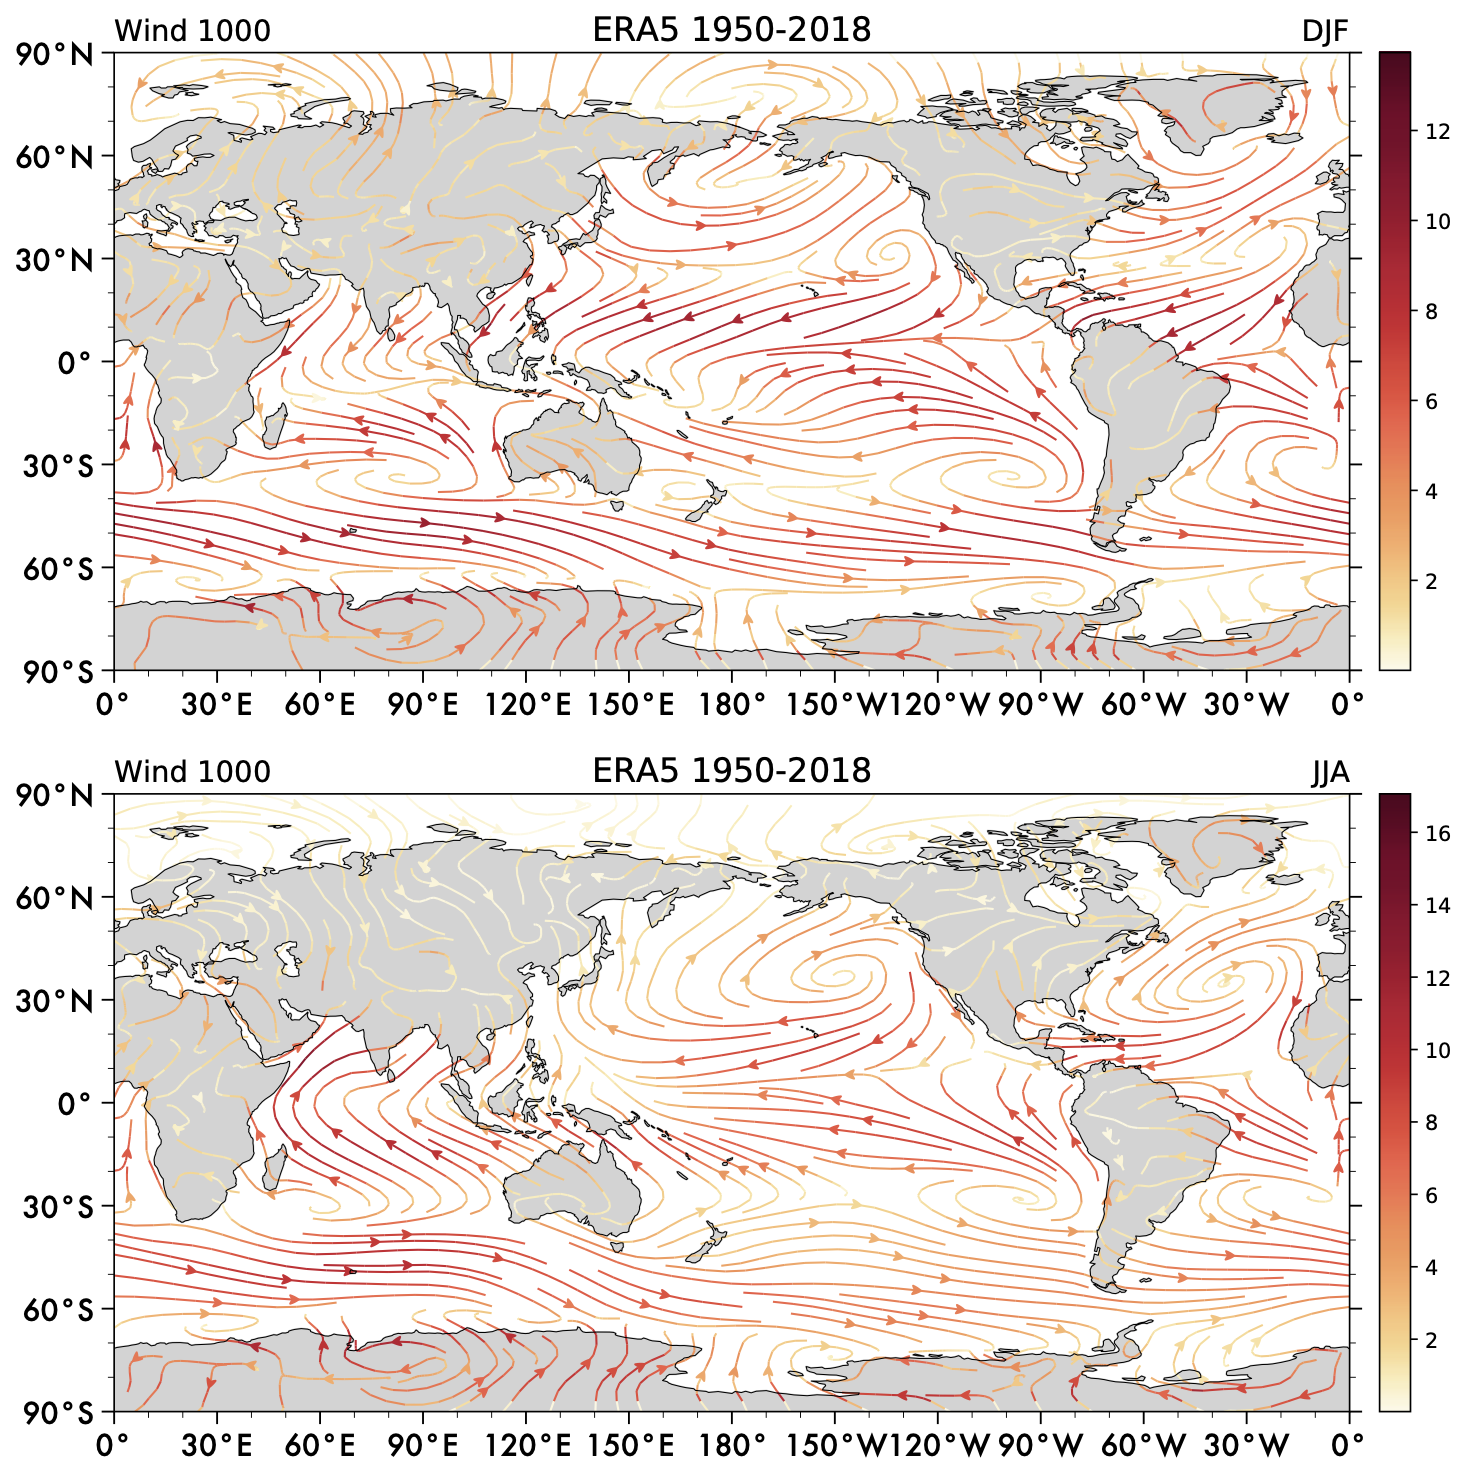
\includegraphics[width = .7 \textwidth]{figs/GD/Wind1000.png}
\caption{} \label{fig:}
\end{figure}

\subsection{The thermal structure of the
Ocean}\label{the-thermal-structure-of-the-ocean}

The temperature structure of the oceans is shown in Fig.
\texttt{fig:610}. The top panel shows the temperature near the surface
at a nominal depth of 5m. We notice that there is a strong latitudinal
gradient as the equatorial zone tends to have warmer temperatures and
colder areas develop towards the polar areas. It is simple to connect
this structure with the radiation balance indicating a positive balance
in the equatorial zone and a negative one in the polar regions.

However, the latitudinal structure is broken in several areas. There are
significant gradients along the Equator both in the Pacific and in the
Atlantic basins and in general the East side of the basin tend to be
colder than the West side. Furthermore significant cold area exist along
the Equator in the Pacific in the East and along the South American
coast. A careful analysis shows that also in the midlatitudes there are
strong East-West differences, as the East side of the basins tend to be
warmer than the West. And just to avoid confusion we have to become
familiar with the fact that the East side of an ocean basin is bordering
with the \emph{West coasts} of the respective continent.

\begin{figure}
\centering
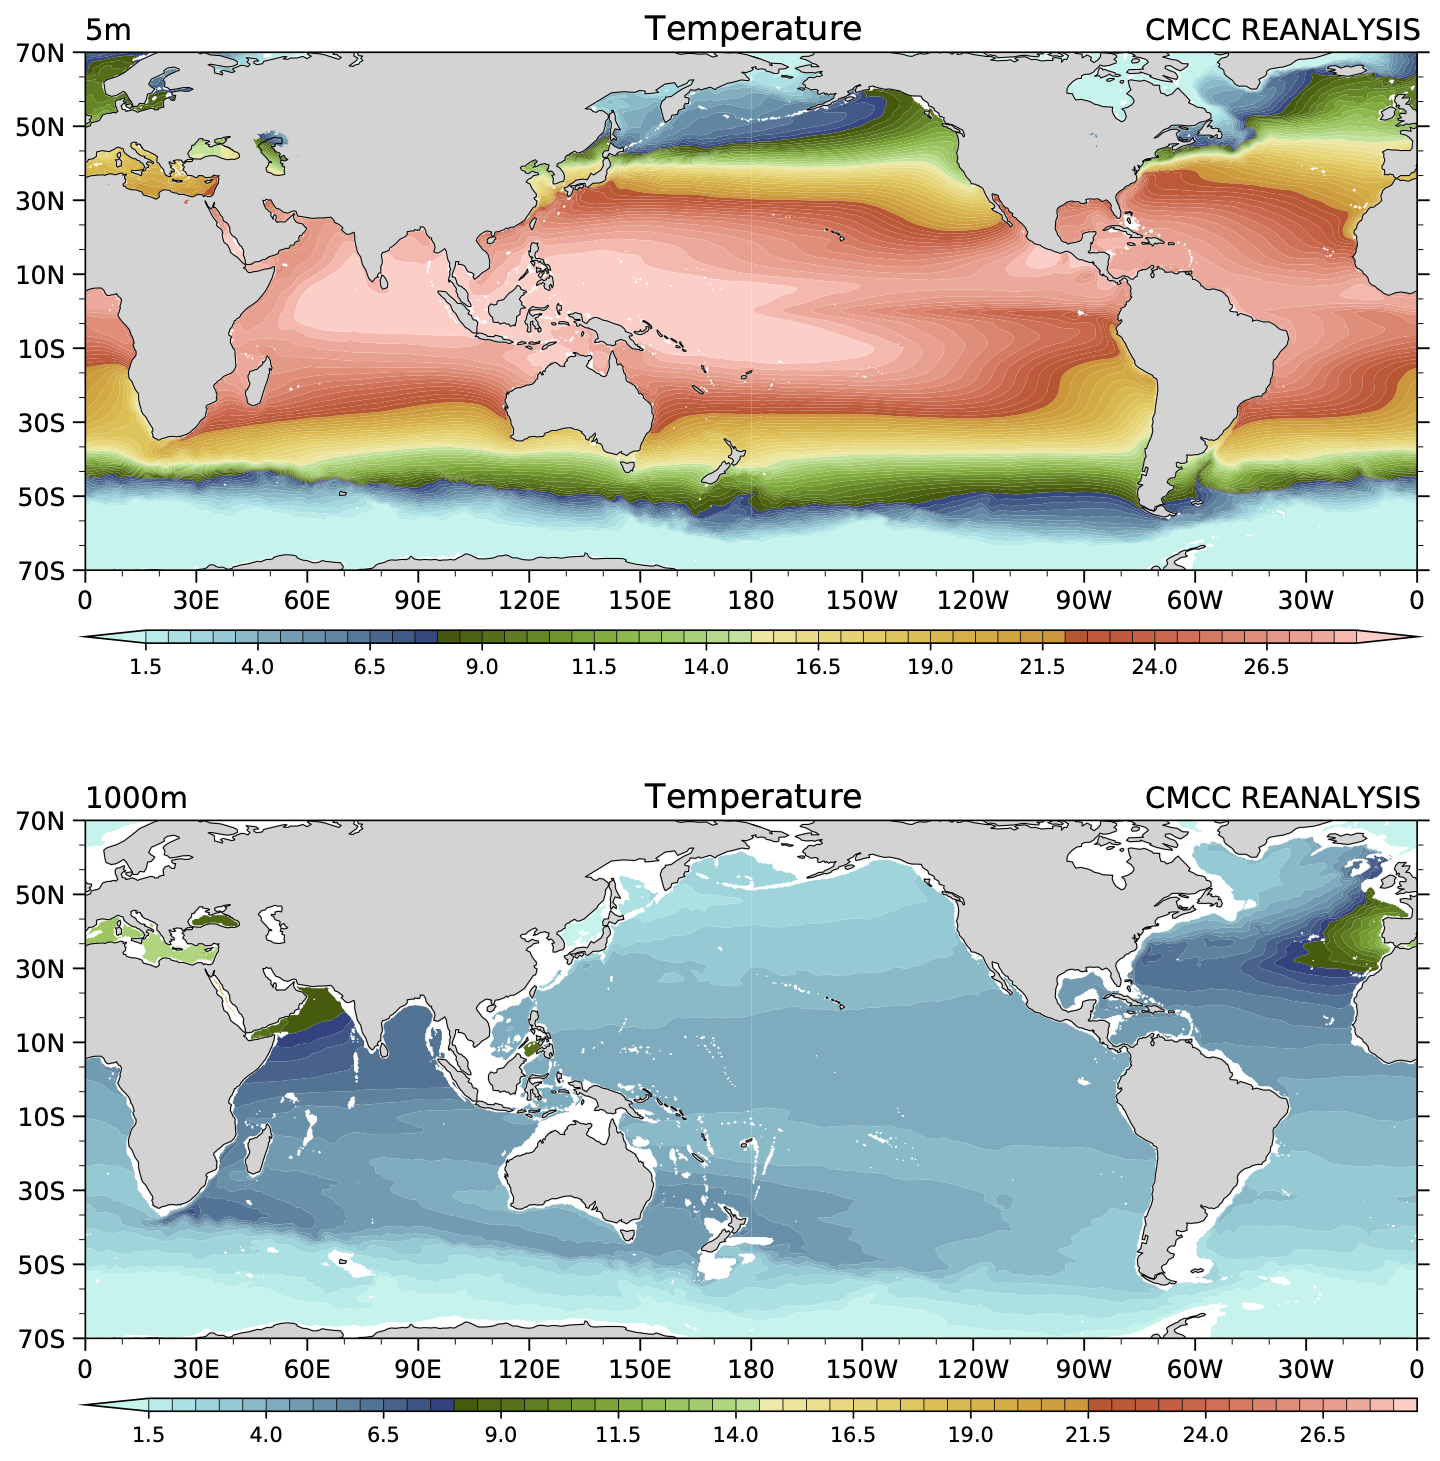
\includegraphics[width = .7 \textwidth]{figs/GD/Temp5-1000.png}
\caption{} \label{fig:}
\end{figure}

At the deeper depth pf 1000m (bottom panel) the ocean tends to be much
colder. We are using here the same scale to give a feeling of the
temperature drop. We can see that the general signature of the structure
that we have identified at the surface is still present, but there are
some interesting deviations.

In the North Atlantic the water is significantly warmer than the same
latitudes in the Pacific and it is easy to see that the origin of the
water is the Mediterranean that is contributing very warm waters to the
Atlantic via the Gibraltar Straits. The Mediterranean water penetrate
deeply into the Atlantic, basically up to the American coast.

\begin{figure}
\centering
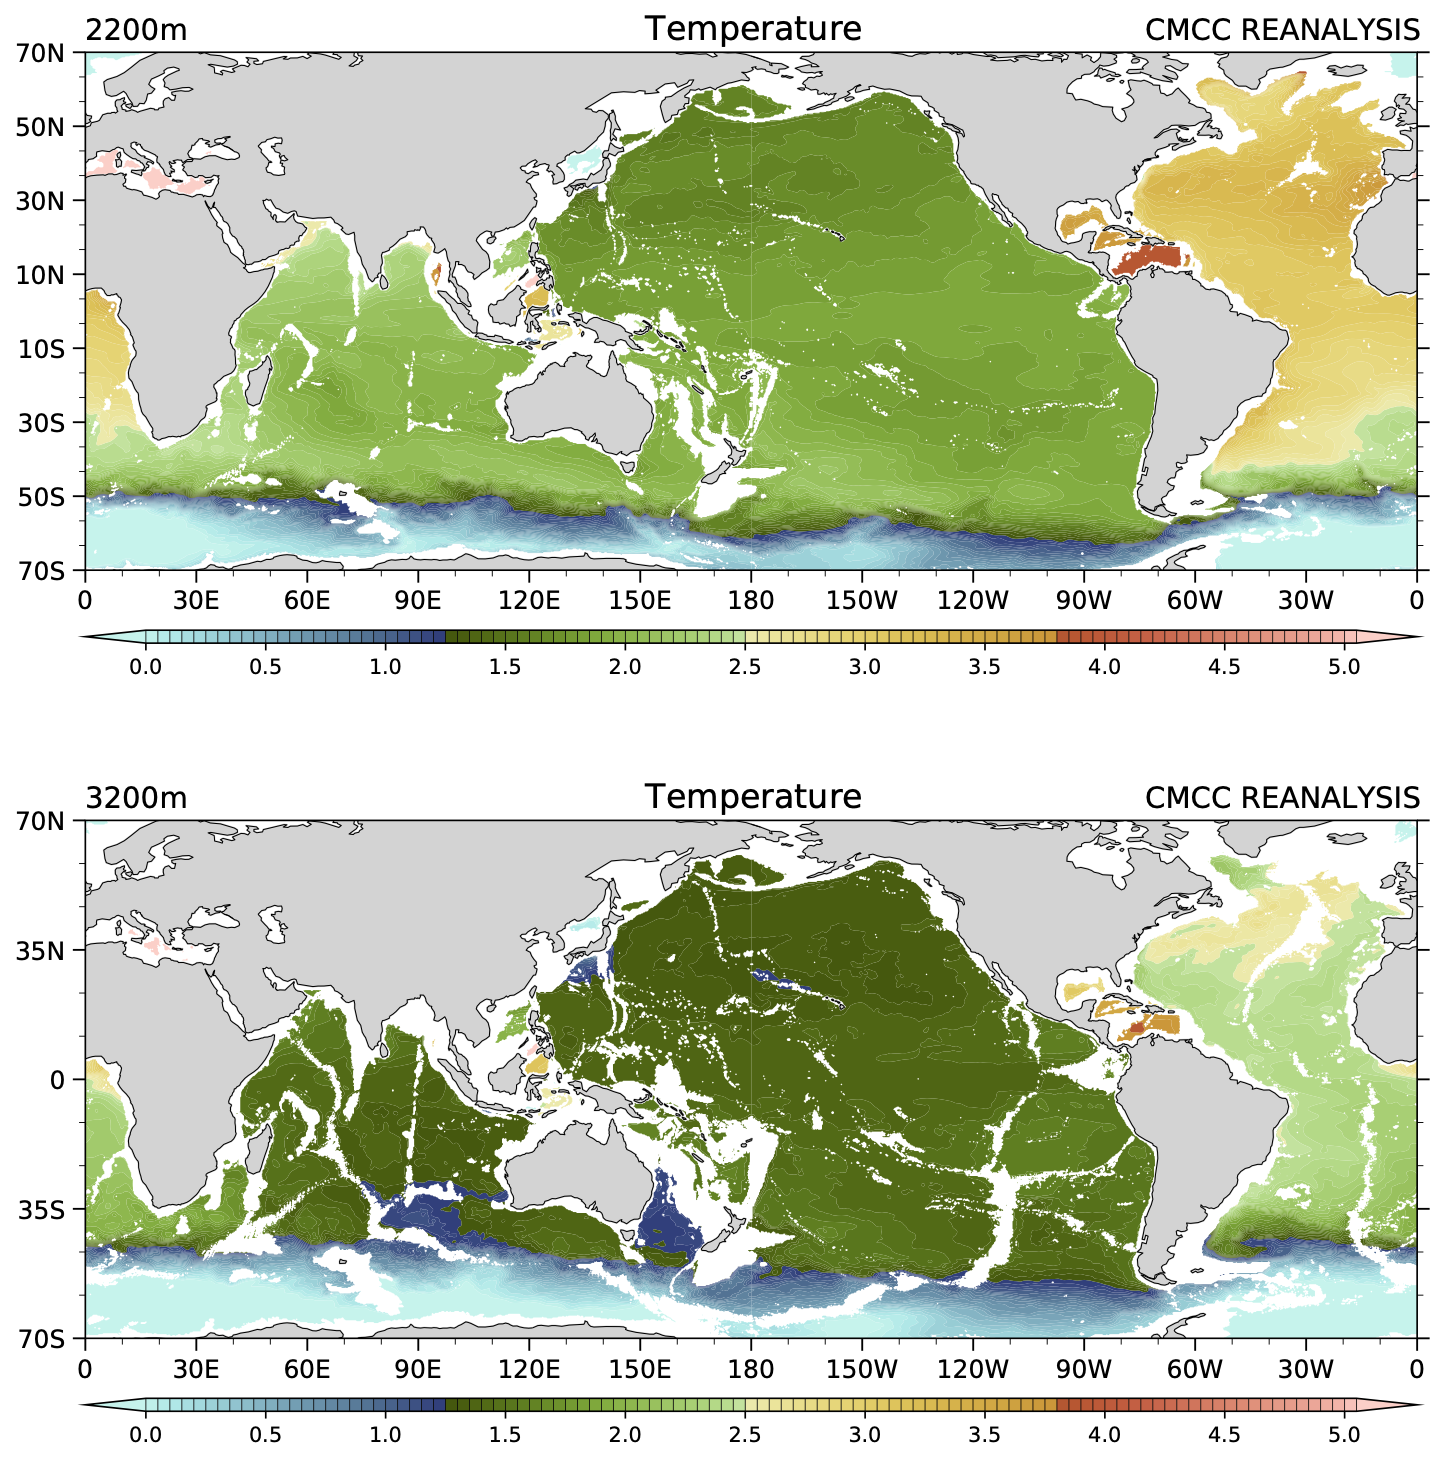
\includegraphics[width = .7 \textwidth]{figs/GD/Temp2200-3200.png}
\caption{} \label{fig:}
\end{figure}

Going even deeper (Fig. \texttt{fig:611}) we have to change drastically
the temperature scale. The typical temperature is now only a few
degrees. The Southern Ocean is very cold and the water is hovering
around 1.0 degree. The abyssal waters (Fig. \texttt{fig:612}) are
definitely colder and it is only the pressure that keeps them from
freezing when they get close to zero degrees. We cam also see
empirically how the average depth of the oceans is close to 4000 meter
as there are only limited areas that reach deeper depths. A precise,
quantitative calculation will yield the value of 4200? meters for the
average depth of the oceans.

\begin{figure}
\centering
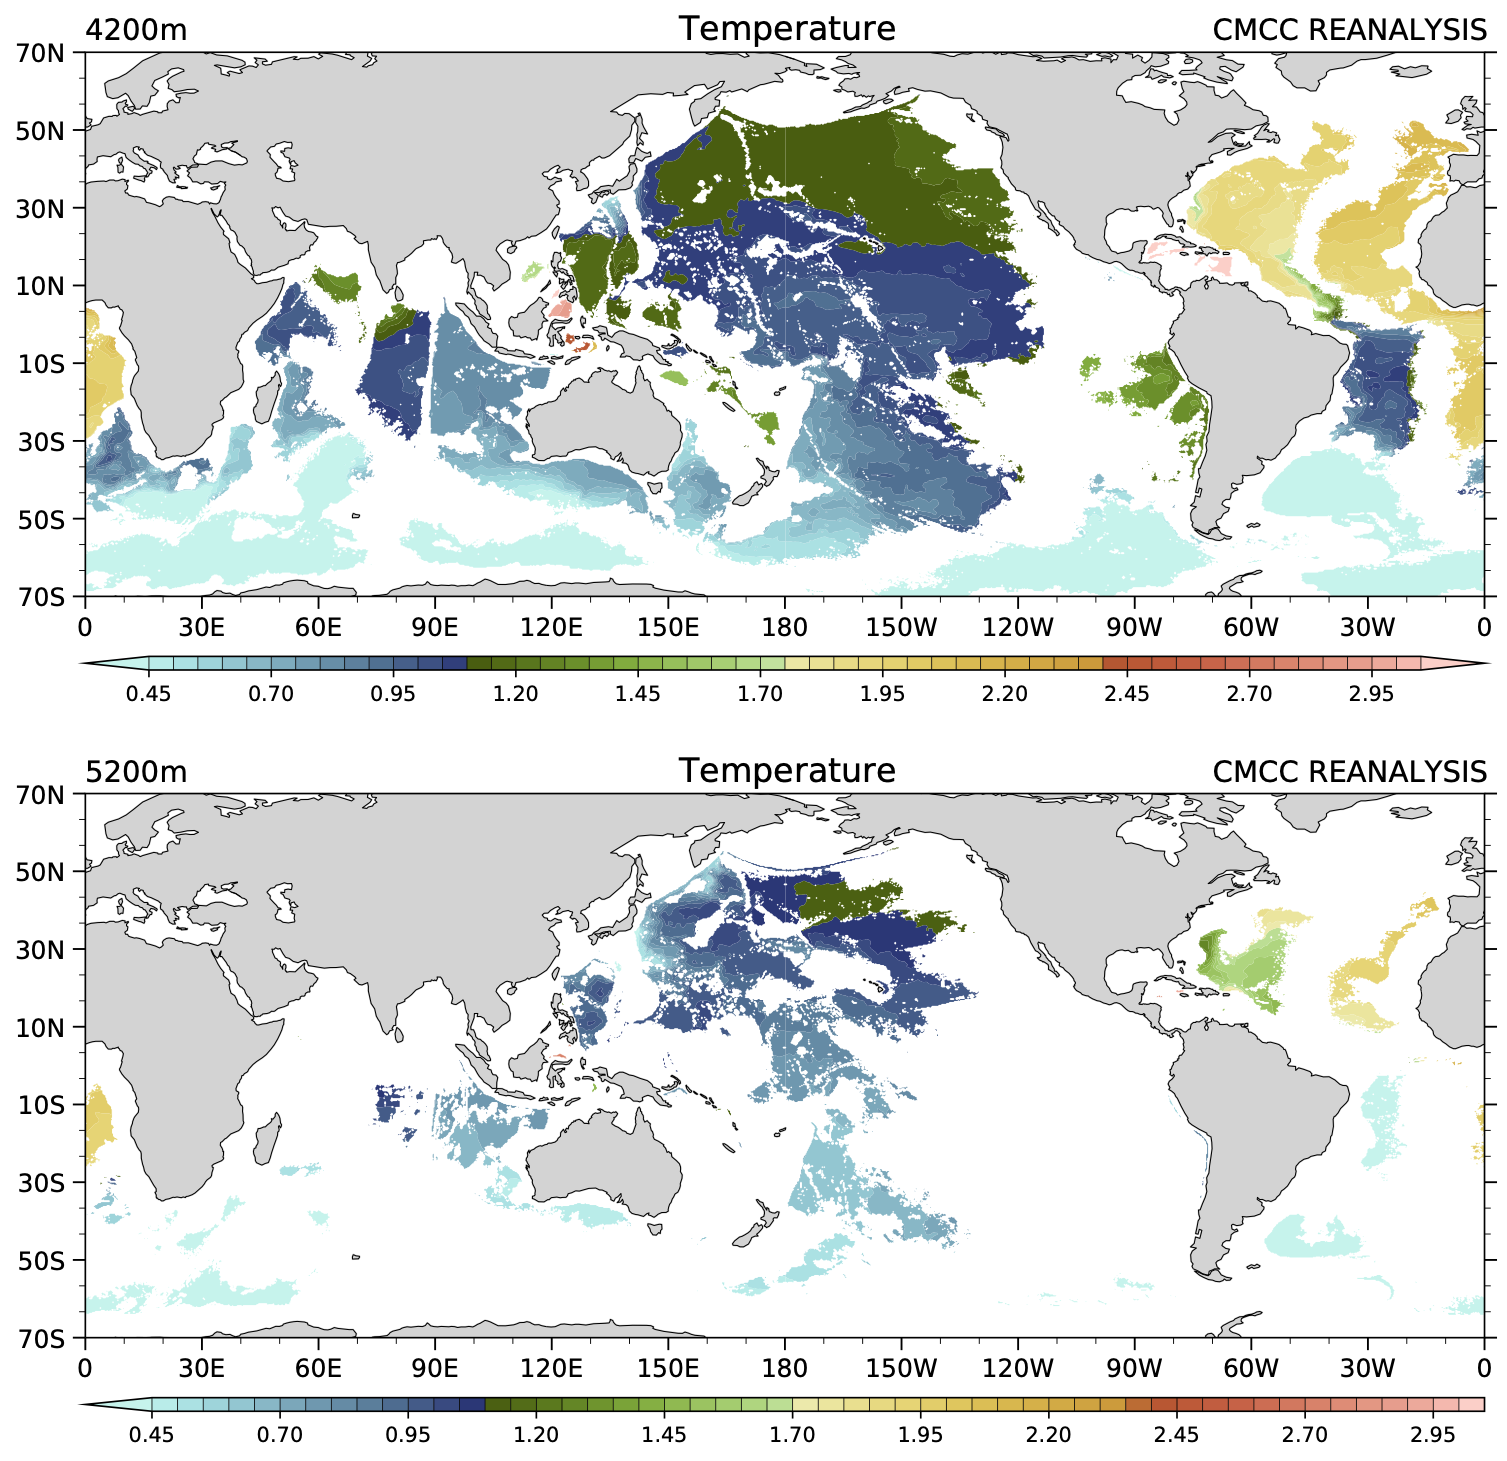
\includegraphics[width = .7 \textwidth]{figs/GD/Temp4200-5200.png}
\caption{} \label{fig:}
\end{figure}

A qualitative look at this pictures already gives the impression of the
diversity among the various Oceans. We can guess that the dynamics of
the Souther Ocean, colder and basically unimpeded by continental
boundaries in a single circle around the South Pole is probably going to
be different from all others. By the same token, the warmer Atlantic,
deeply affected by the Mediterranean inflow is going to show different
characteristics from the Northern Pacific, colder and larger.

A closer look will reveal further differences between the mid-latitude
oceans and the tropical oceans. Looking at the North Atlantic (Fig.
\texttt{fig:613}) we notice the strong gradients along the North
American Coast that persists up to 1000m. Strong temperature gradients
are presumably to be connected to the existence of currents, but we will
need to check the density, depending on the salinity later, to be really
sure. Anyway, this picture is giving a strong indication of the
existence of something remarkable and intense along the western boundary
of the Atlantic ocean.

\begin{figure}
\centering
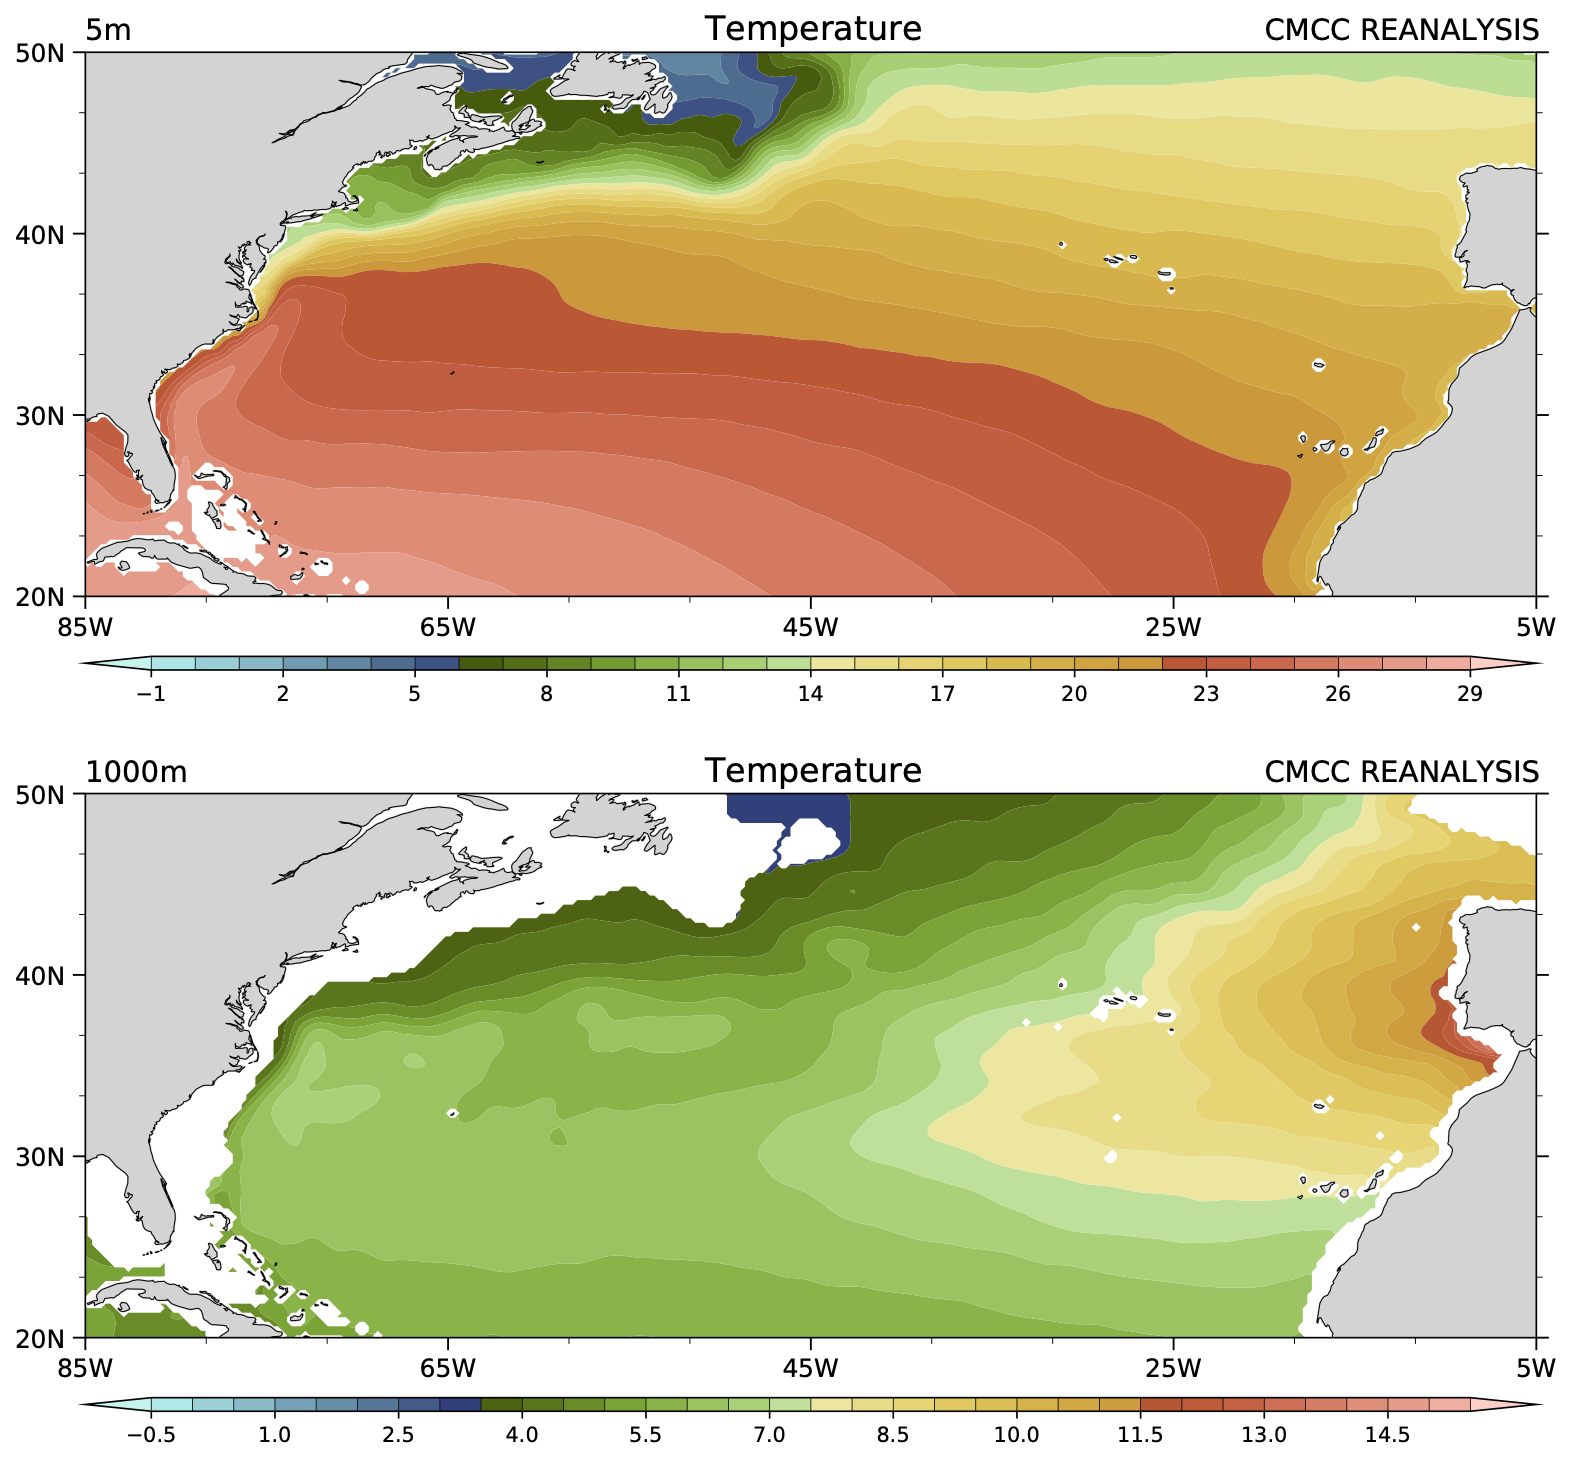
\includegraphics[width = .7 \textwidth]{figs/GD/Gulf1000.png}
\caption{} \label{fig:}
\end{figure}

Warm waters are protruding from the Gibraltar Straits into the Atlantic.
They are not very visible at the surface, but they are remarkably well
clear at depth, for instance the 100m shown here. The warm water is
sinking, indicating that its density is higher than the surrounding
water, notwithstanding the higher temperature.

The North Pacific shows something similar along the Japan coast and
therefore we can start to suspect that this has to do with the presence
of the continental boundary. Without the Mediterranean, the vertical
structure is more uniform and we can notice a progressive cooling of the
water.

\begin{figure}
\centering
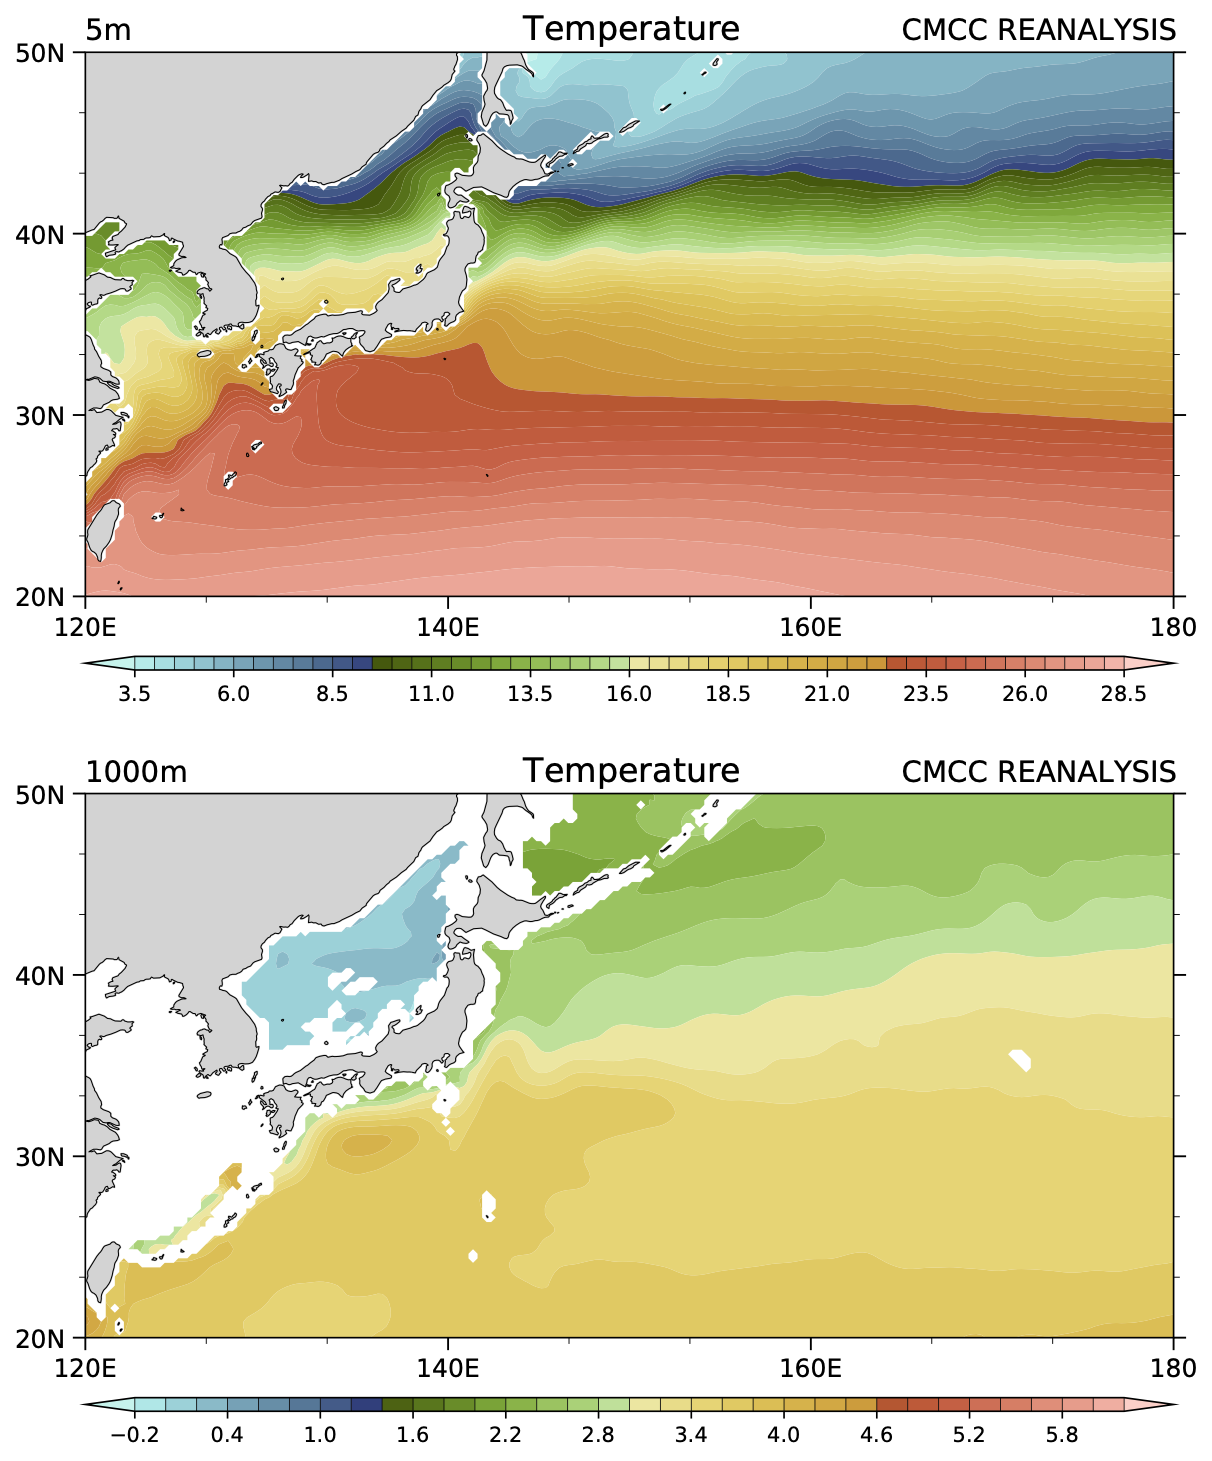
\includegraphics[width = .7 \textwidth]{figs/GD/Kur1000.png}
\caption{} \label{fig:}
\end{figure}

The preliminary analysis is giving us hints of a strong vertical
structure of the oceans, soit may be useful to look at the vertical
distribution somewhat more in detail. Fig. \texttt{fig:6100} shows a
North-South section along the longitude of 25W, roughly in the middle of
the Atlantic Ocean. The bottom panel reaches to 5000m, it is very
evident the strong stratification of the ocean. An area of high
variation, where the temperature cools down quickly, appears around
800-1000m, more prominent in the Southern Hemisphere, below that the
ocean is more uniform and very cold. This sharp transition region is
called \emph{thermocline}.

It is interesting to note how layers of water of the same temperature
can reach the surface, as it can be seen from the picture and, in more
detail, from the top panel. The layers connect even considerable depths,
like is the case for the very cold water around 2-4 C that rises from
the bottom of the Southern Ocean surfacing into the Antarctic region.

\begin{figure}
\centering
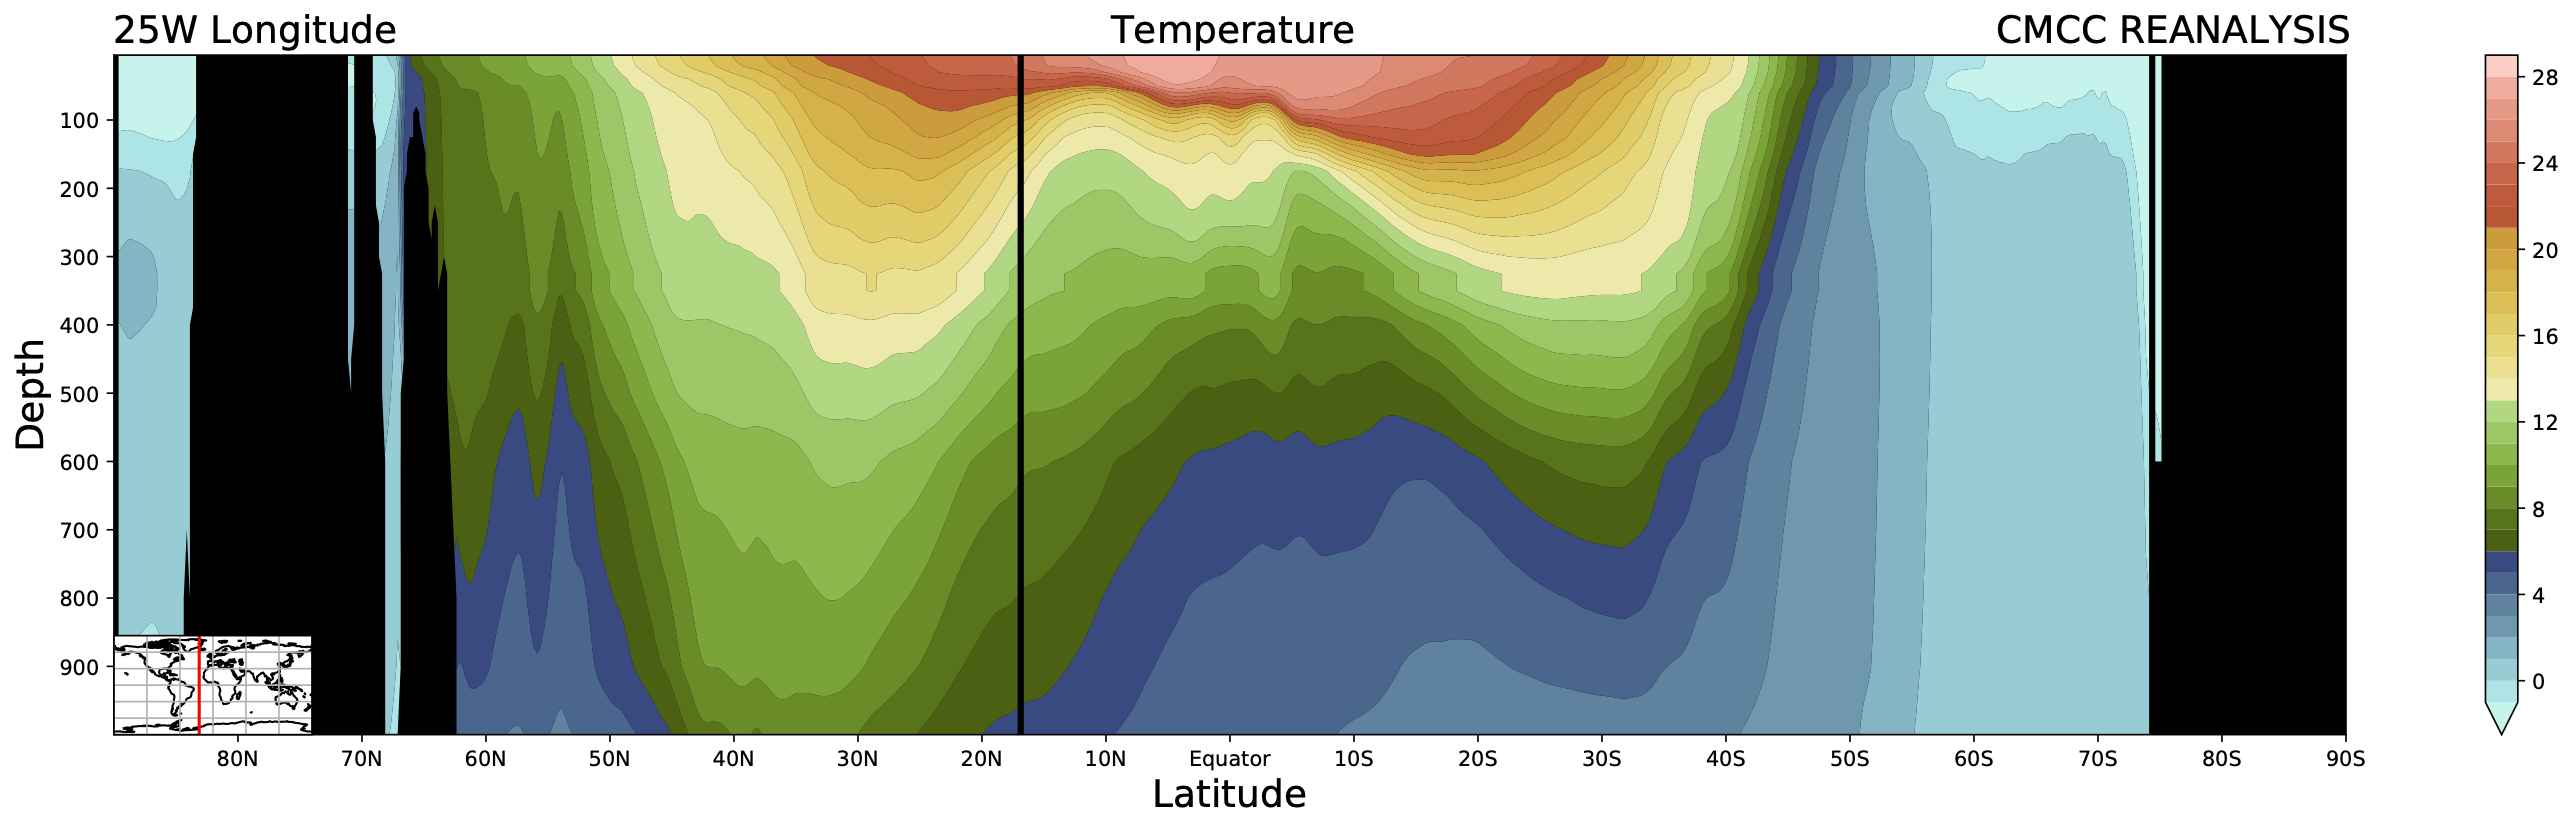
\includegraphics[width = .7 \textwidth]{figs/GD/Sect25W1000.png}
\caption{} \label{fig:}
\end{figure}

\begin{figure}
\centering
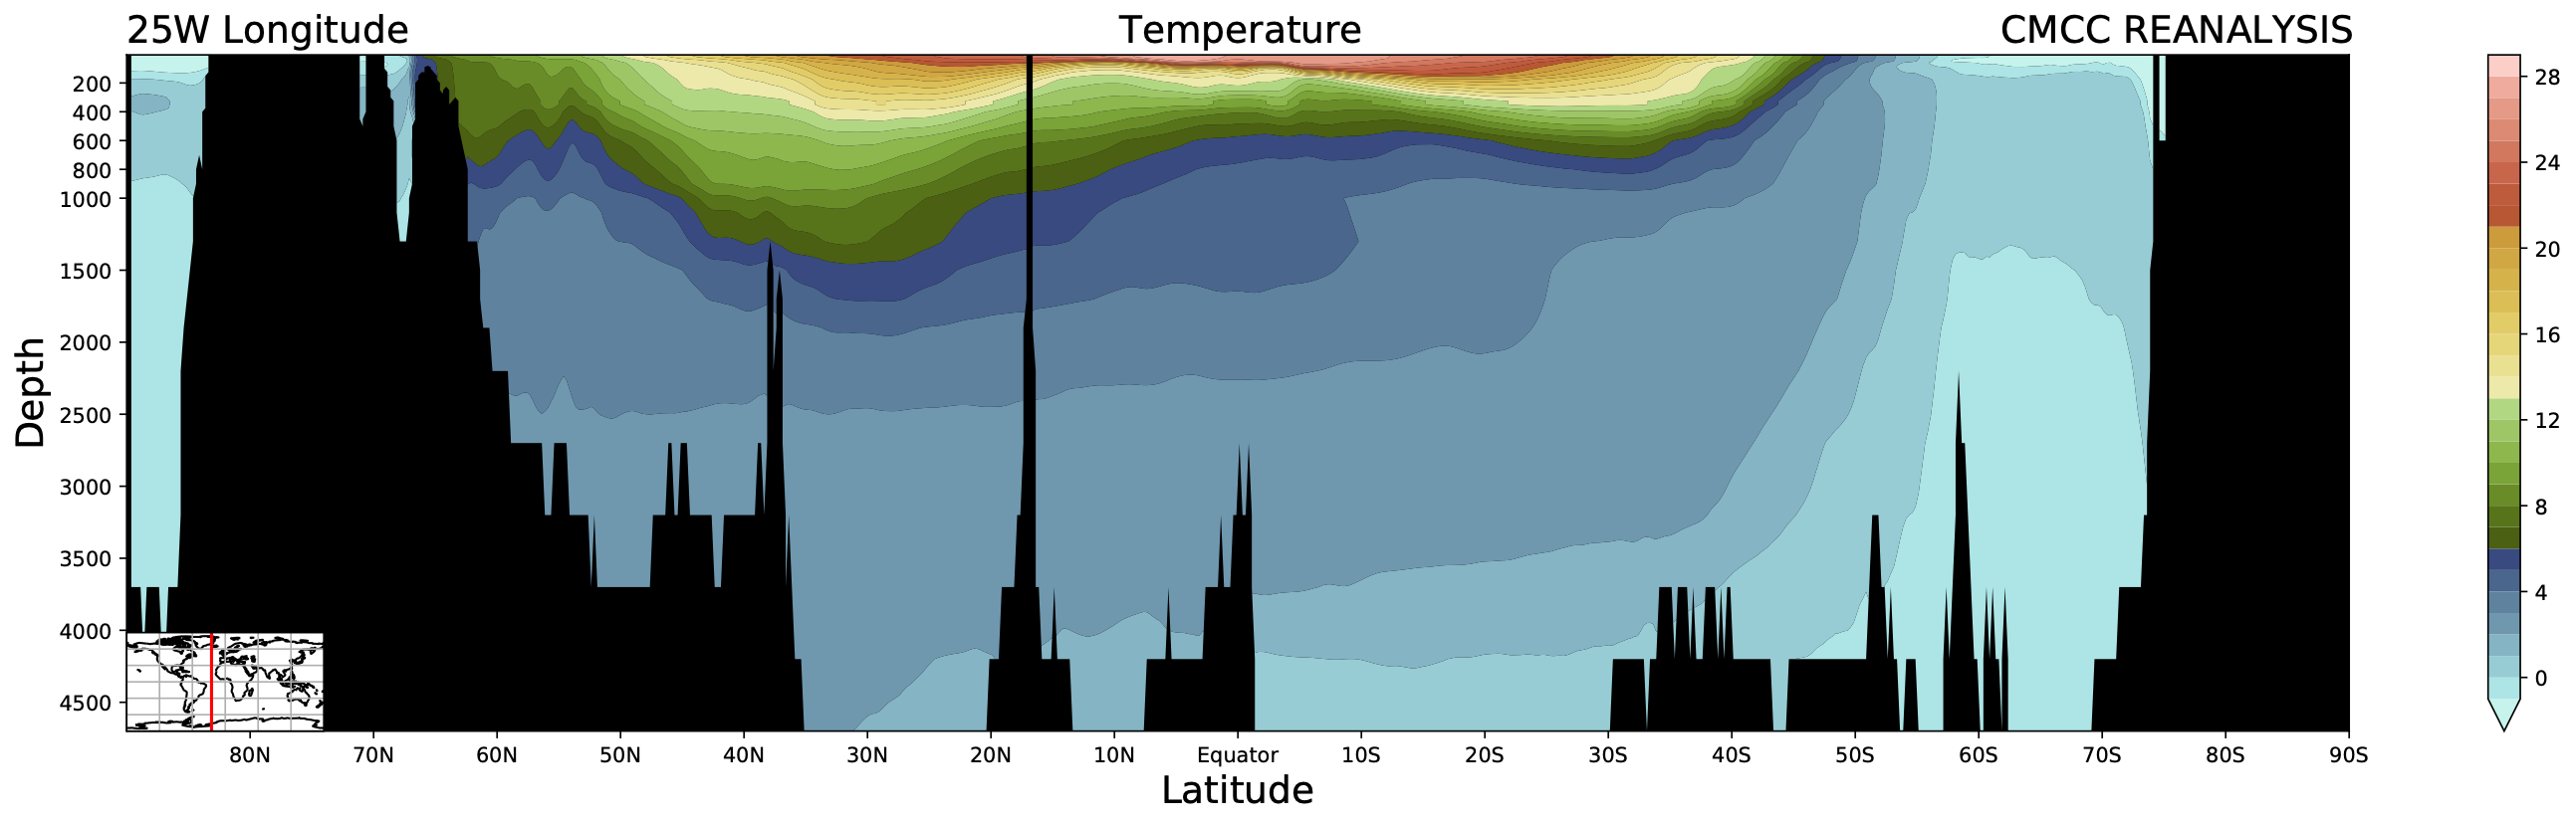
\includegraphics[width = .7 \textwidth]{figs/GD/Sect25W5000.png}
\caption{} \label{fig:}
\end{figure}

The signature of the Mediterranean outflow can be seen in the asymmetry
between the hemispheres that pushes relatively warmer water down in the
Northern Atlantic relatively to the Southern part of the ocean.

\begin{figure}
\centering
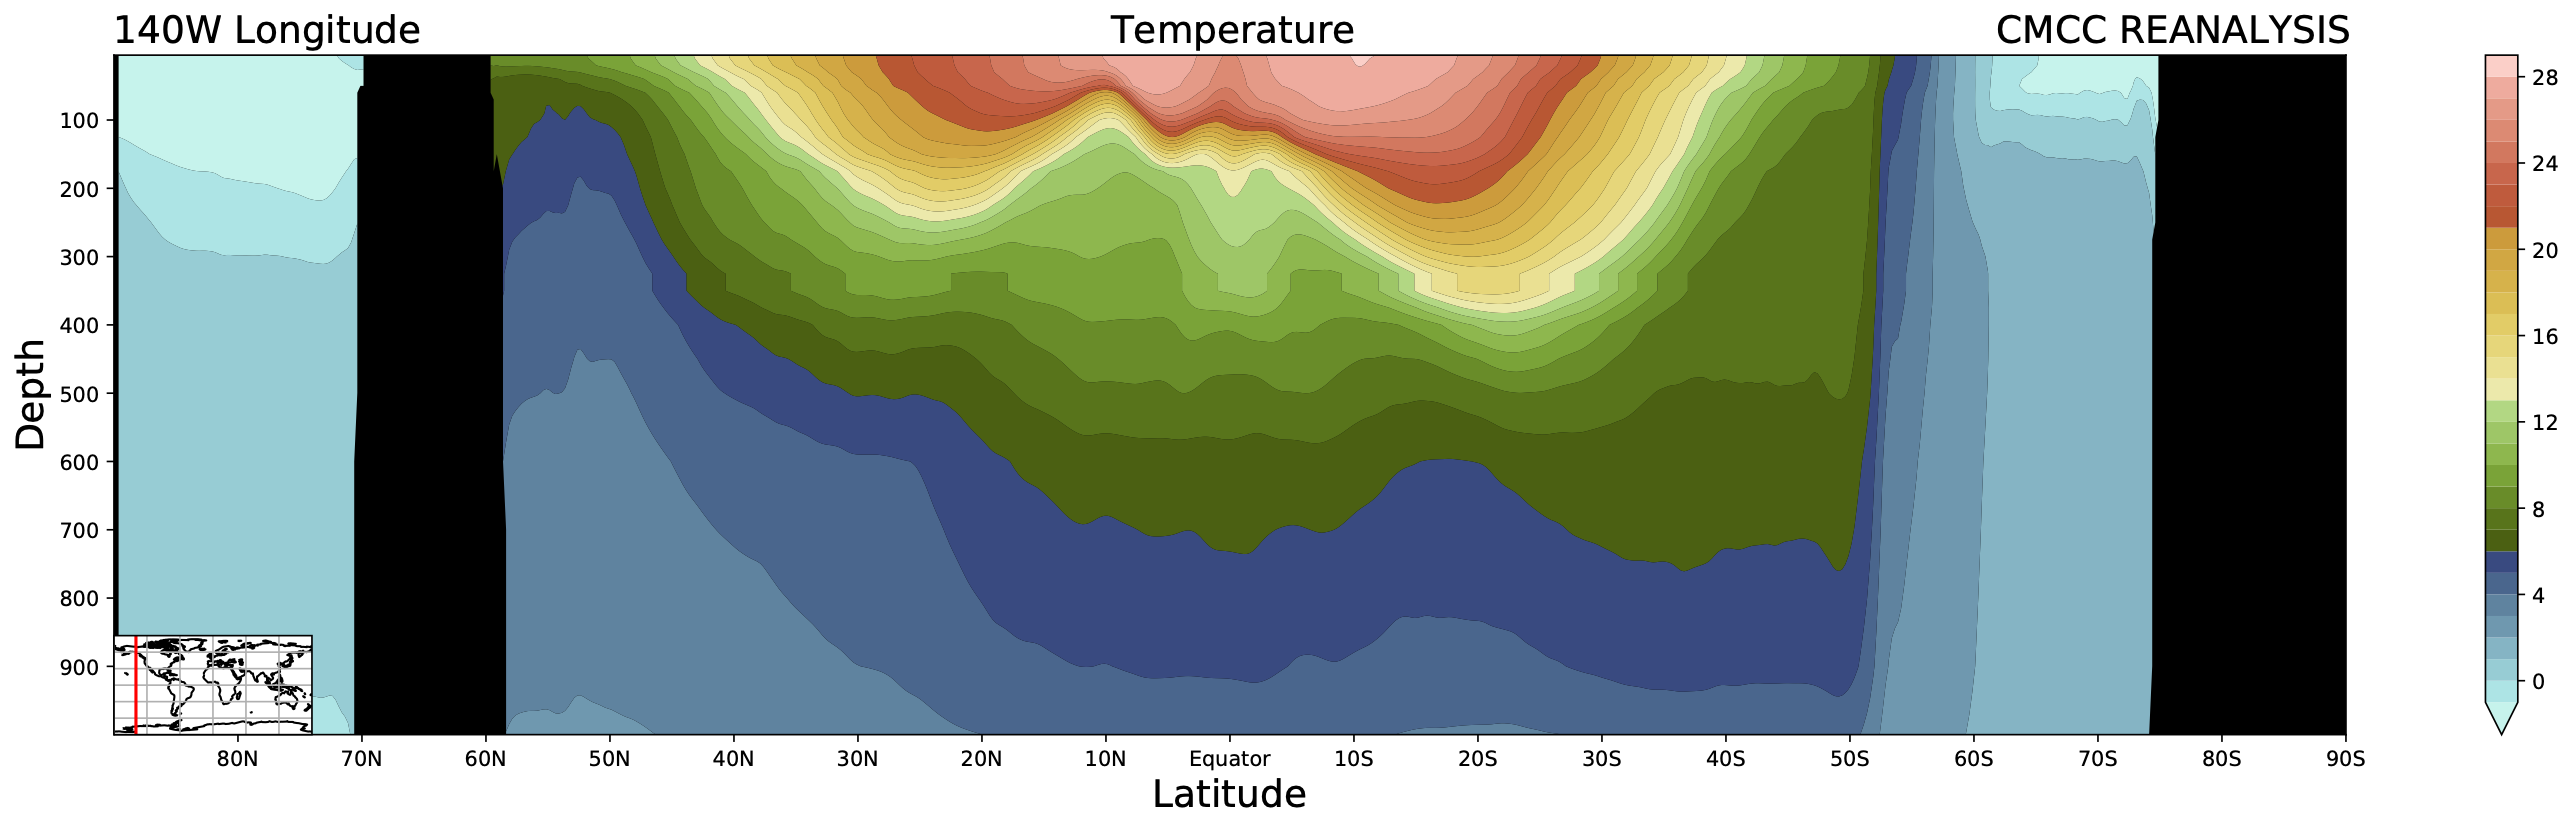
\includegraphics[width = .7 \textwidth]{figs/GD/Sect140W1000.png}
\caption{As in Fig. \texttt{fig:6100} but for 140W longitude}
\end{figure}

\begin{figure}
\centering
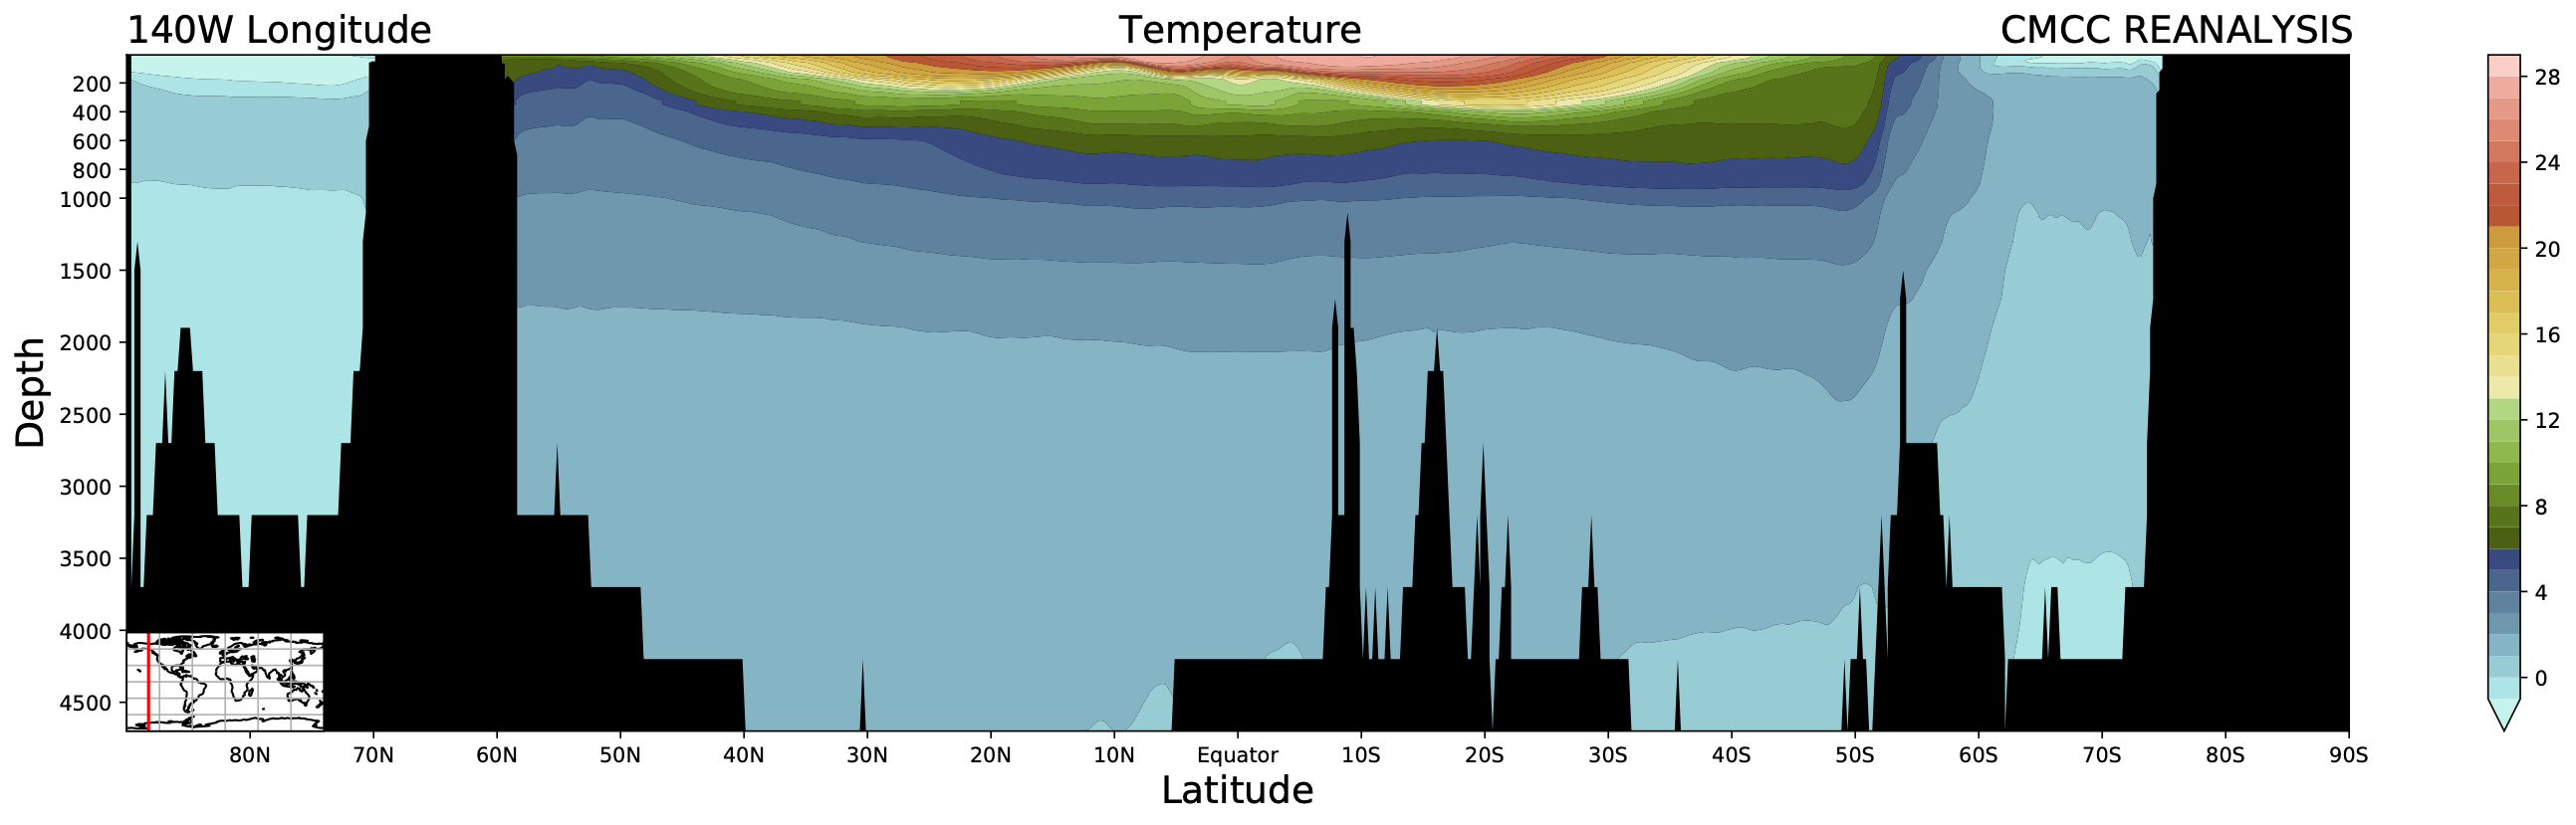
\includegraphics[width = .7 \textwidth]{figs/GD/Sect140W5000.png}
\caption{As in Fig. \texttt{fig:6100a} but for 140W longitude}
\end{figure}

Looking at a similar section in the middle of the Pacific Ocean at 140W
longitude we see a different situation. The relatively warm waters are
confined to a much shallower region confined to the subtropics. In this
basin is also more noticeable a phenomenon that was present also in the
Atlantic, namely the raising of cold water in the equatorial region that
is the signature of the cold tongue of equatorial water that lays in the
equatorial Pacific Ocean. Also in this case the layers of different
temperature reach the surface at different latitudes. Especially in the
Southern Hemisphere is possible to see the deep, cold abyssal water
connecting with the surface at very high southern latitudes.

\begin{figure}
\centering
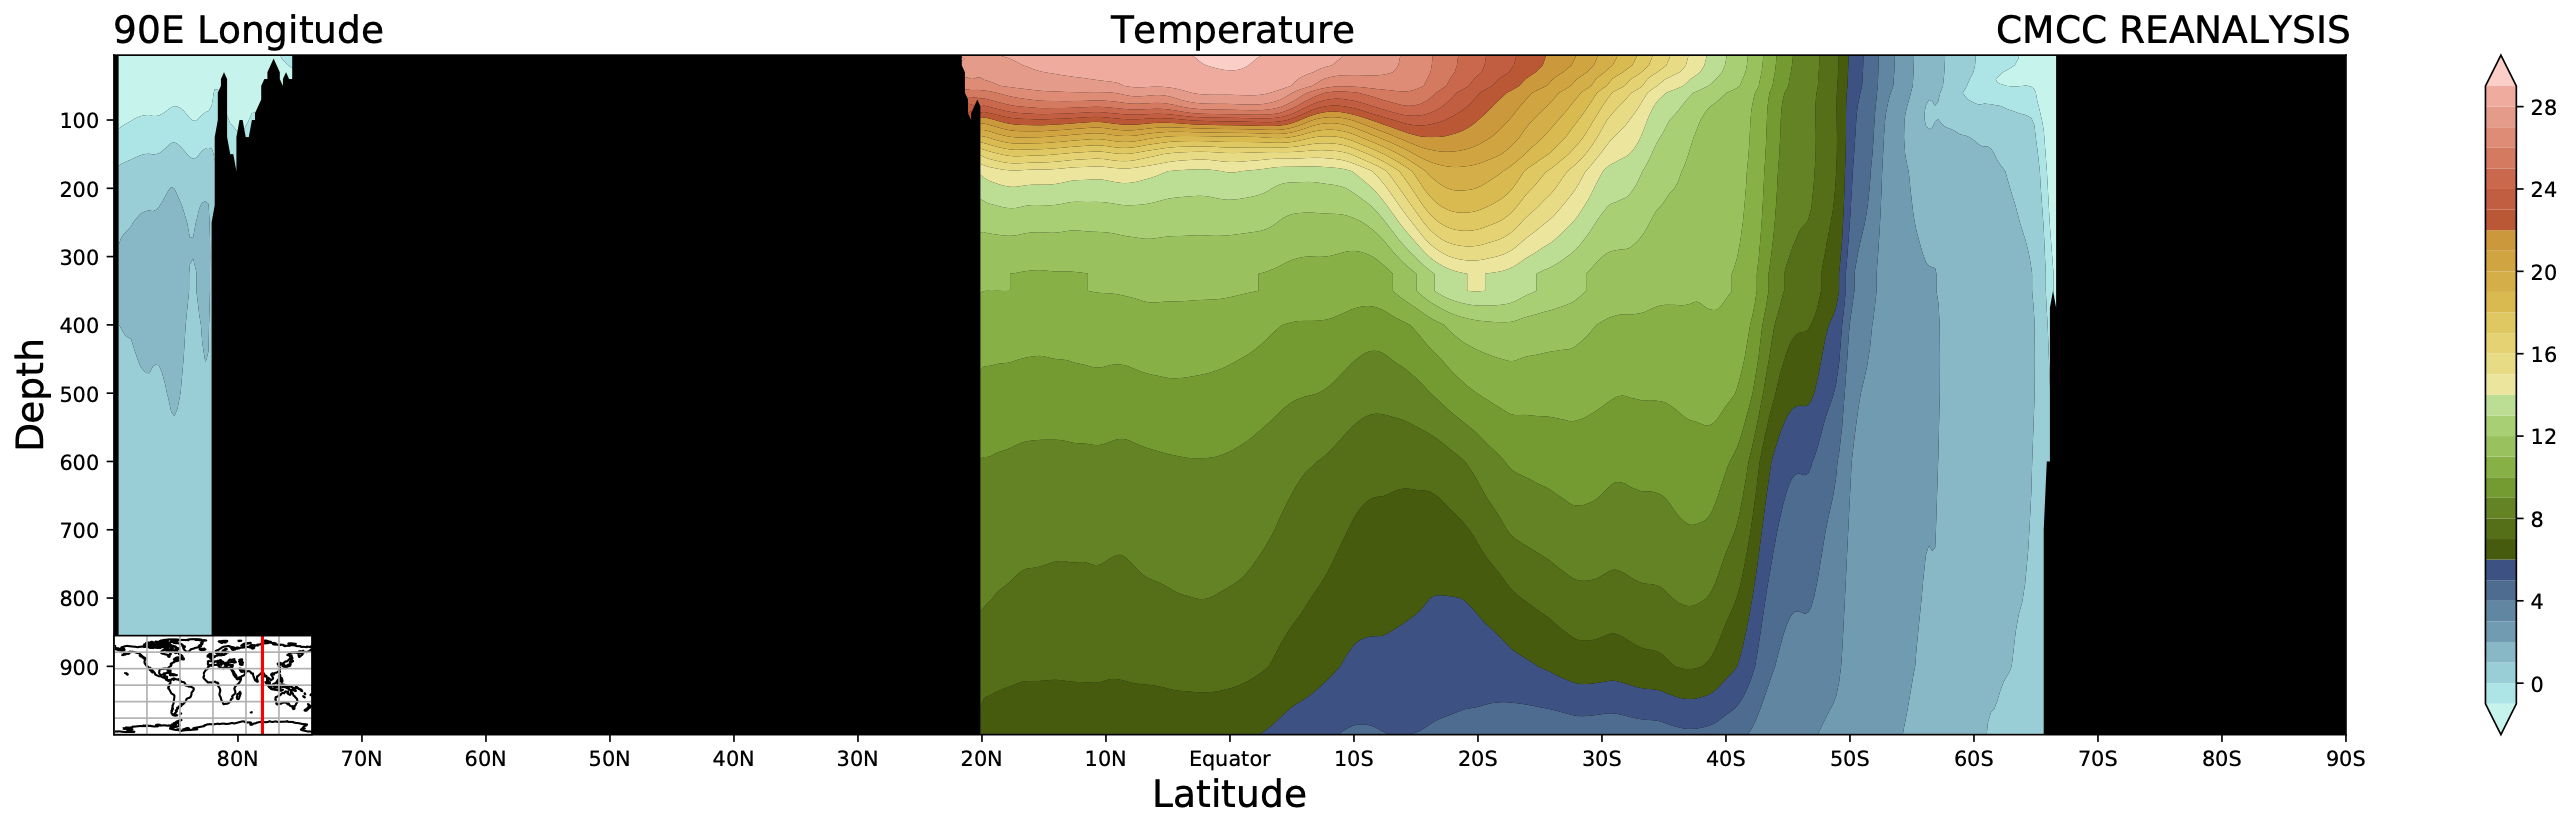
\includegraphics[width = .7 \textwidth]{figs/GD/Sect90E1000.png}
\caption{As in Fig. \texttt{fig:6100} but for 90E longitude}
\end{figure}

\begin{figure}
\centering
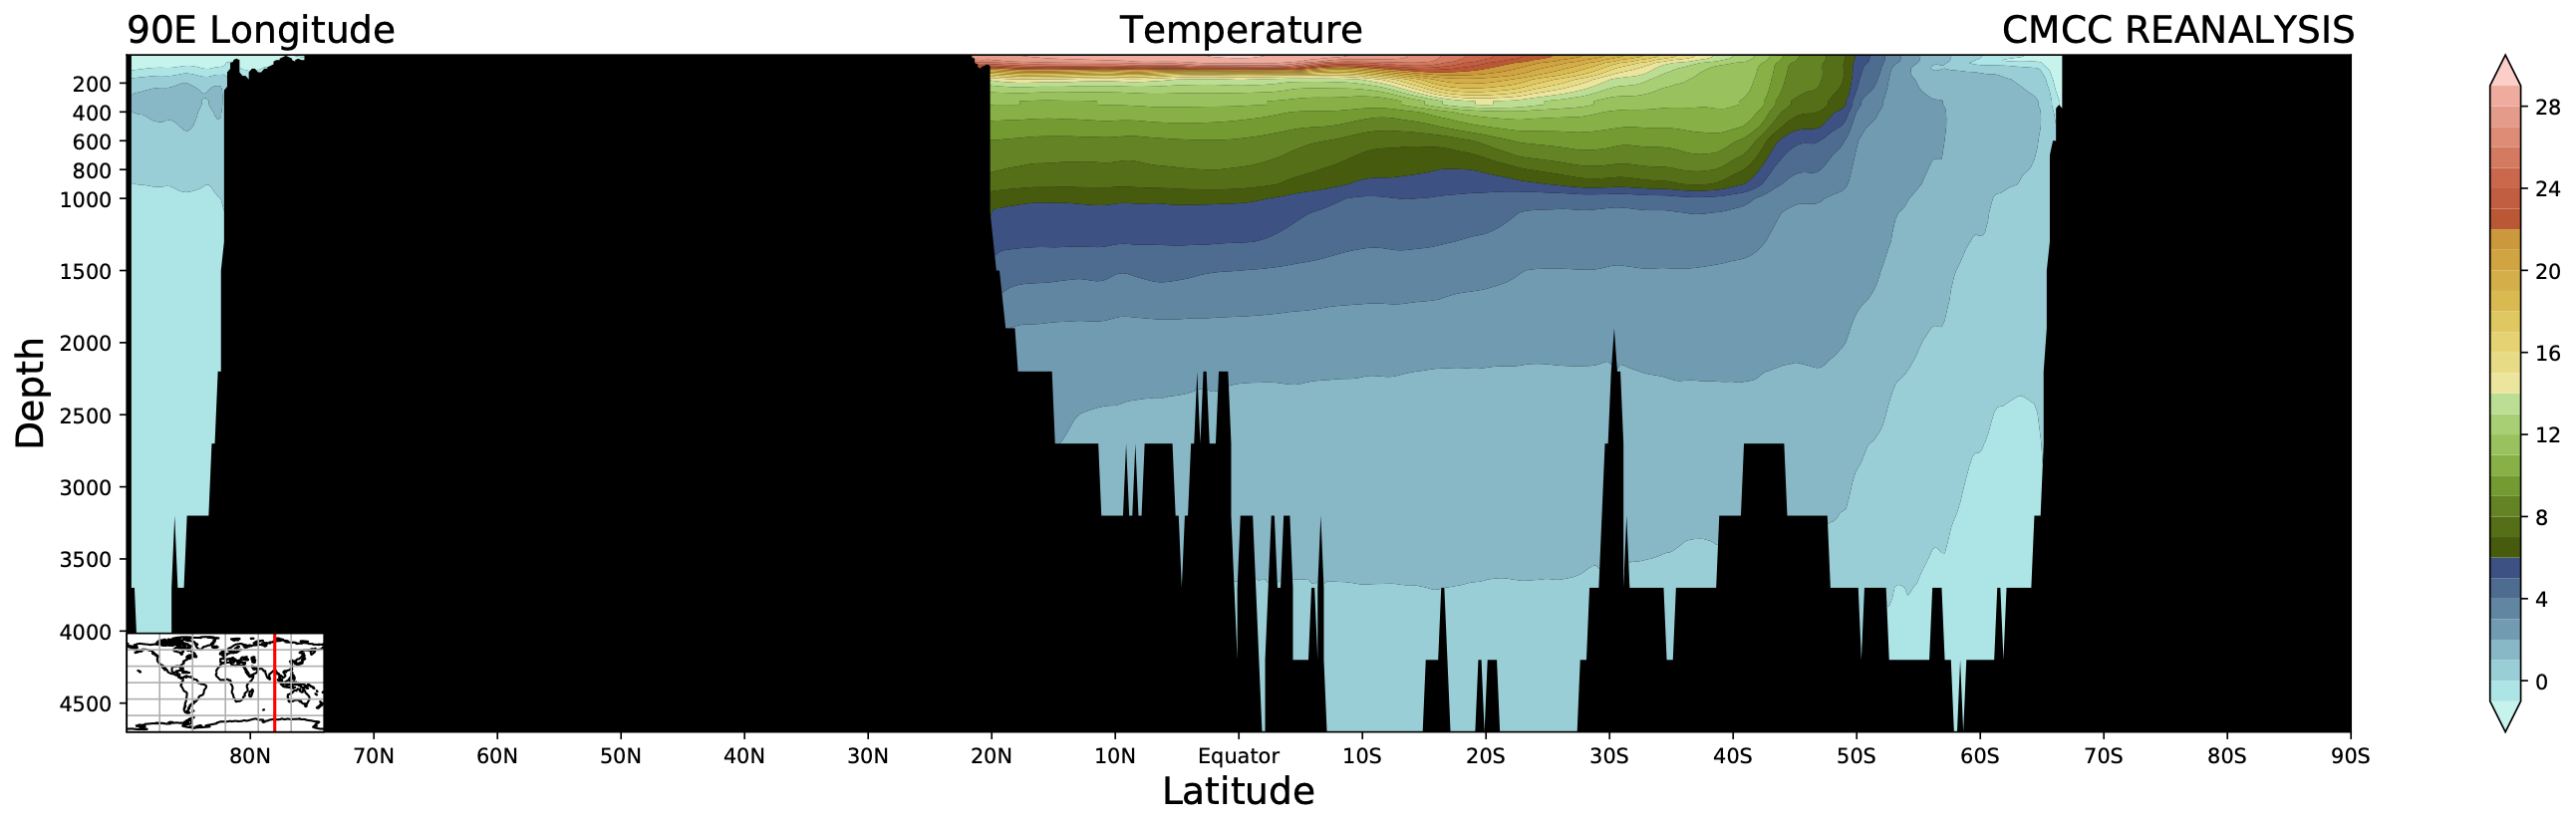
\includegraphics[width = .7 \textwidth]{figs/GD/Sect90E5000.png}
\caption{As in Fig. \texttt{fig:6100a} but for 90E longitude}
\end{figure}

The Indian Ocean (Fig. \texttt{fig:6102}) shown here as a section
cutting essentially through the Bay of Bengal, shows a similar strong
stratification, but there are only weak signs of an equatorial upwelling
of cold water.

\begin{figure}
\centering
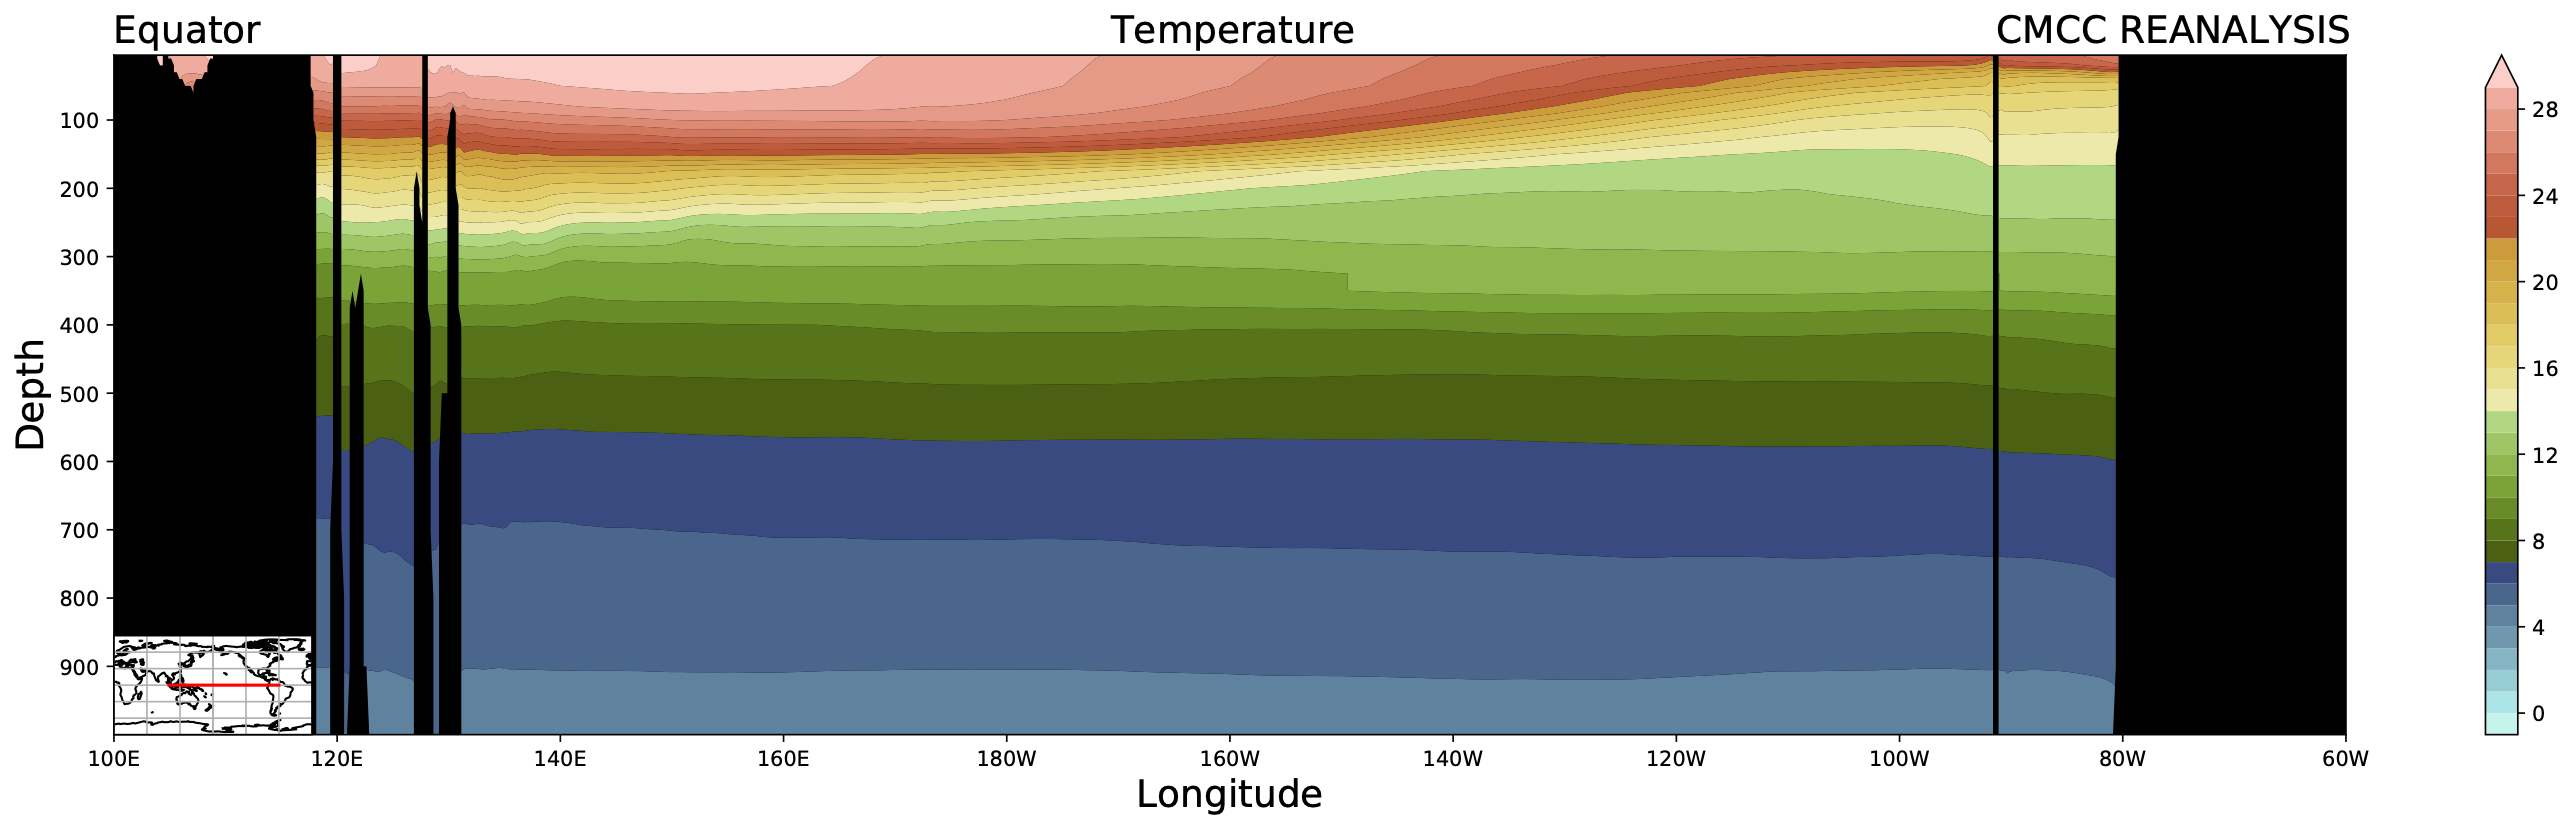
\includegraphics[width = .7 \textwidth]{figs/GD/SectEquator1000.png}
\caption{} \label{fig:}
\end{figure}

We can gain more insights in the equatorial structure by looking at a
longitudinal section along the Equator in the Pacific (Fig.
\texttt{fig:6103}). The thermocline is clearly visible, but there is a
clear east-west inclination of the thermocline with a significant
deepening in the West Pacific and a mush shallower layer in the East,
close to the South American coast. The thermal gradient is really strong
and it crosses several degrees in a few tens of meters.

\subsection{The salinity structure of the
Ocean}\label{the-salinity-structure-of-the-ocean}

The salinity structure of the oceans is shown in Fig. \texttt{fig:710}.
The top panel shows the salinity near the surface at a nominal depth of
5m. We notice that there is a complex structure with low salinity
(fresher) waters at the poles and progressively more saline water moving
towards the Equator, but then salinity decreases again at the equator.
It is probably instructive to look at the latitudinal distribution of
the precipitation (Fig. \texttt{fig:70a}). We can notice that the peaks
of precipitation in the midlatitude and at the Equator are correlated
with the low-salinity areas, whereas the subtropical regions are regions
of strong evaporation, whose signature is the high salinity of the
surface waters.

The Pacific Ocean is fresher than the Atlantic or even the Indian Ocean.
We can see from the map at 1000m that sources of saline waters are
marginal seas like the Mediterranean and the Persian Gulf. These areas
are evaporative basins that produce water so saline that it dominates
over the temperature effect and becomes denser so that we can find
Mediterranean water nelow the surface.

\begin{figure}
\centering
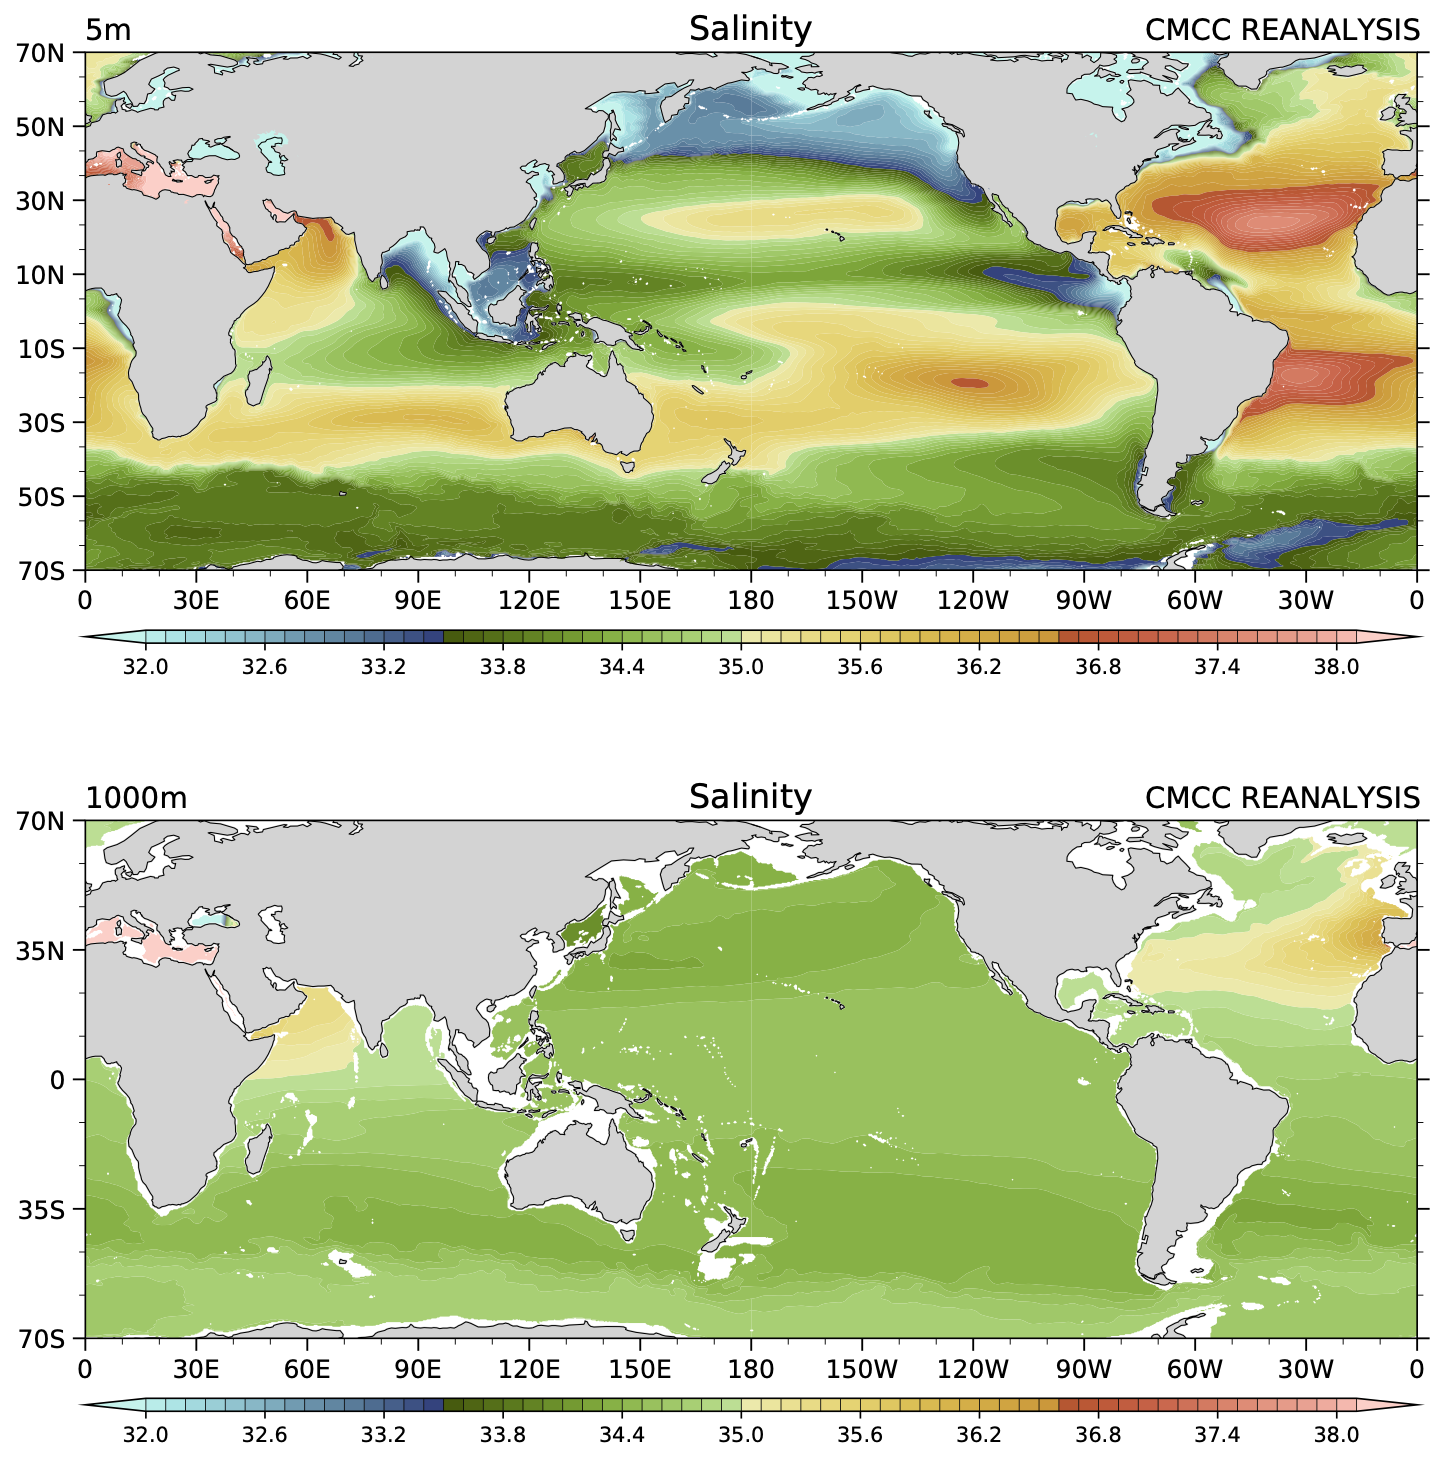
\includegraphics[width = .7 \textwidth]{figs/GD/Sal5-1000.png}
\caption{} \label{fig:}
\end{figure}

The effect of the precipitation is less visible at the deeper depth pf
1000m (bottom panel), where the ocean tends to be fresher and more
uniform. We are using here the same scale to give a feeling of the
changes in salinity, except for the Atlantic and the east Indian Ocean,
the salinity is around 34 psu. The situation does not change much lower
down (Fig. \texttt{fig:7110}).

The effect of the runoff from major river systems is visible along the
Atlantic coast of South America where the Amazon river discharges and in
the Bay of Bengal and around Indochina from the run-off the major rivers
there, the Ganges and the Mekong.

\begin{figure}
\centering
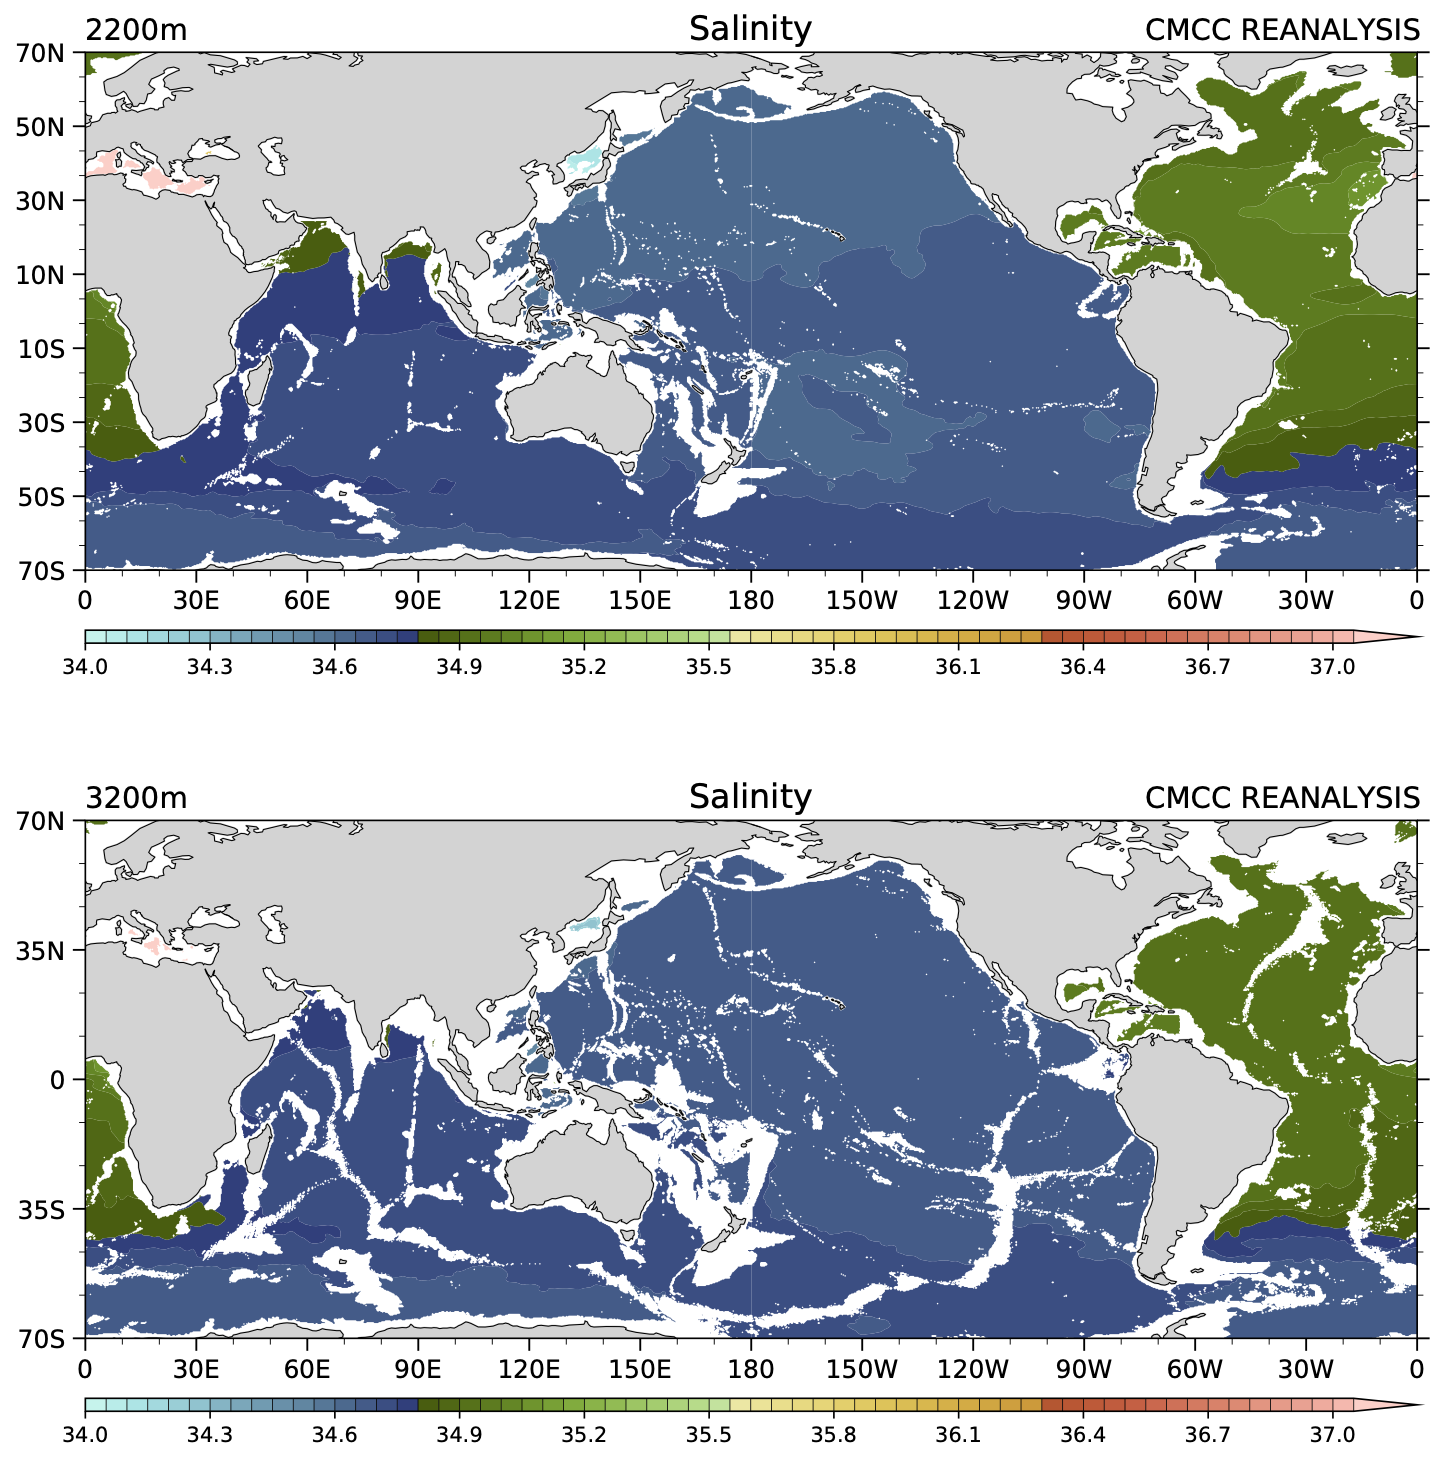
\includegraphics[width = .7 \textwidth]{figs/GD/Sal2200-3200.png}
\caption{} \label{fig:}
\end{figure}

Going even deeper (Fig. \texttt{fig:712}) we have to change drastically
the scale. The oceans are remarkably uniform and the salinity deviations
are really small.

\begin{figure}
\centering
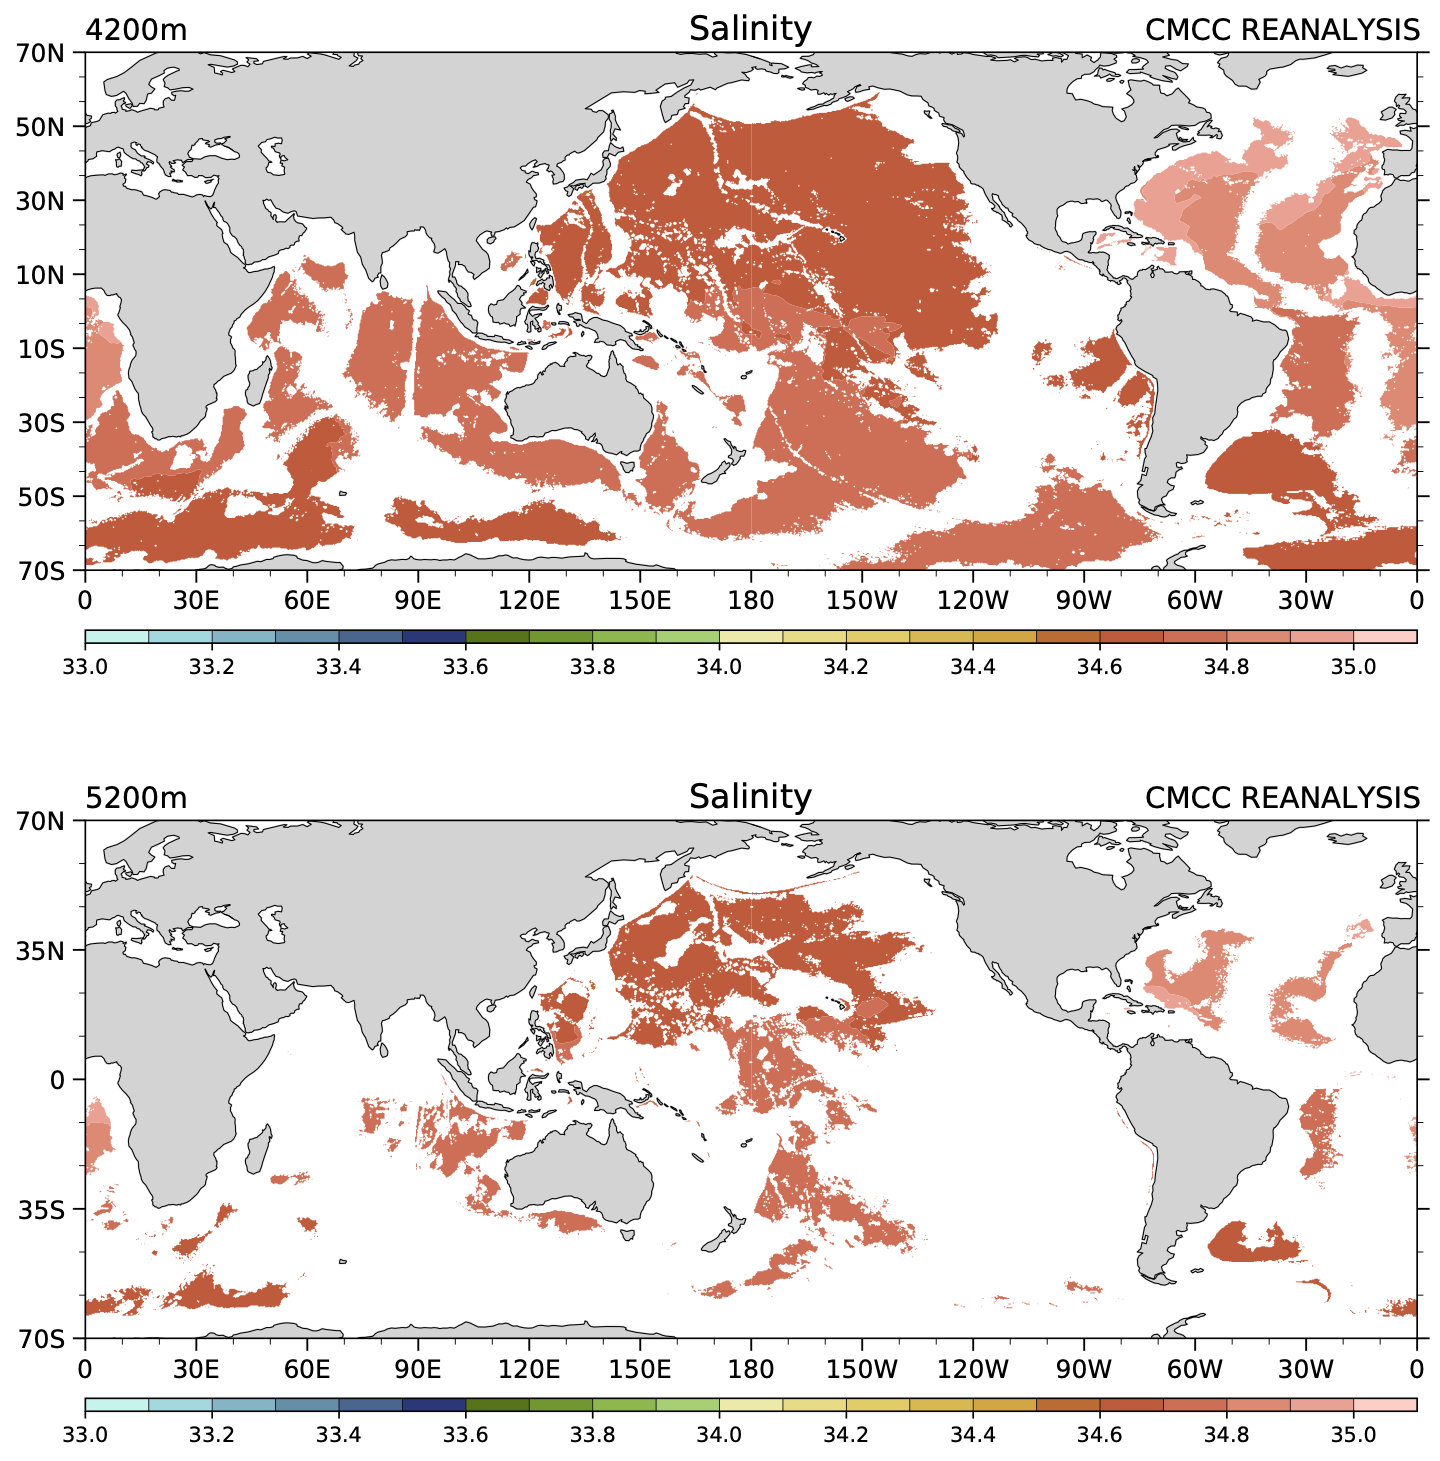
\includegraphics[width = .7 \textwidth]{figs/GD/Sal4200-5200.png}
\caption{} \label{fig:}
\end{figure}

Looking at the North Atlantic (Fig. \texttt{fig:713}) we notice that
there is a strong salinity gradient along the North American Coast that
follows roughly the pattern of the temperature gradient in Fig.
\texttt{fig:613}. Strong temperature gradients are presumably to be
connected to the existence of currents, but we will need to check the
density, depending on the salinity later, to be really sure. Anyway,
this picture is giving a strong indication of the existence of something
remarkable and intense along the western boundary of the Atlantic ocean.

\begin{figure}
\centering
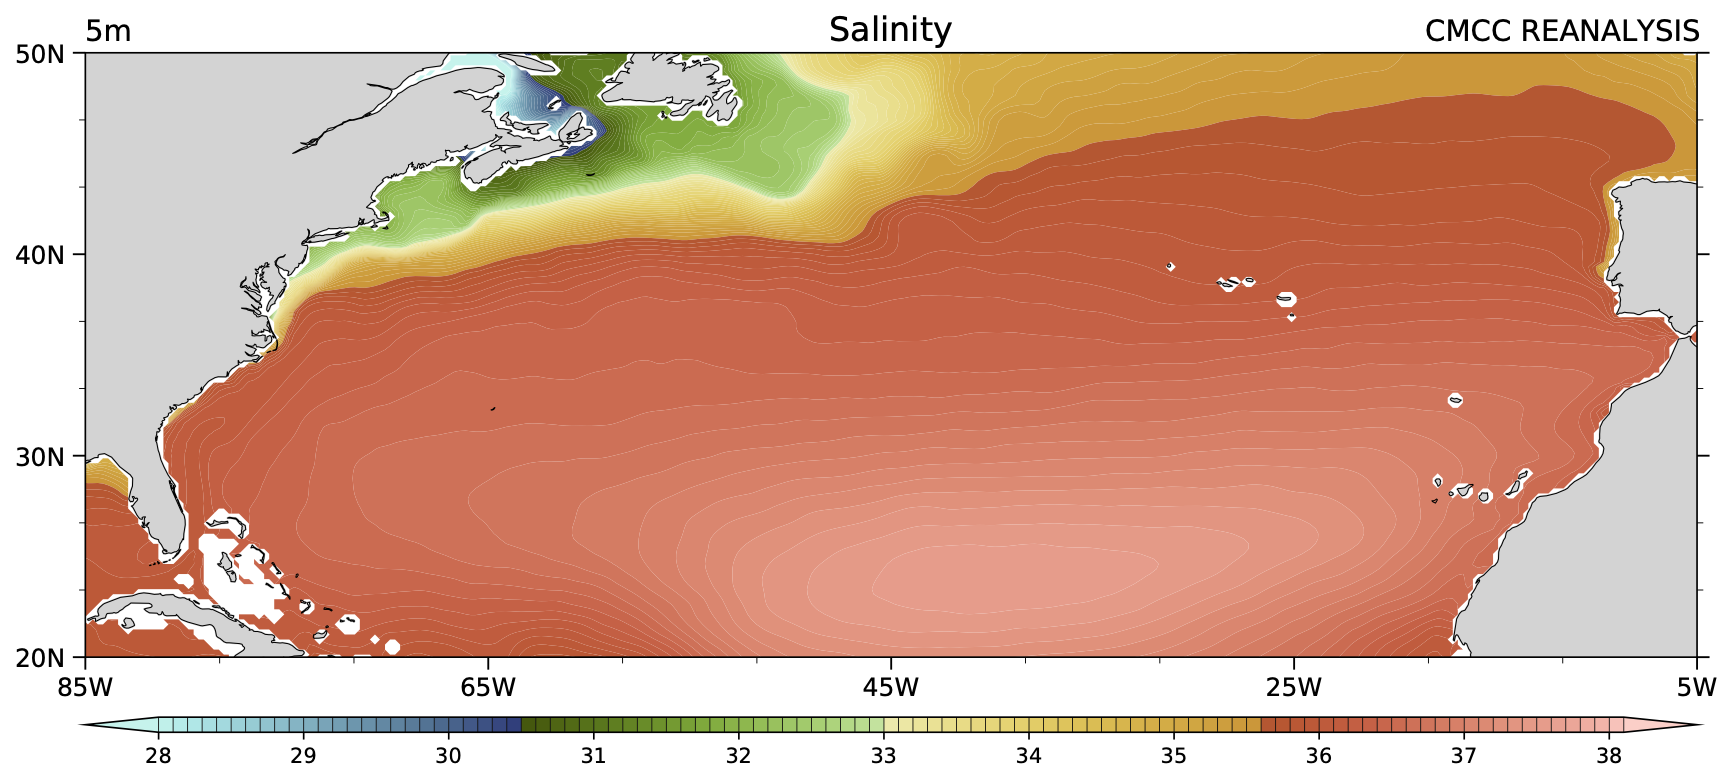
\includegraphics[width = .7 \textwidth]{figs/GD/SGulf5.png}
\caption{Northern Atlantic salinity for the ocean at 5m.}
\end{figure}

A similar situation exist in the North Pacific along the Japan coast and
therefore we can start to suspect that this has to do with the presence
of the continental boundary.

\begin{figure}
\centering
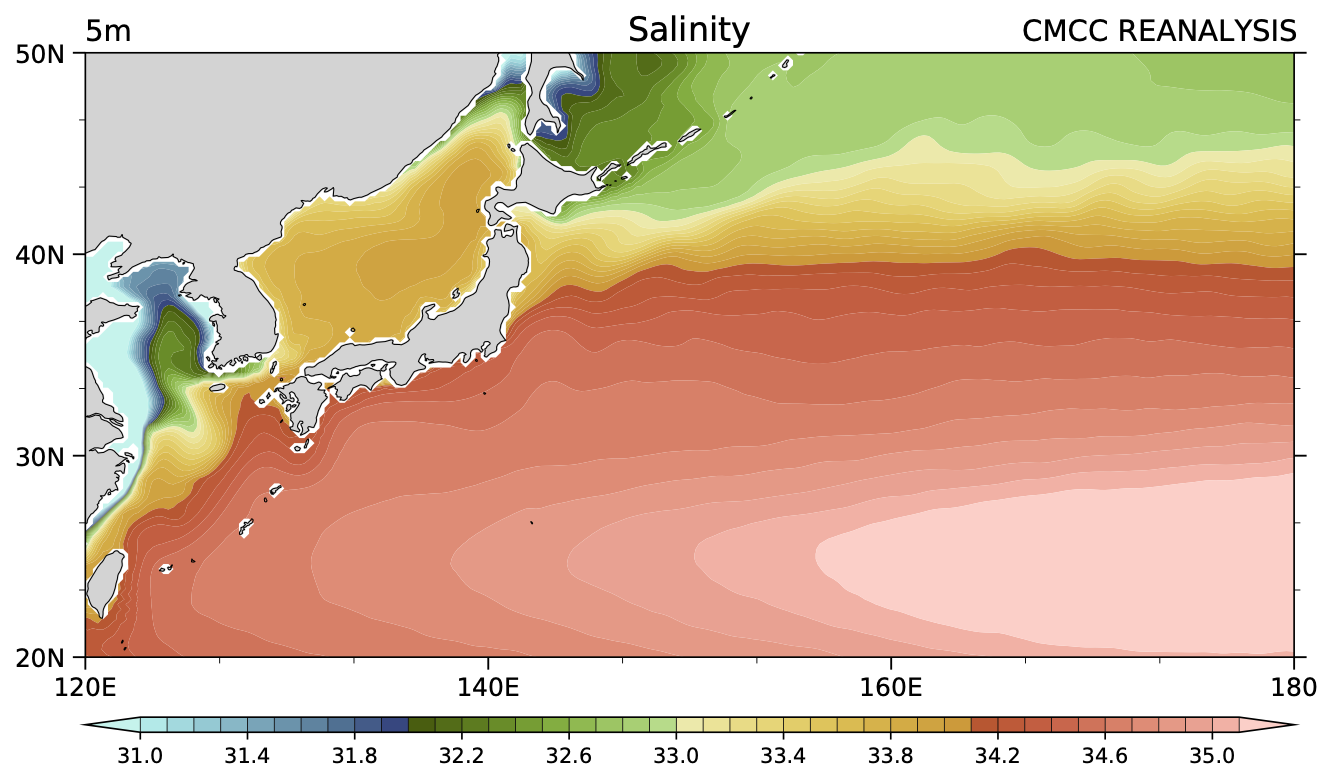
\includegraphics[width = .7 \textwidth]{figs/GD/SKur5.png}
\caption{Northern Pacific Salinity for the ocean at 5m.}
\end{figure}

The previous analysis of the temperature is giving us hints of a strong
vertical structure of the oceans, so it may be useful to look at the
vertical distribution somewhat more in detail. Fig. \texttt{fig:7100}
shows the same section North-South section of Fig. \texttt{fig:6100}
along the longitude of 25W, roughly in the middle of the Atlantic Ocean.
The salinity follows the a similar pattern as the temperature with a
strong gradient approximately at the thermocline, the high salinity is
confined in thin ;layers at the surface, but some interesting behaviour
is visible below. In the Northern Hemisphere we can see the
Mediterranean water penetrating at depth and actually protruding under
the fresher water of Antarctic origin that is colder, but because is
fresher floats over the Mediterranean water. Really cold Antarctic water
reaches the bottom, filling the abyssal plains of the basin.

\begin{figure}
\centering
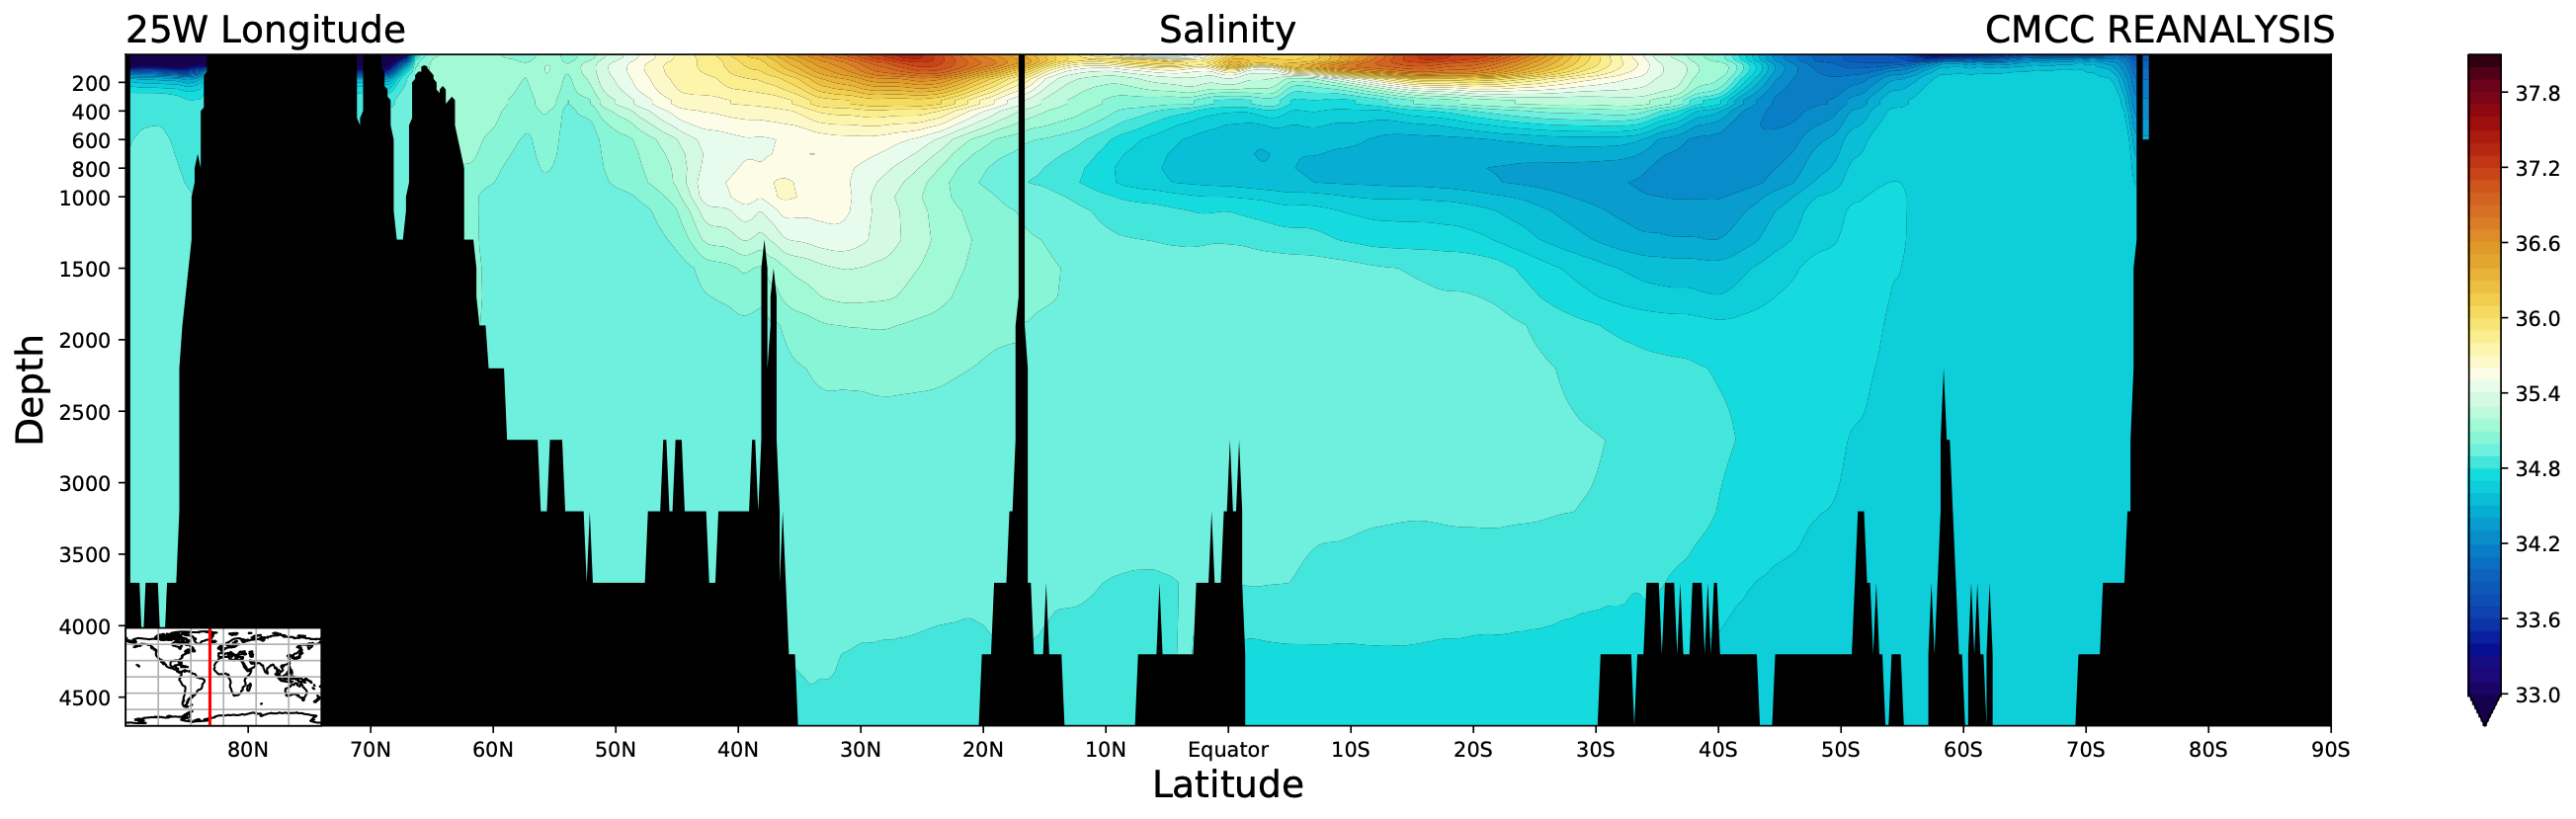
\includegraphics[width = .7 \textwidth]{figs/GD/SectSal25W5000.png}
\caption{North-South Salinity section at 25W longitude.}
\end{figure}

The Mediterranean waters are clearly visible in a longitude-depth
section (Fig. \texttt{fig:71000}). The saline mediterranean water sinks
to about 1000m because it is warmer than the Atlantic but much more
saline so it is denser and it reaches an equilibrium depth at about
1000m.

\begin{figure}
\centering
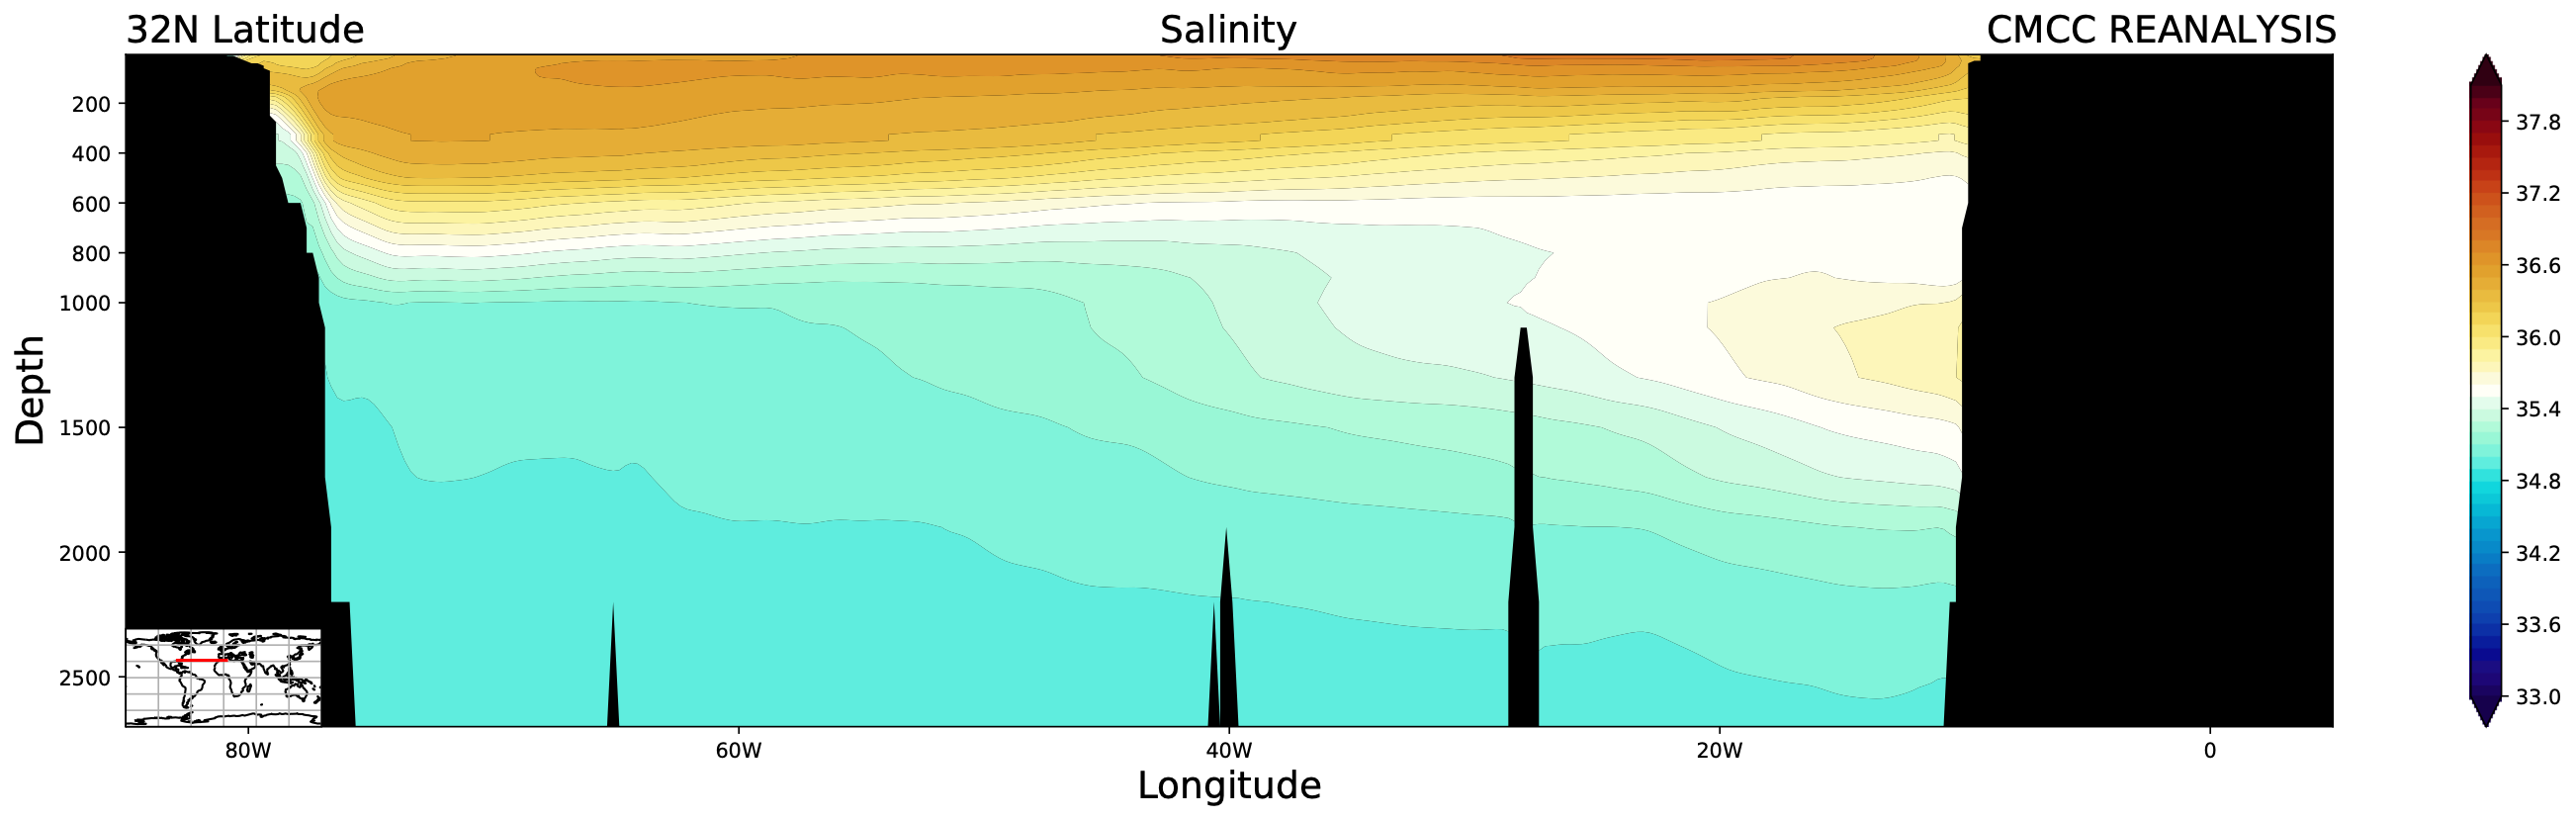
\includegraphics[width = .7 \textwidth]{figs/GD/SectSalinity32N3000.png}
\caption{Longitude depth section about 32N in the Atlantic Ocean.}
\end{figure}

\begin{figure}
\centering
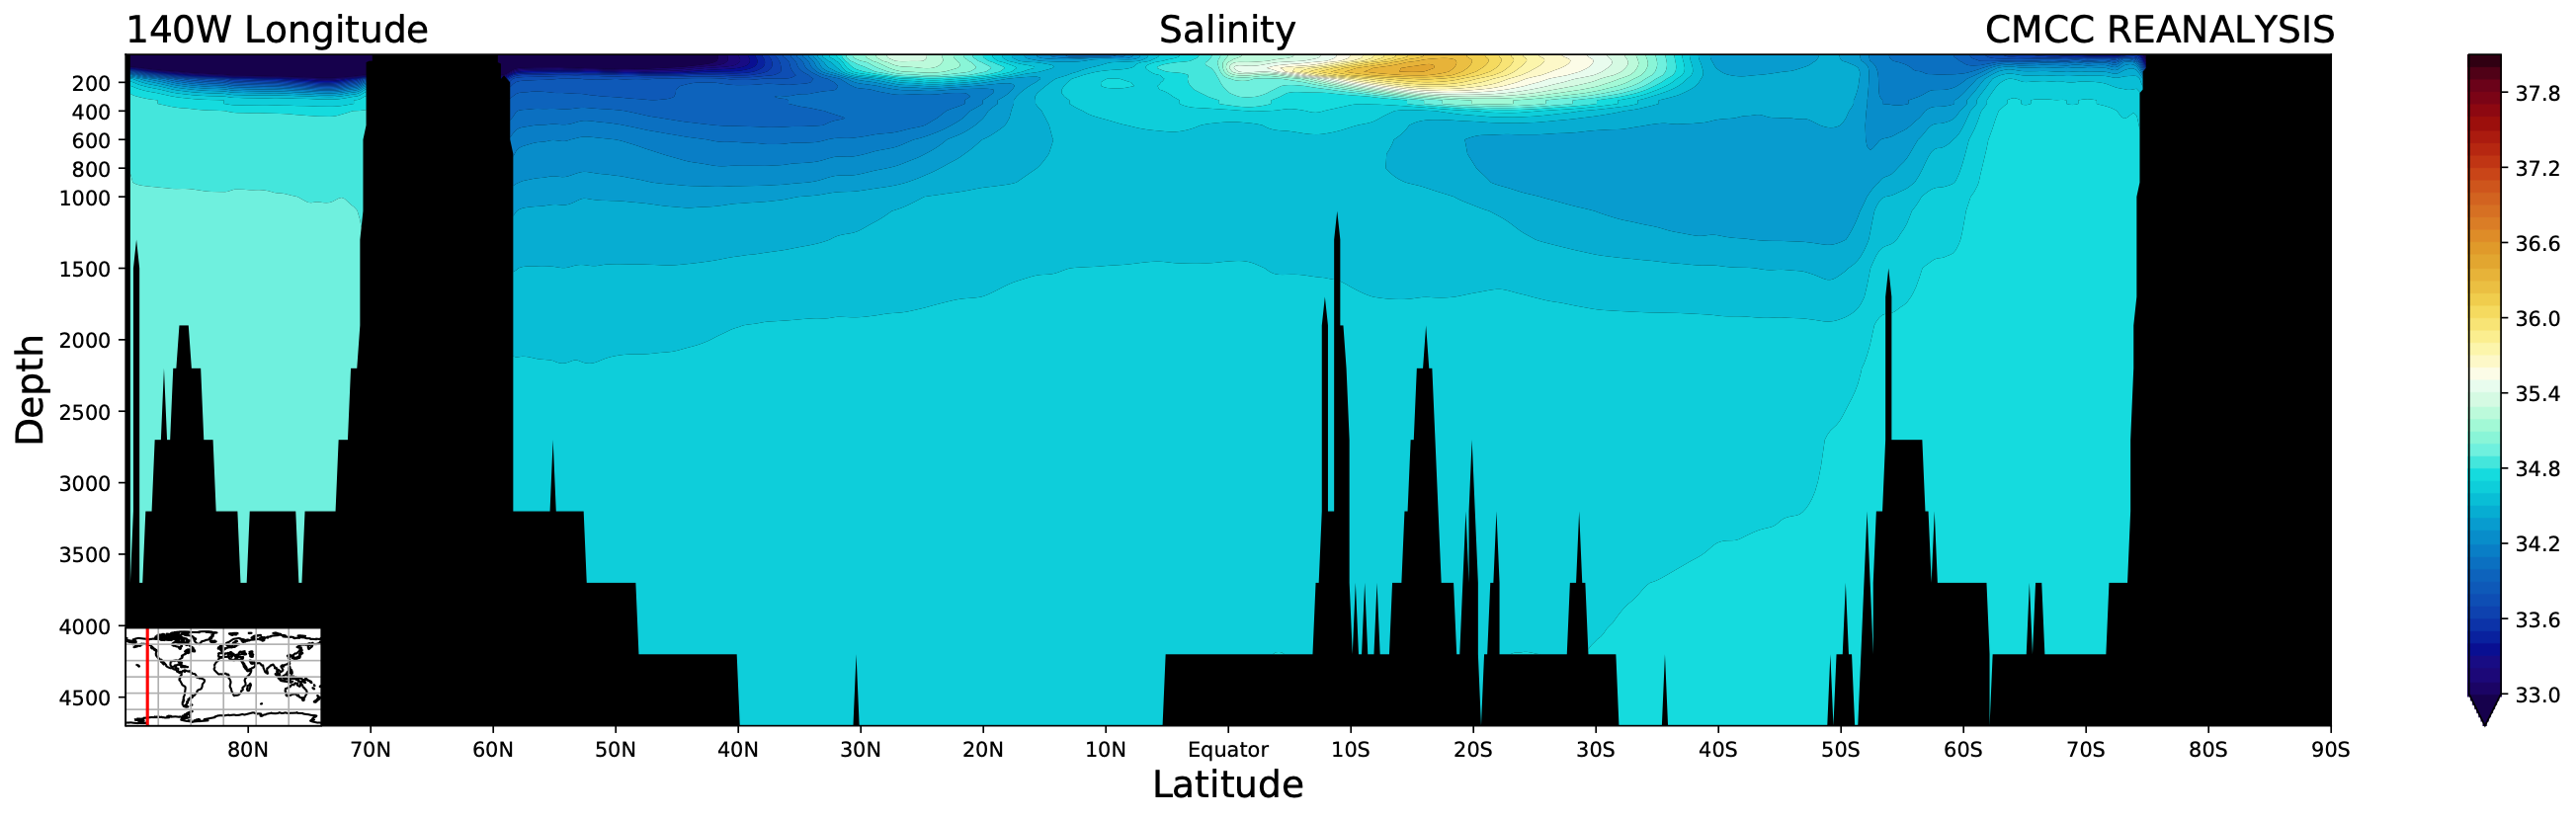
\includegraphics[width = .7 \textwidth]{figs/GD/SectSal140W5000.png}
\caption{As in Fig. \texttt{fig:7100} but for 140W longitude}
\end{figure}

The vertical structure of the Pacific Ocean (Fig. \texttt{fig:7101}) is
different and what we see is a situation where salinity is slowly
varying getting fresher toward the surface, with the thin saline water
in the subtropics a clear signature of the equatorial upwelling and the
Antarctic water filling the abyssal plains. The Indian Ocean is similar
to the Pacific South of the Equator but North of the Equator at this
longitude is fresher.

\begin{figure}
\centering
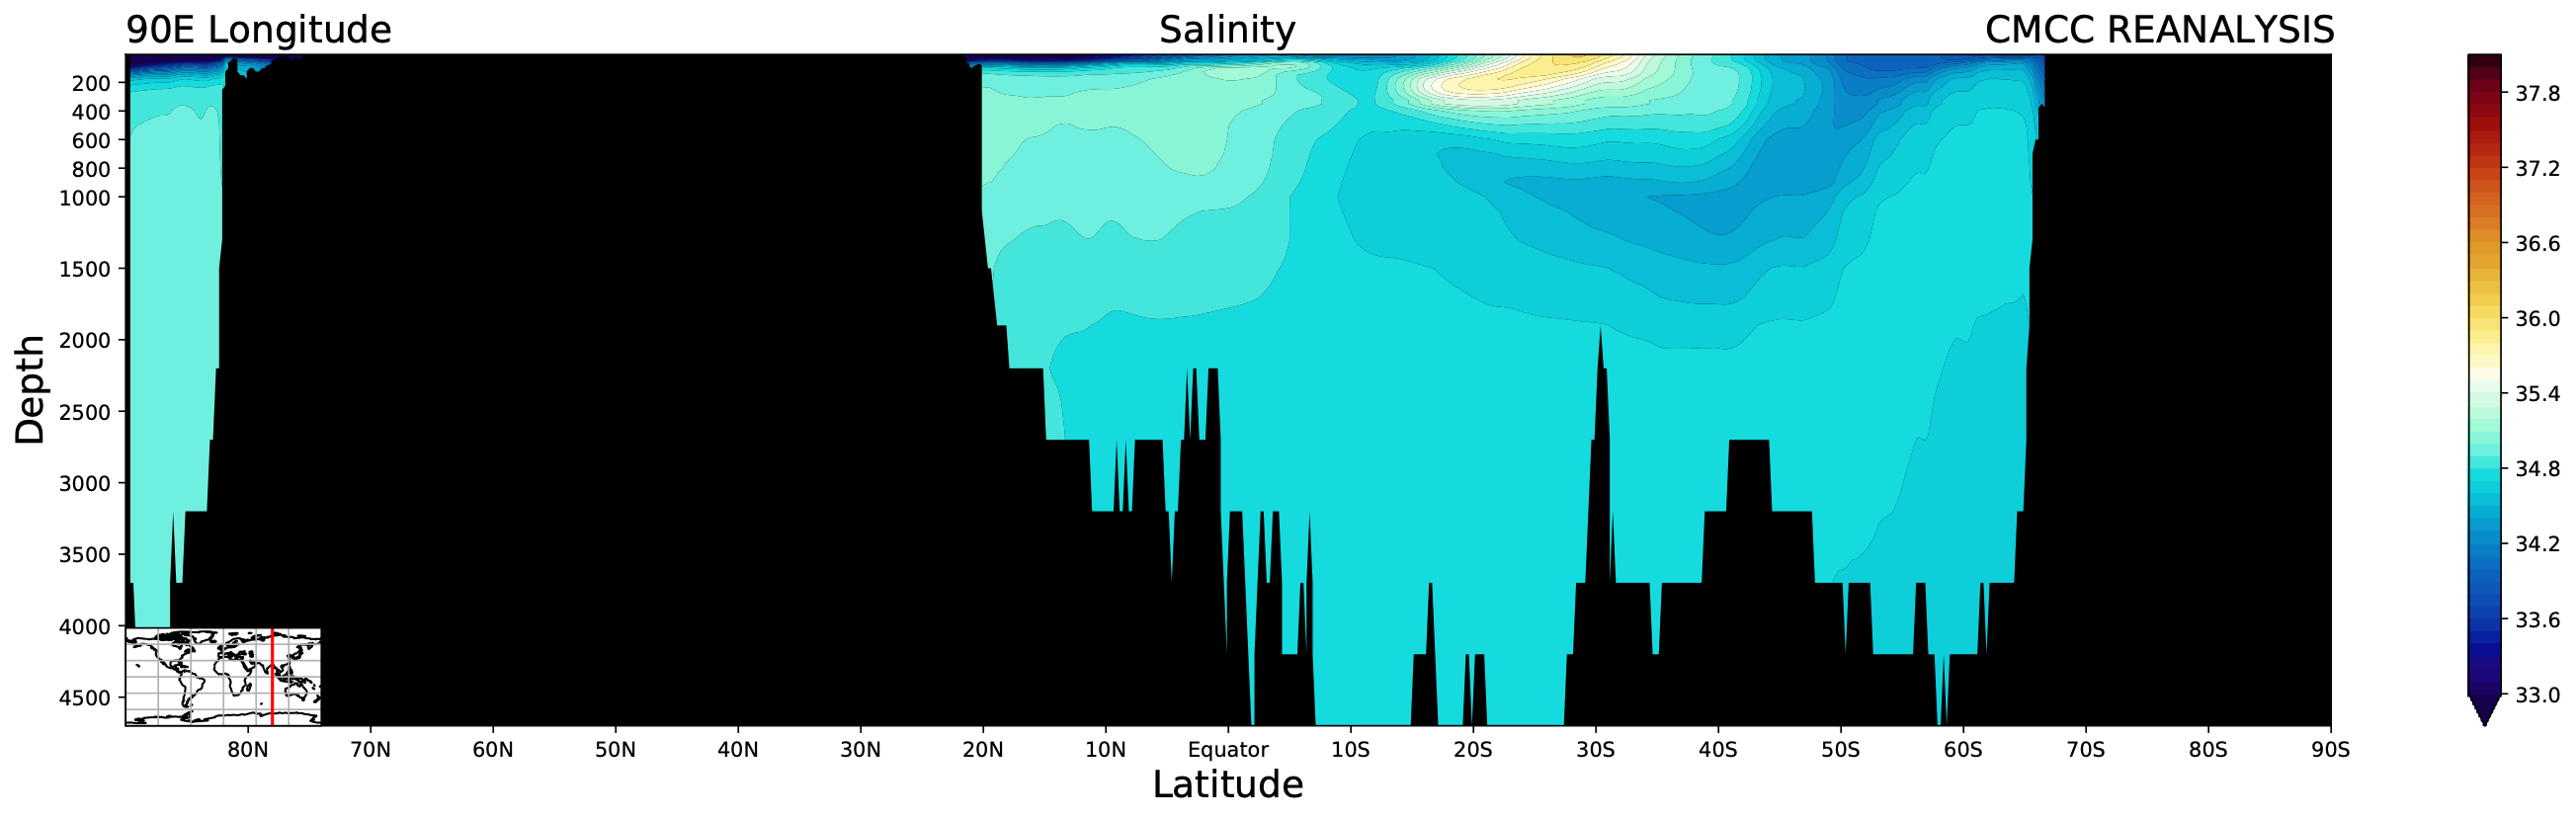
\includegraphics[width = .7 \textwidth]{figs/GD/SectSal90E5000.png}
\caption{As in Fig. \texttt{fig:7100} but for 90E longitude}
\end{figure}

The Indian Ocean (Fig. \texttt{fig:7102}) shown here as a section
cutting essentially through the Bay of Bengal, shows a similar strong
stratification, but there are only weak signs of an equatorial upwelling
of cold water.

\begin{figure}
\centering
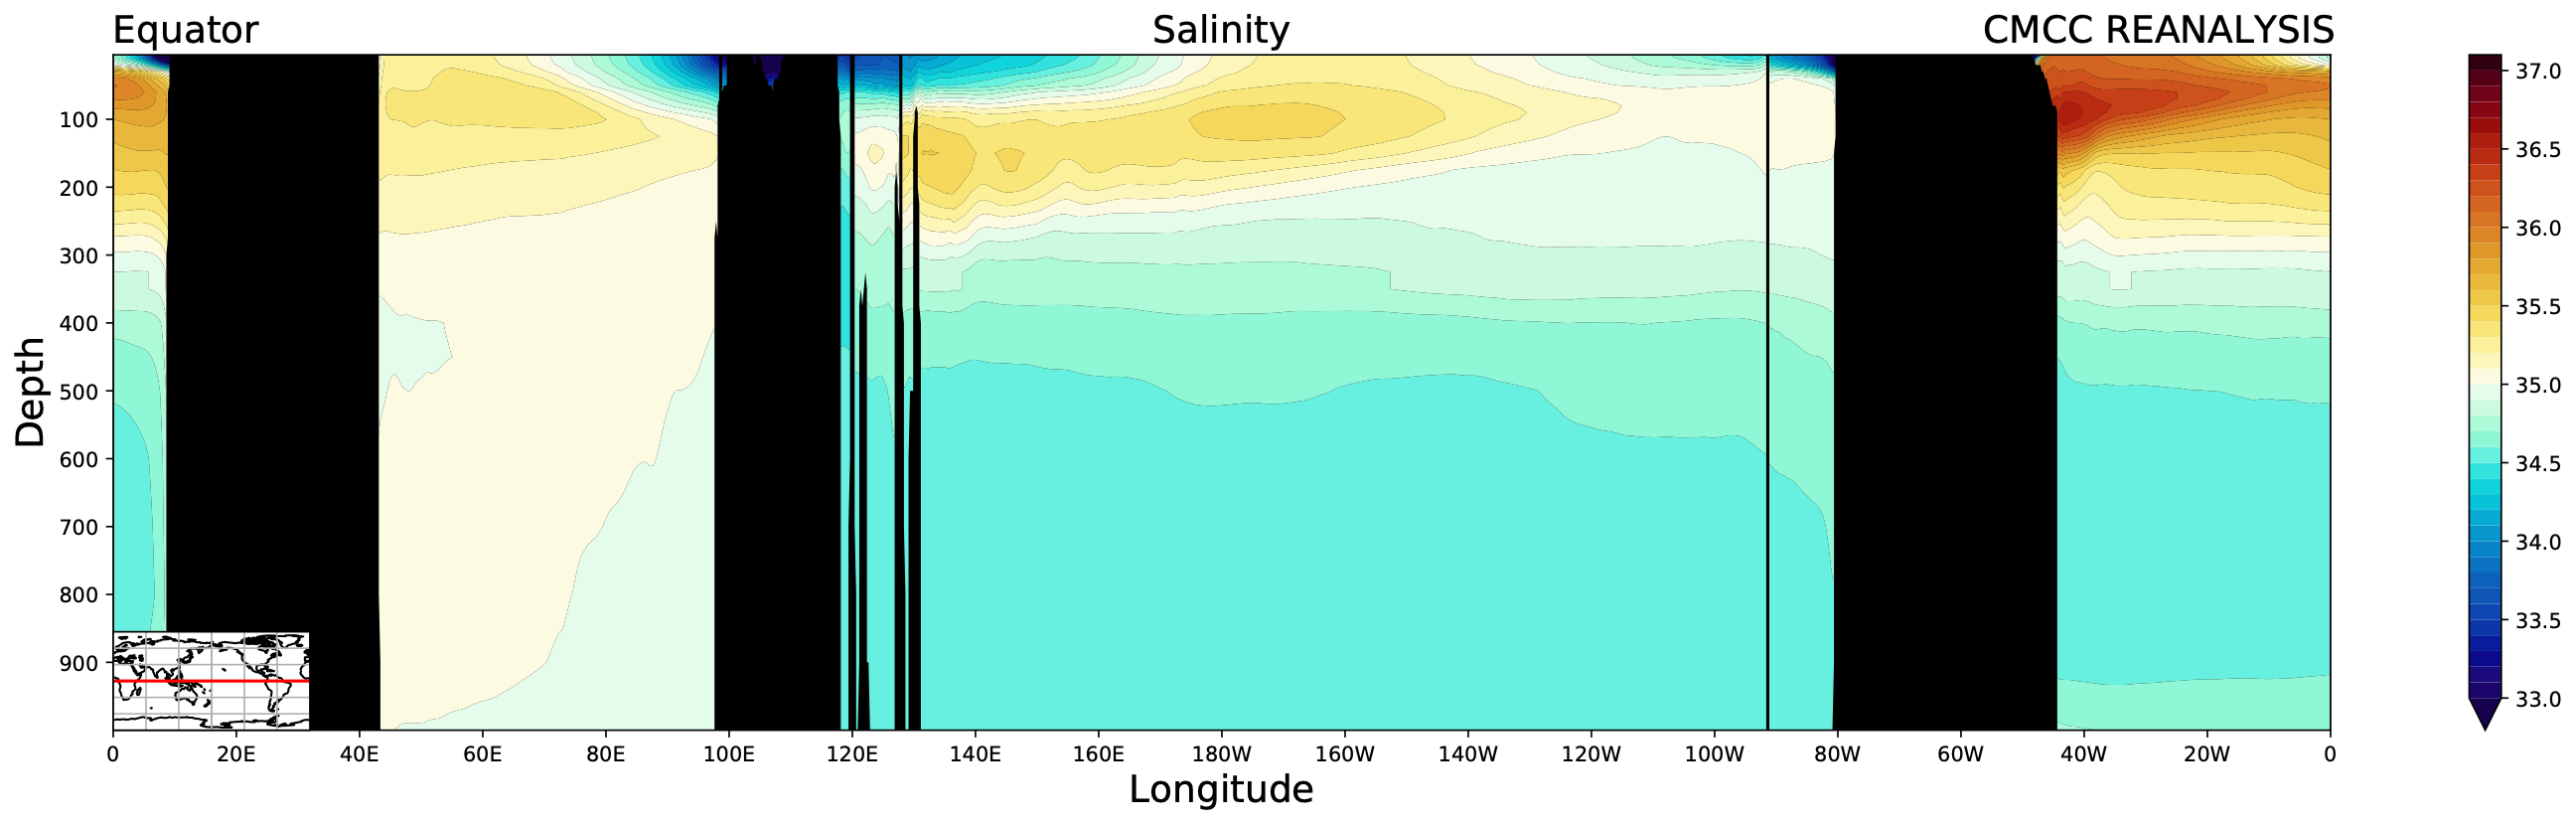
\includegraphics[width = .7 \textwidth]{figs/GD/SectSalinityEquator1000.png}
\caption{} \label{fig:}
\end{figure}

We can gain more insights in the equatorial structure by looking at a
longitudinal section along the Equator in the Pacific (Fig.
\texttt{fig:7103}). Here we see the general difference between the
Atlantic and the Pacific, but we also see that the salinity is following
the slant of the equatorial thermocline and the equatorial upwelling in
the East Pacific. The effect of the major precipitation center of ITCZ
in the West Pacific is visible in fresh water at the surface in the
West.

\subsection{Ocean Currents}\label{ocean-currents}

\subsubsection{The overall basin
circulation}\label{the-overall-basin-circulation}

The surface currents of the Atlantic ocean are shown in Fig.
\texttt{fig:8100}. As we might have suspected from the temperature
structure there is a strong northward current along the North American
coast that reaches all the way across the North Atlantic to Europe, the
Gulf Stream. Strong currents are also visible in the Equatorial area
where they connect to the mid-latitude circulation forming a large
circular system, the Subtropical Gyre. The South Atlantic has a similar
gyre in the subtropical region, but at higher latitudes we can notice a
strong westerly current cutting all along the basin, essentially along a
latitude line between 40S and 50S.

\begin{figure}
\centering
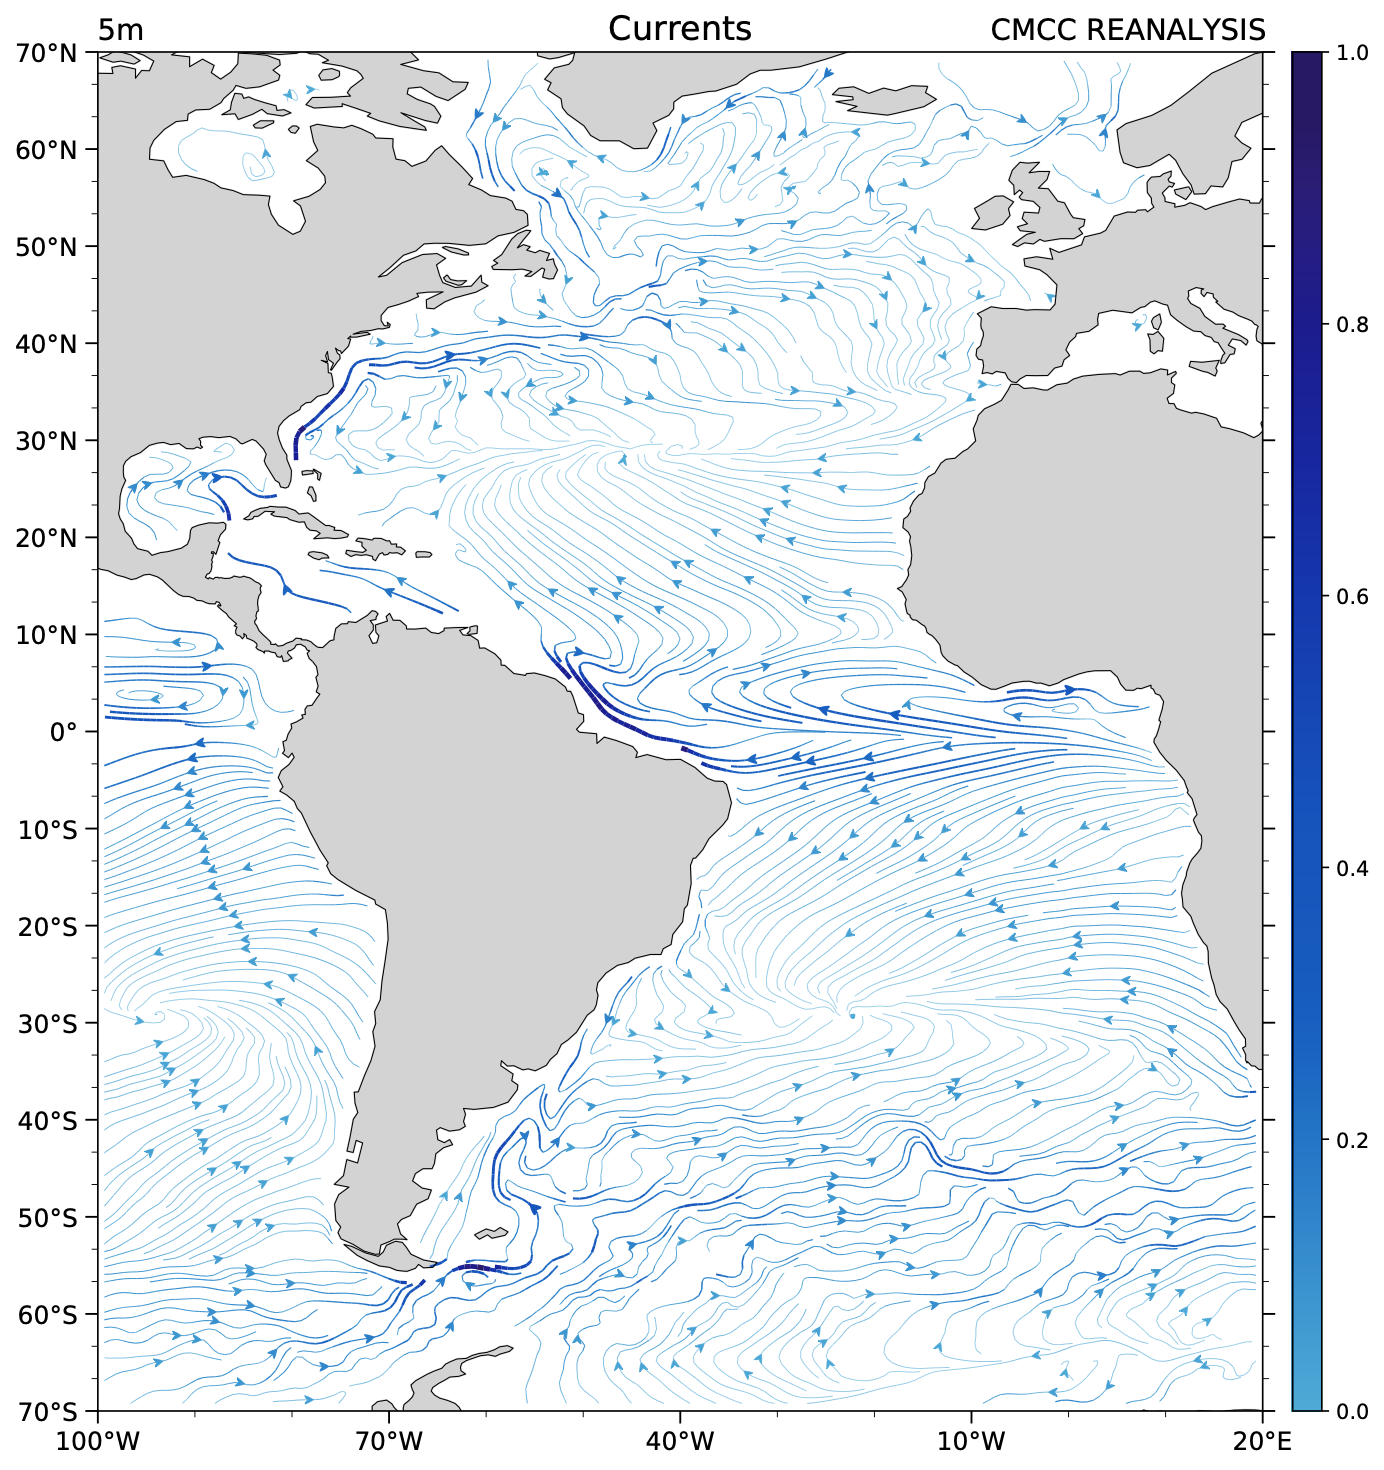
\includegraphics[width = .7 \textwidth]{figs/GD/UVstream5mGLOBNA.png}
\caption{} \label{fig:}
\end{figure}

The North Pacific surface circulation is shown in Fig.
\texttt{fig:8101}. We can notice here again a strong current along the
Western boundary of the basin that than feed into a basin wide gyre that
connects to the equatorial circulation. The boundary current, known her
as the Kuroshio Current, is very narrow and intense along the Japan
coast, as it is also the case of the Gulf Stream in the Atlantic, and it
tapers into a wide system of streams and eddies into the open ocean.

It is possible to see also local system, like the small gyre off the
Alaskan coast and similar circulation in the marginal seas, like the Sea
of Okhotsk, near the Siberian coast. Their presence is remarkable as we
are looking here at climatological averages over more than 40 years and
so they are stable and persistent features. This is another reminder of
how even relatively smaller feature in the ocean can be climatologically
persistent over many years.

\begin{figure}
\centering
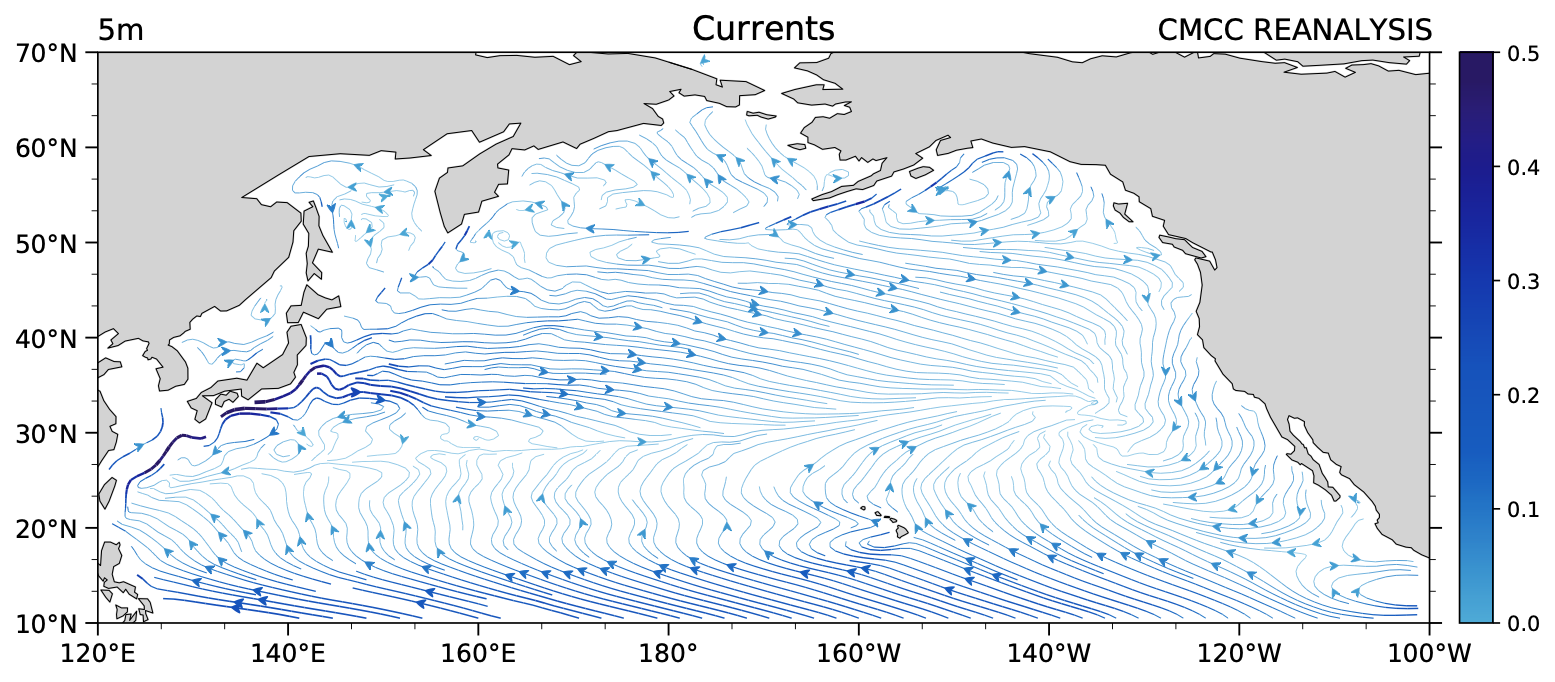
\includegraphics[width = .7 \textwidth]{figs/GD/UVstream5mGLOBNP.png}
\caption{} \label{fig:}
\end{figure}

The circulation of the South Pacific Ocean is shown in Fig.
\texttt{fig:8102}. The subtropical gyre is visible also here, but there
is a weak indication of a western intensification current in the West
pacific, close to the coasts of Australia and New Zealand. The strong
high latitude current that we have seen in the Atlantic is aldo present
here end evidently connect to the other basin through the Drake Passage,
that is the Straits between South America and Antarctica.

\begin{figure}
\centering
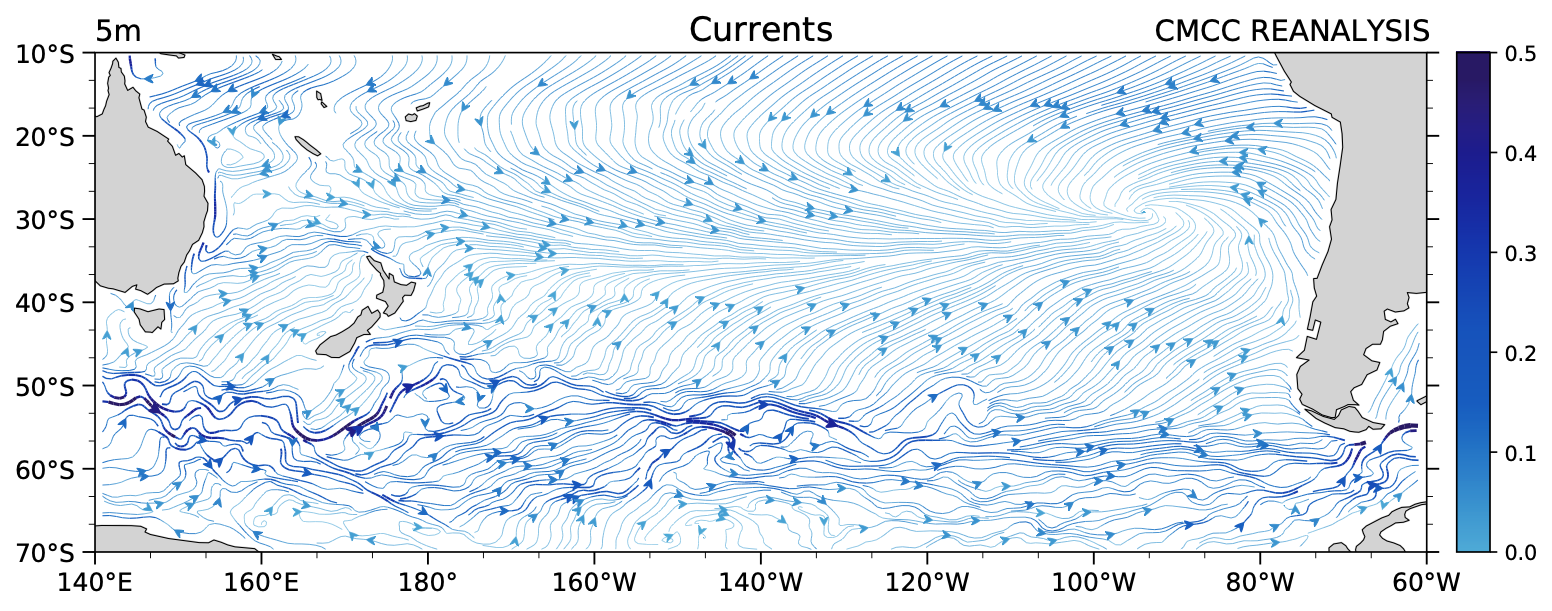
\includegraphics[width = .7 \textwidth]{figs/GD/UVstream5mGLOBSP.png}
\caption{} \label{fig:}
\end{figure}

The Indian Ocean circulation is shown in Fig. \texttt{fig:8103}. The
Indian Ocean is confined by continental masses in the north, so it is
mostly composed of the equatorial region and the midlatitudes are all in
the Southern Hemisphere. The subtropical gyre is present, together with
features North of Madagascar. A boundary current develops on the African
coast, The westerly current in the southern mid-latitudes is visible
also here, strong and with a vigorous eddy field.

\begin{figure}
\centering
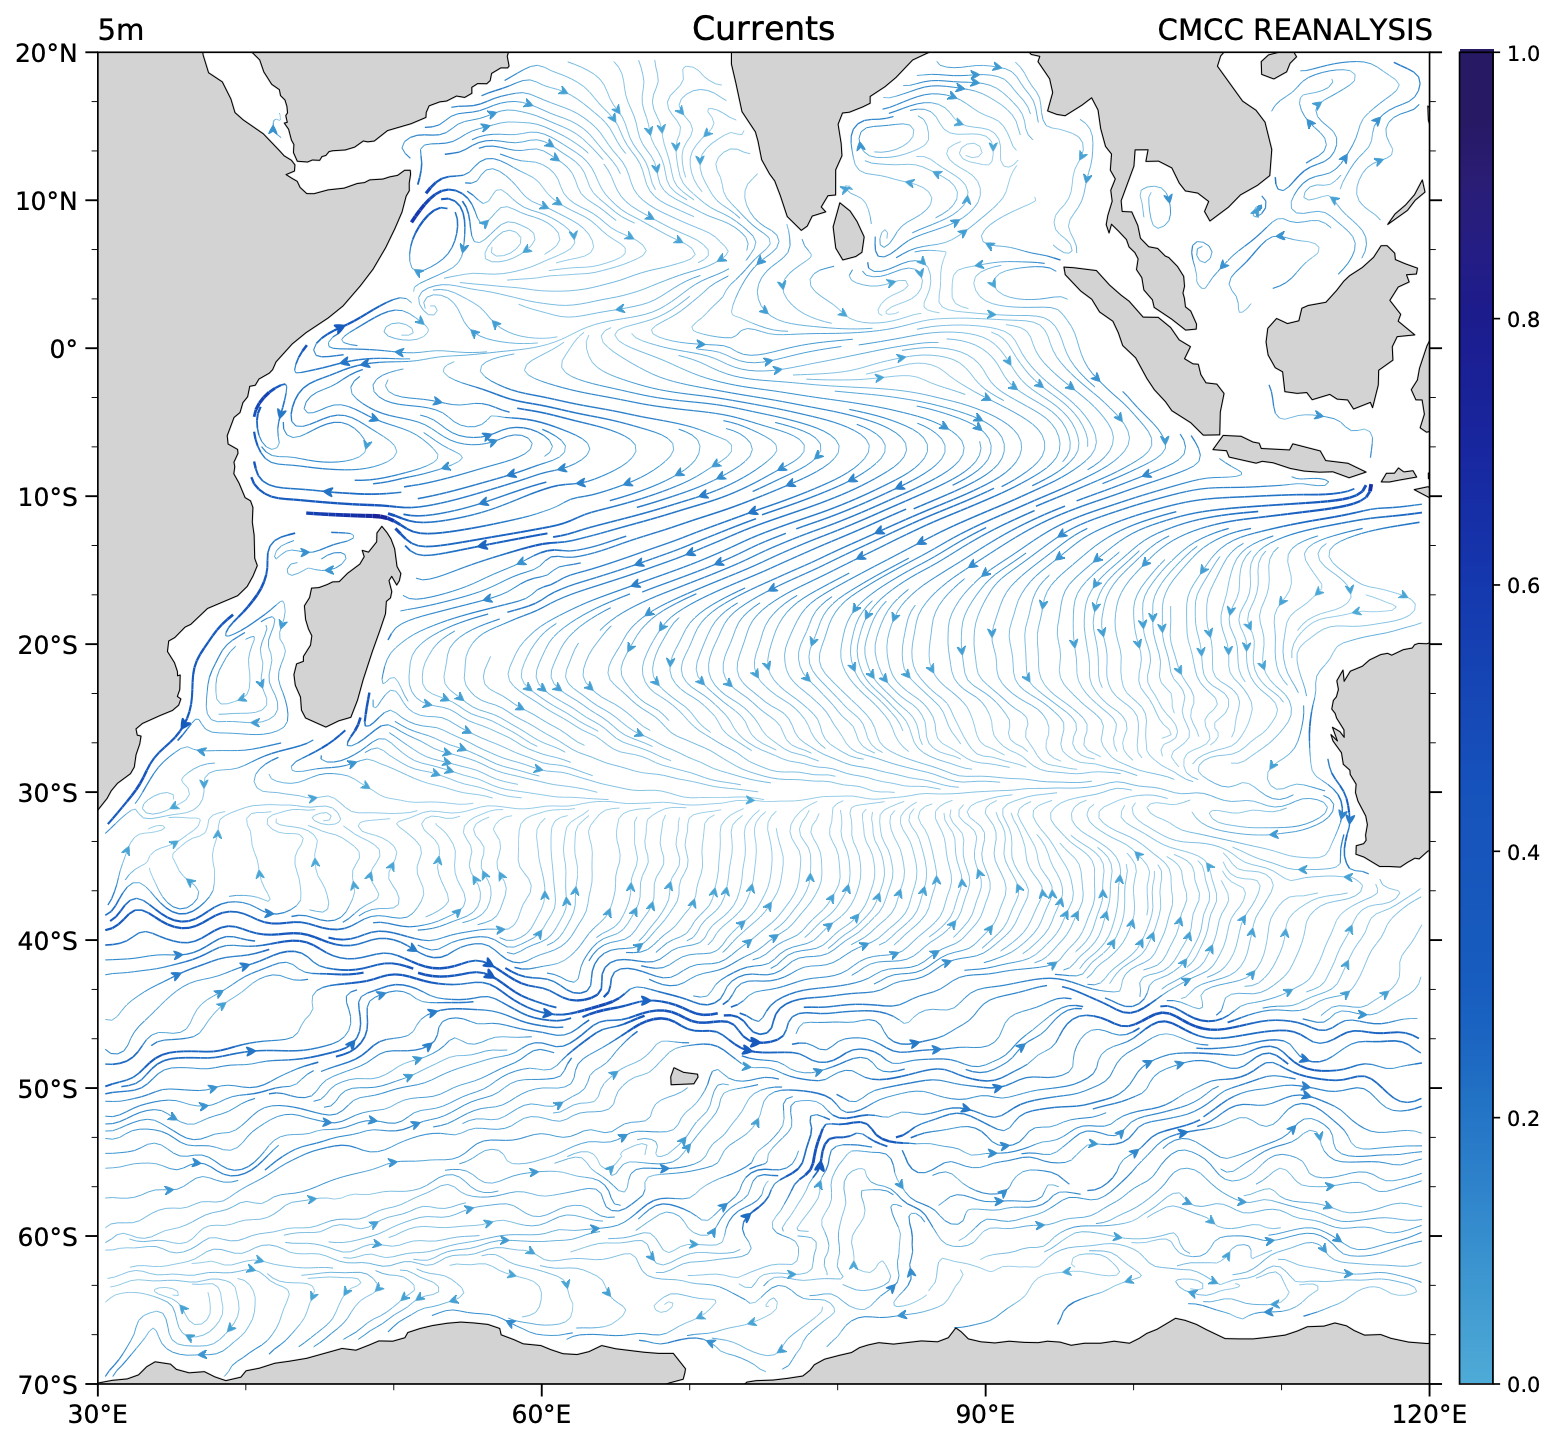
\includegraphics[width = .7 \textwidth]{figs/GD/UVstream5mGLOBIND.png}
\caption{} \label{fig:}
\end{figure}

At this point we can suspect that there is probably a continuous ring of
currents around Antarctica and this can be confirmed by the bottom panel
of Fig. \texttt{fig:8103} that shows the entire extent around a
longitude circle of the current, known as the Antarctic Circumpolar
Current. It is a strong, highly turbulent system that connects all the
Ocean Basins.

\subsubsection{The equatorial
circulation}\label{the-equatorial-circulation}

The Equator is a special place for the atmosphere and so it is a special
place also for the Oceans. The circulation in this area is strongly
coupled with the atmospheric circulation and it is often characterized
by both westerly and easterly currents and by special behaviours right
at the Equator line. Futhermore, it is also very different from ocean to
ocean.

The equatorial current system in the Pacific Ocean is shown in Fig.
\texttt{fig:8106}. It is a complex system composed of two easterly
currents, the North and South Equatorial currents, sandwiching the
westerly Equatorial countercurrent. It is possible to notice that at the
Equator the currents are strongly easterly and diverging, leading to the
emergence of upwelling at the Equator by Ekman transport.

\begin{figure}
\centering
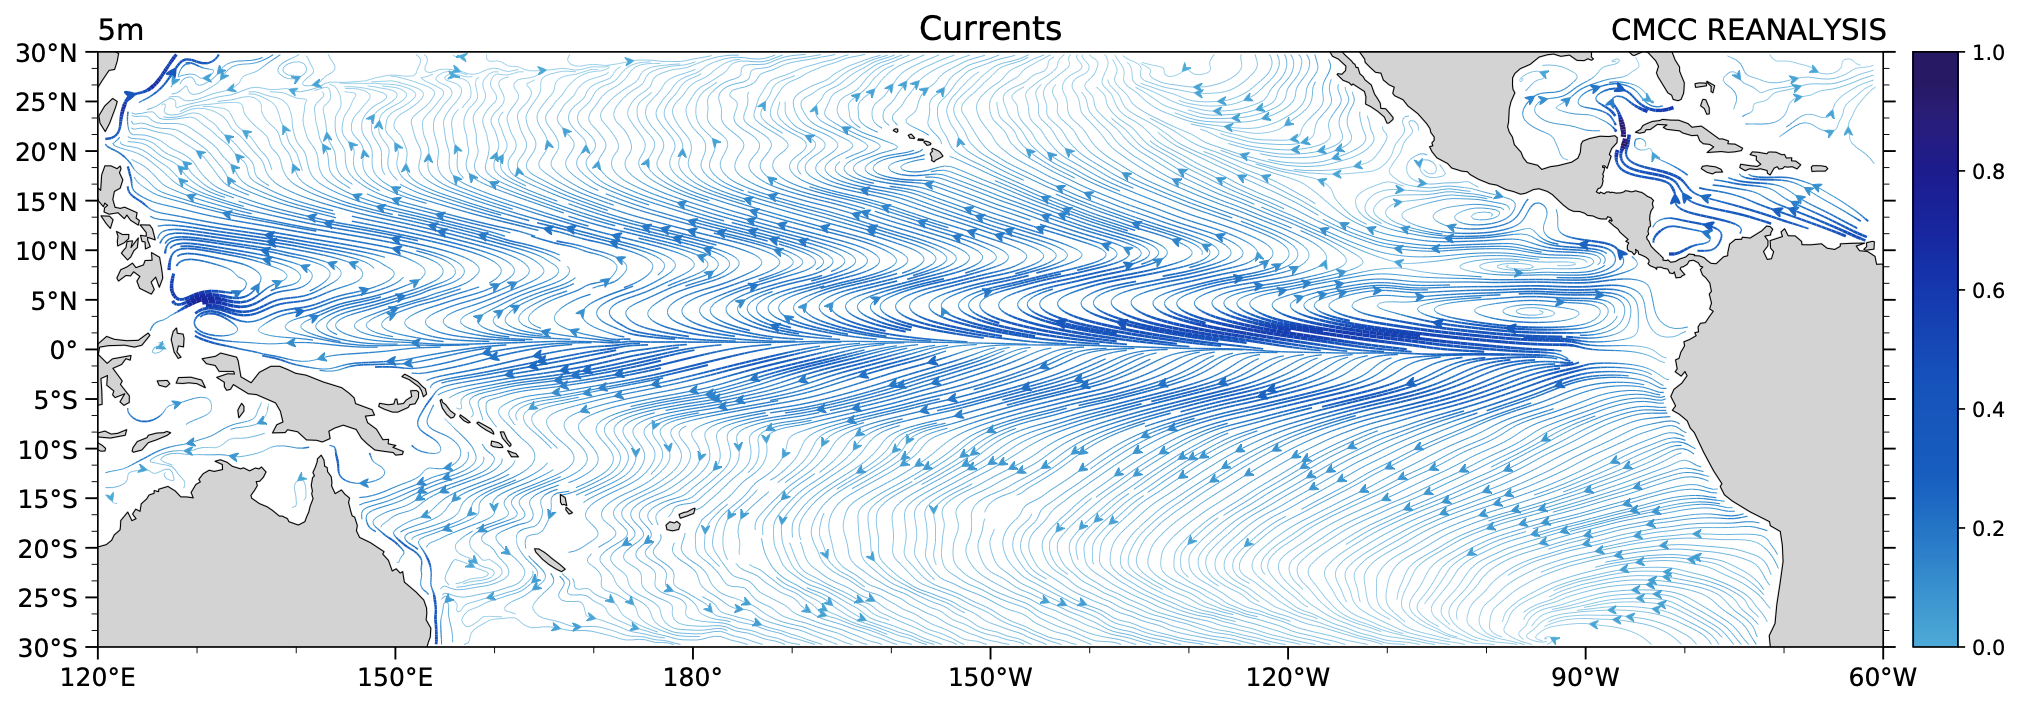
\includegraphics[width = .7 \textwidth]{figs/GD/UVstream5mPac.png}
\caption{} \label{fig:}
\end{figure}

The complexity of the equatorial current system can be further
appreciated by looking at the vertical section of the zonal current at
the Equator (Fig. \texttt{fig:8107}) A strong westerly current below the
surface, slanting from the West Pacific to the East Pacific, is visible
at depth between 200 and 300m. The speed is in excess of 1 m/s and it
gets progressively shallower in the East.

It is however part of an alternation of westerly and easterly currents
that become progressively weaker as they get deeper. They are centered
almost perfectly at the Equator, as it can be seen in Fig.
\texttt{fig:8108}. The latitudinal position of the undercurrent is very
tightly controlled by rotational effects and it precisely tracks the
position of the equatorial line.

\begin{figure}
\centering
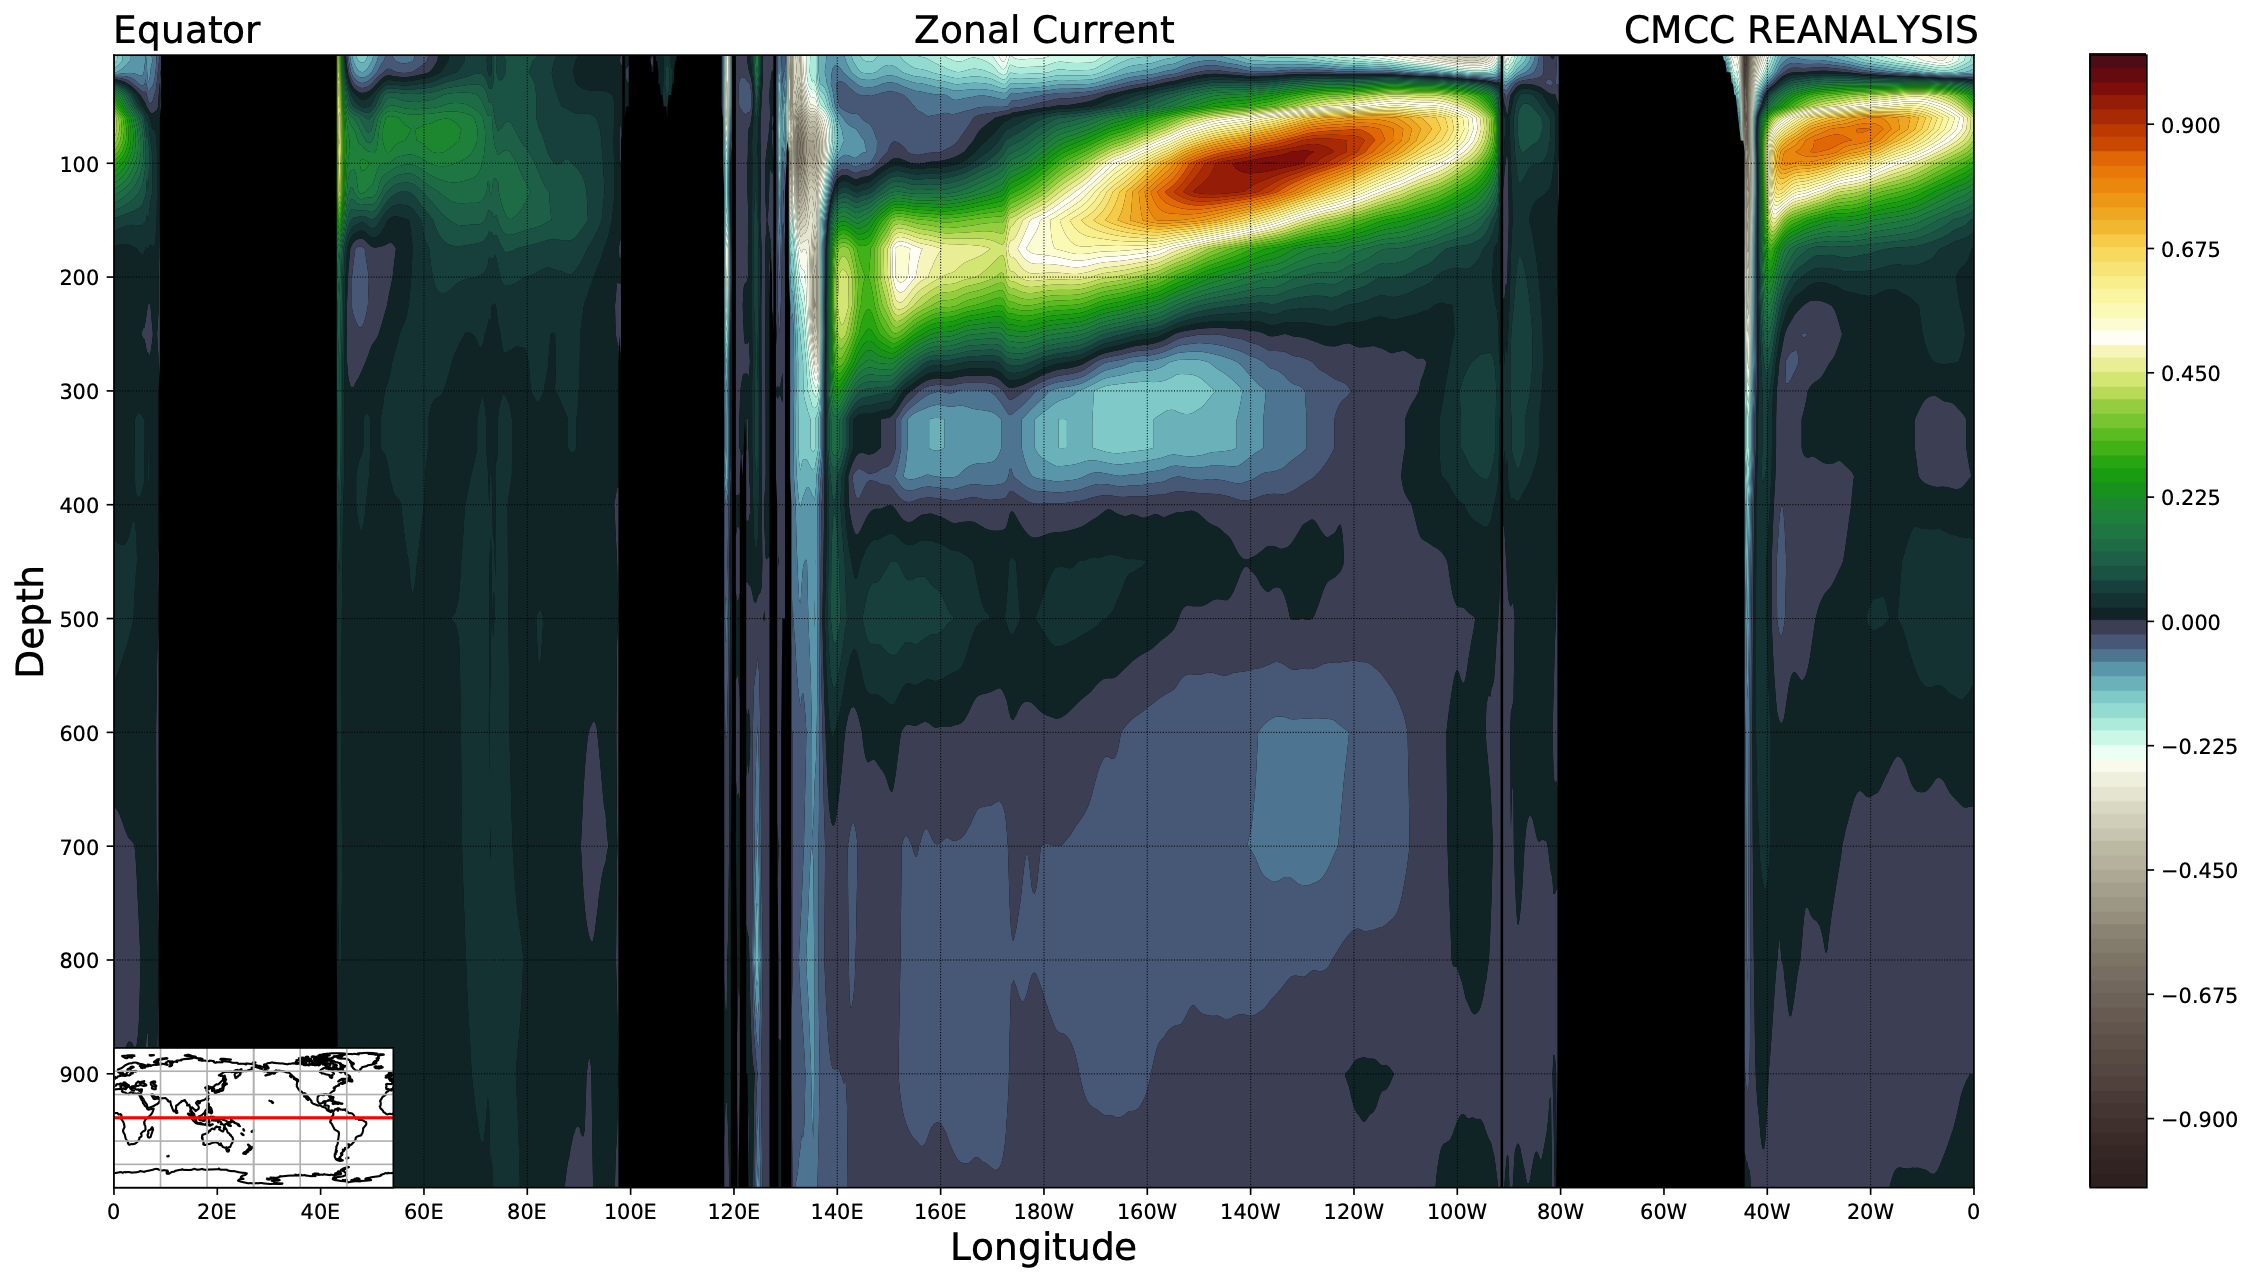
\includegraphics[width = .7 \textwidth]{figs/GD/SectZonal_CurrentEquator1000.png}
\caption{} \label{fig:}
\end{figure}

The equatorial Atlantic Ocean surface circulation (Fig.
\texttt{fig:8109}). It is possible to see the easterly South Equatorial
Current that is straddling the Equator between 5S and 5N. The North
equatorial Countercurrent is westerly and it covers the area between 5N
and 10N, and the weaker North Equatorial Current is located at northern
latitudes. The equatorial flow is divergent and also in this case we can
presume the existence of upwelling at the Equator. A strong coastal
current is visible as the Guinea Current, in the Gulf of Guinea. The
South Equatorial Current feeds into the North Brazilian Current that
then flows northward along the South America coast, taking different
names as it finally emerges as the Caribbean Current in the Caribbean
sea.

A similar structure of alternating westerly and easterly undercurrents
exist also in the equatorial Atlantic (Fig. \texttt{fig:8108}), but it
is weaker and only the first westerly maximum is well visible. It is
also slanting towards the East, but the maximum is reached more towards
the western boundary of the basin with respect to the Pacific Ocean. The
deeper easterly jets are also much less weaker. The undercurrents jets
are essentially absent in the Indian Ocean.

\begin{figure}
\centering
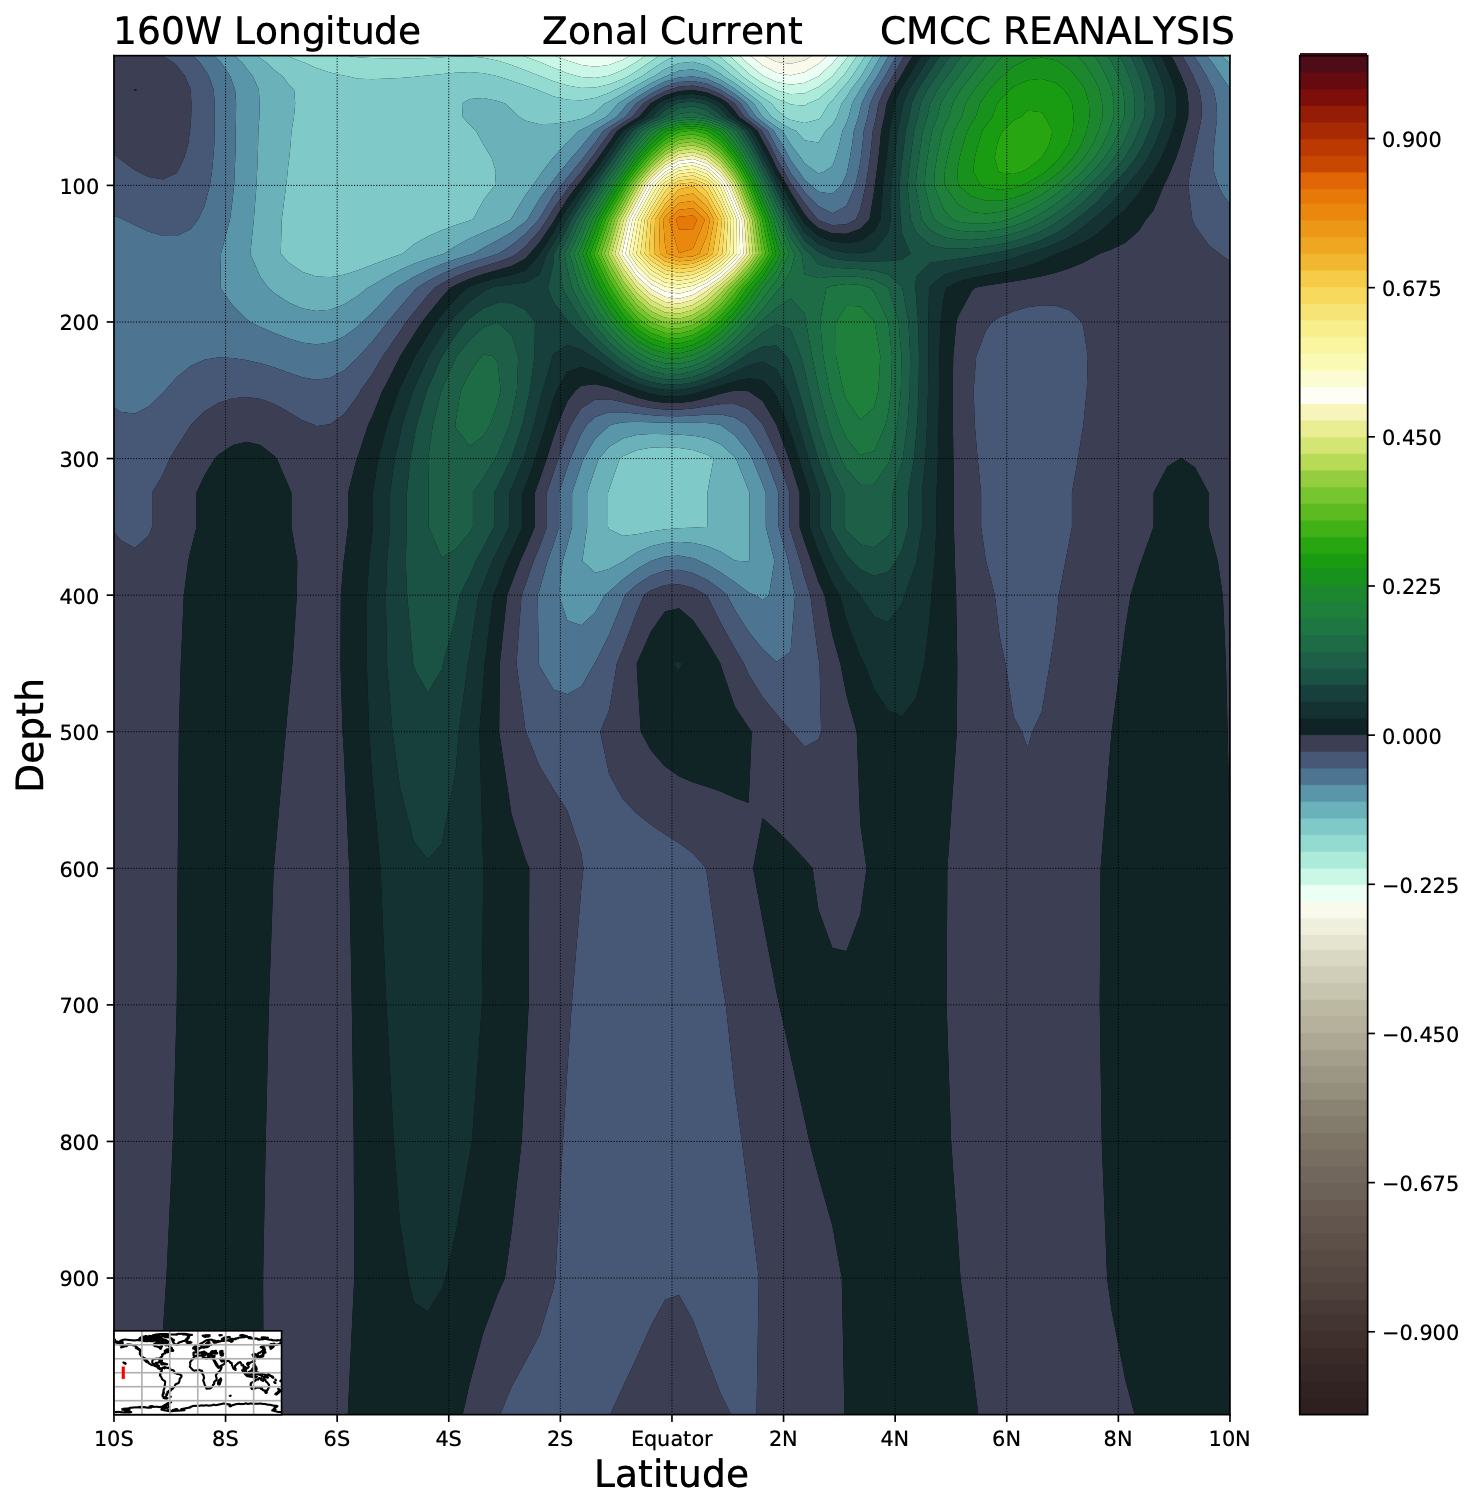
\includegraphics[width = .7 \textwidth]{figs/GD/SectZonal_Current160W1000.png}
\caption{} \label{fig:}
\end{figure}

\begin{figure}
\centering
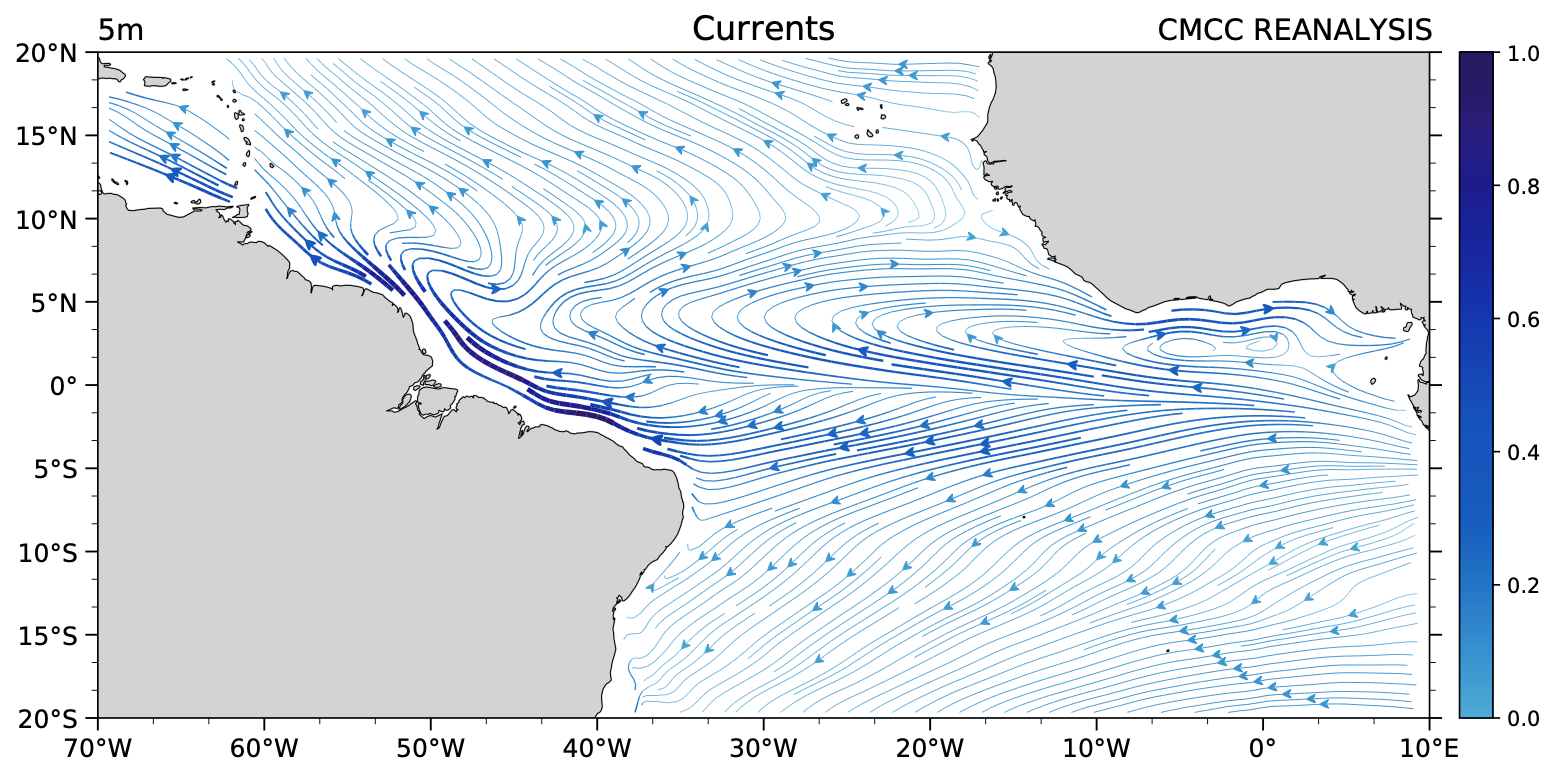
\includegraphics[width = .7 \textwidth]{figs/GD/UVstream5mATLEQ.png}
\caption{} \label{fig:}
\end{figure}

\subsubsection{The Gulf Stream}\label{the-gulf-stream}

The current system of the Gulf Stream is one of the major feature of the
global ocean circulation. It is shown in Fig.

\begin{figure}
\centering
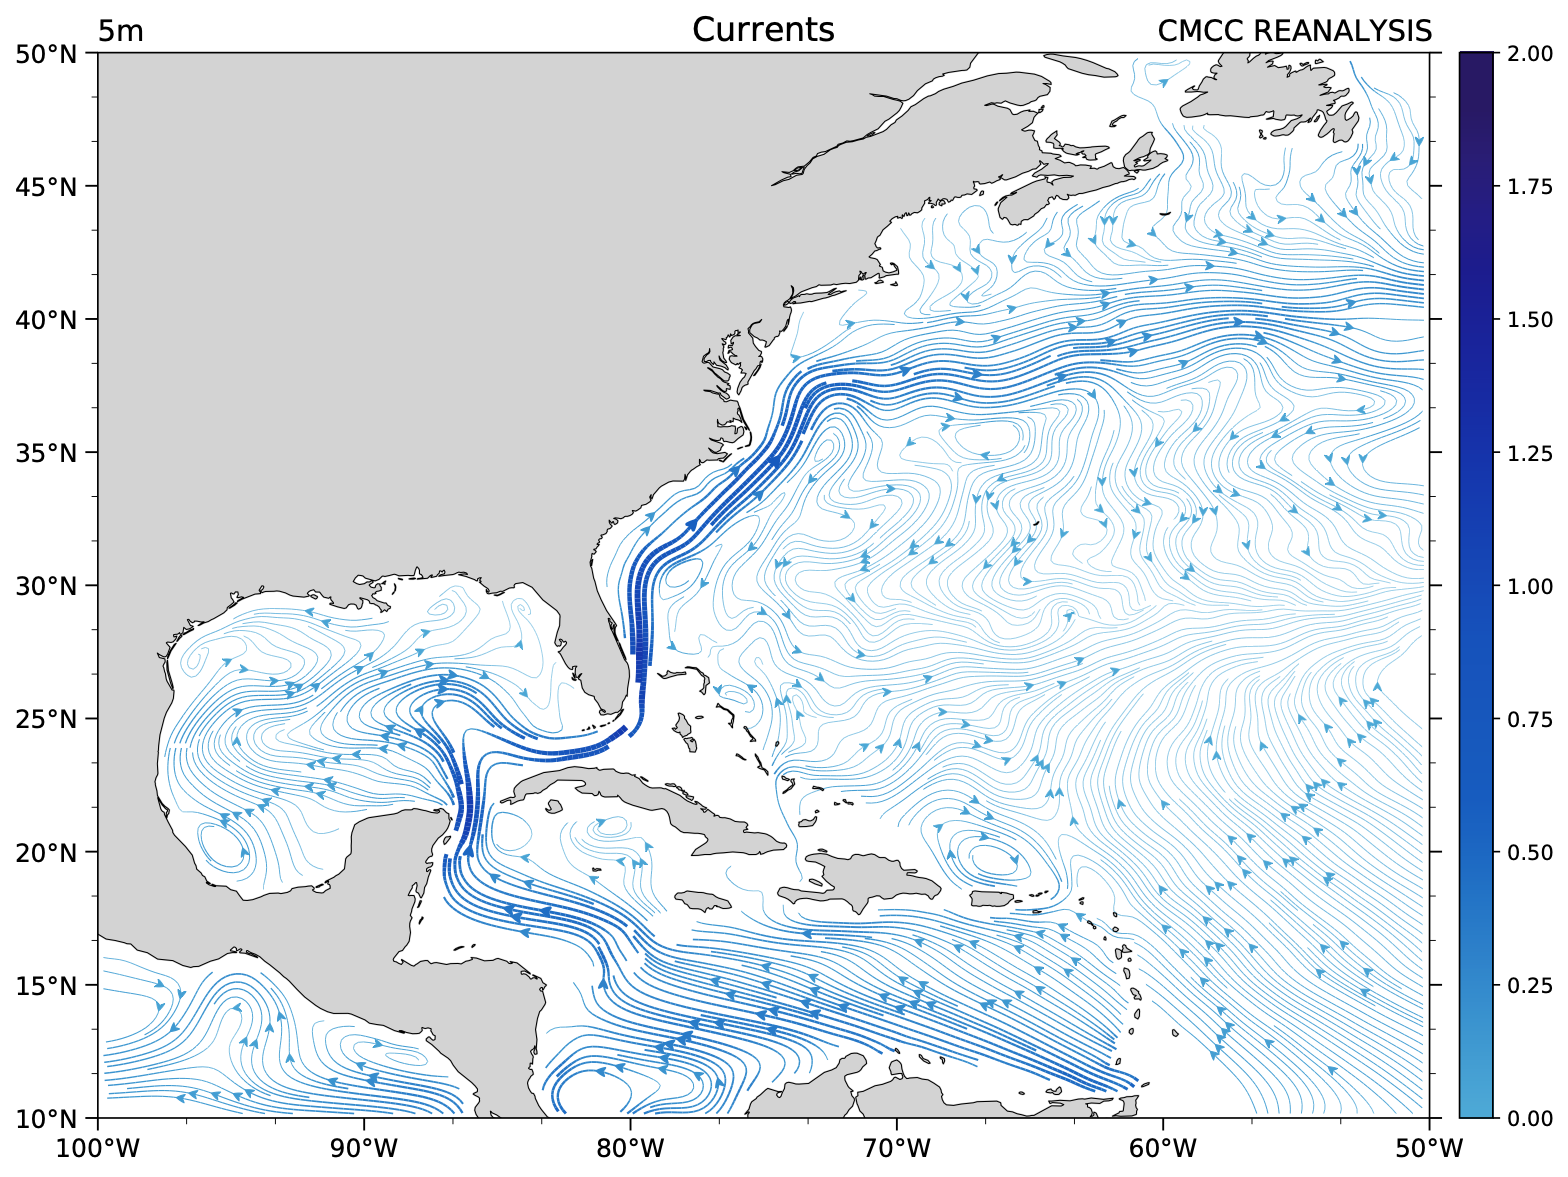
\includegraphics[width = .7 \textwidth]{figs/GD/UVstream5mATLCARIB.png}
\caption{} \label{fig:}
\end{figure}

\begin{figure}
\centering
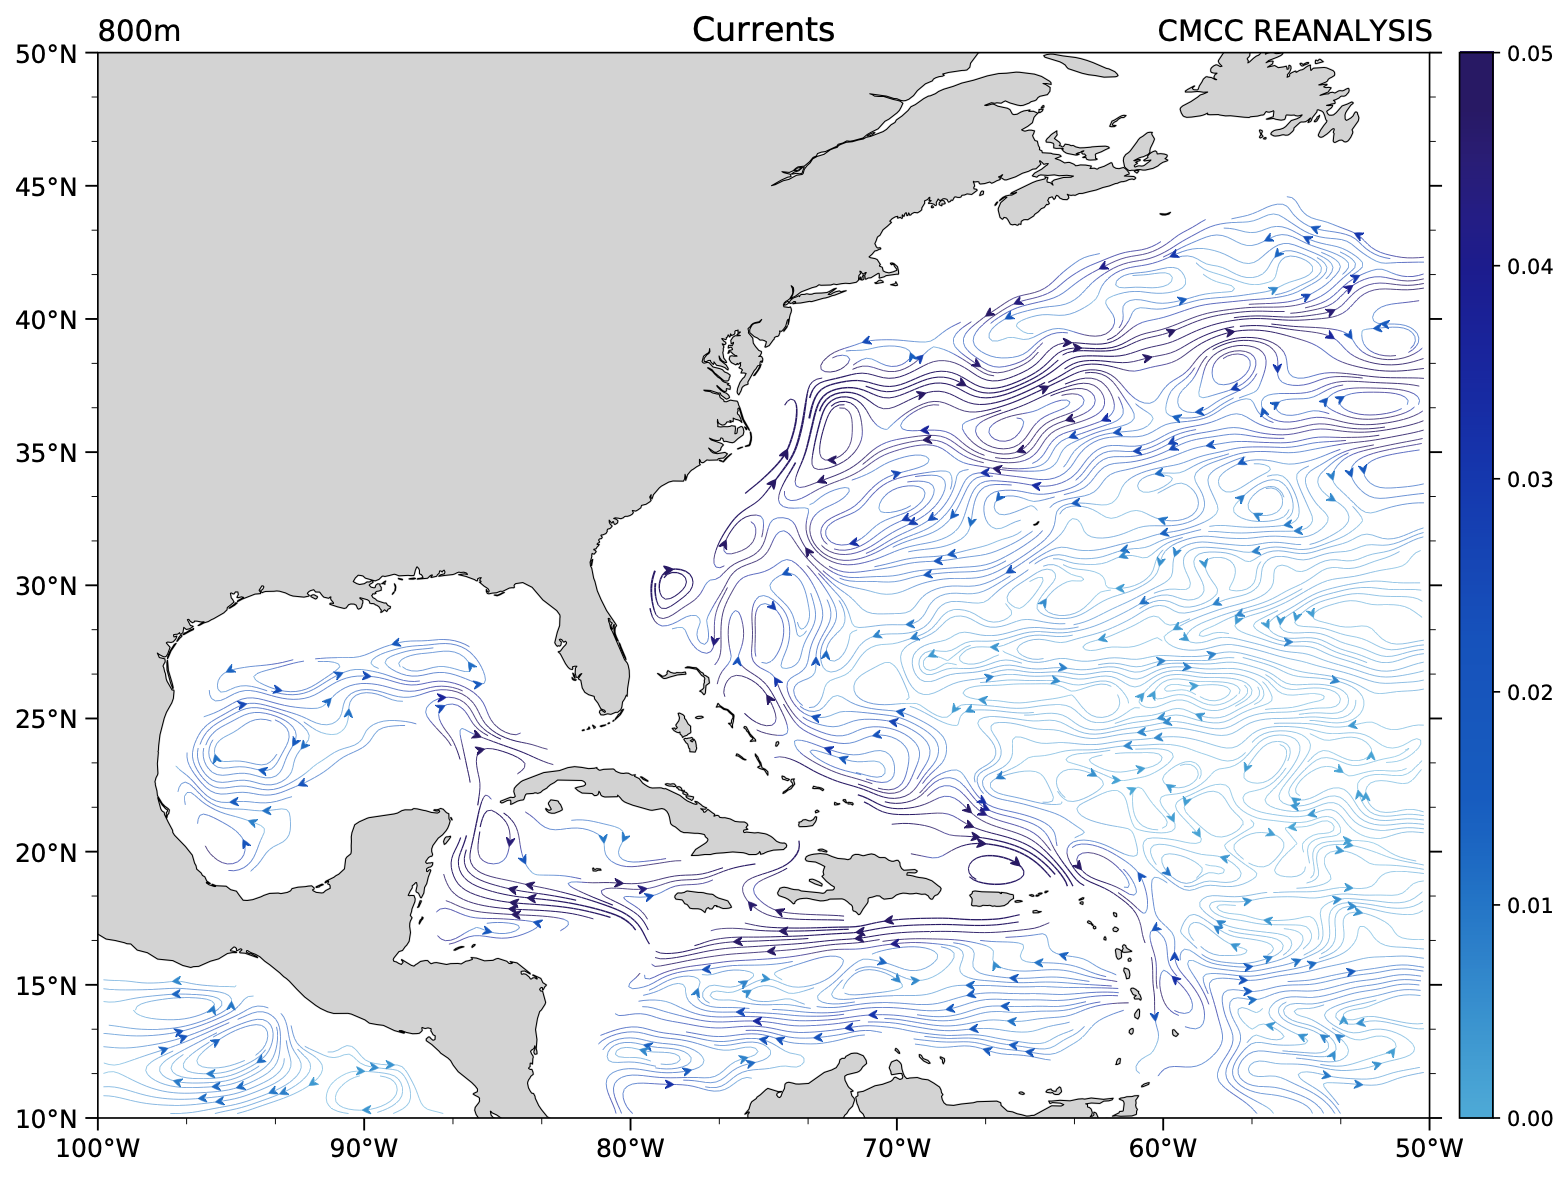
\includegraphics[width = .7 \textwidth]{figs/GD/UVstream800mATLCARIB.png}
\caption{As in Fig. \texttt{fig:8110aa}, but at 800m depth.}
\end{figure}

\begin{figure}
\centering
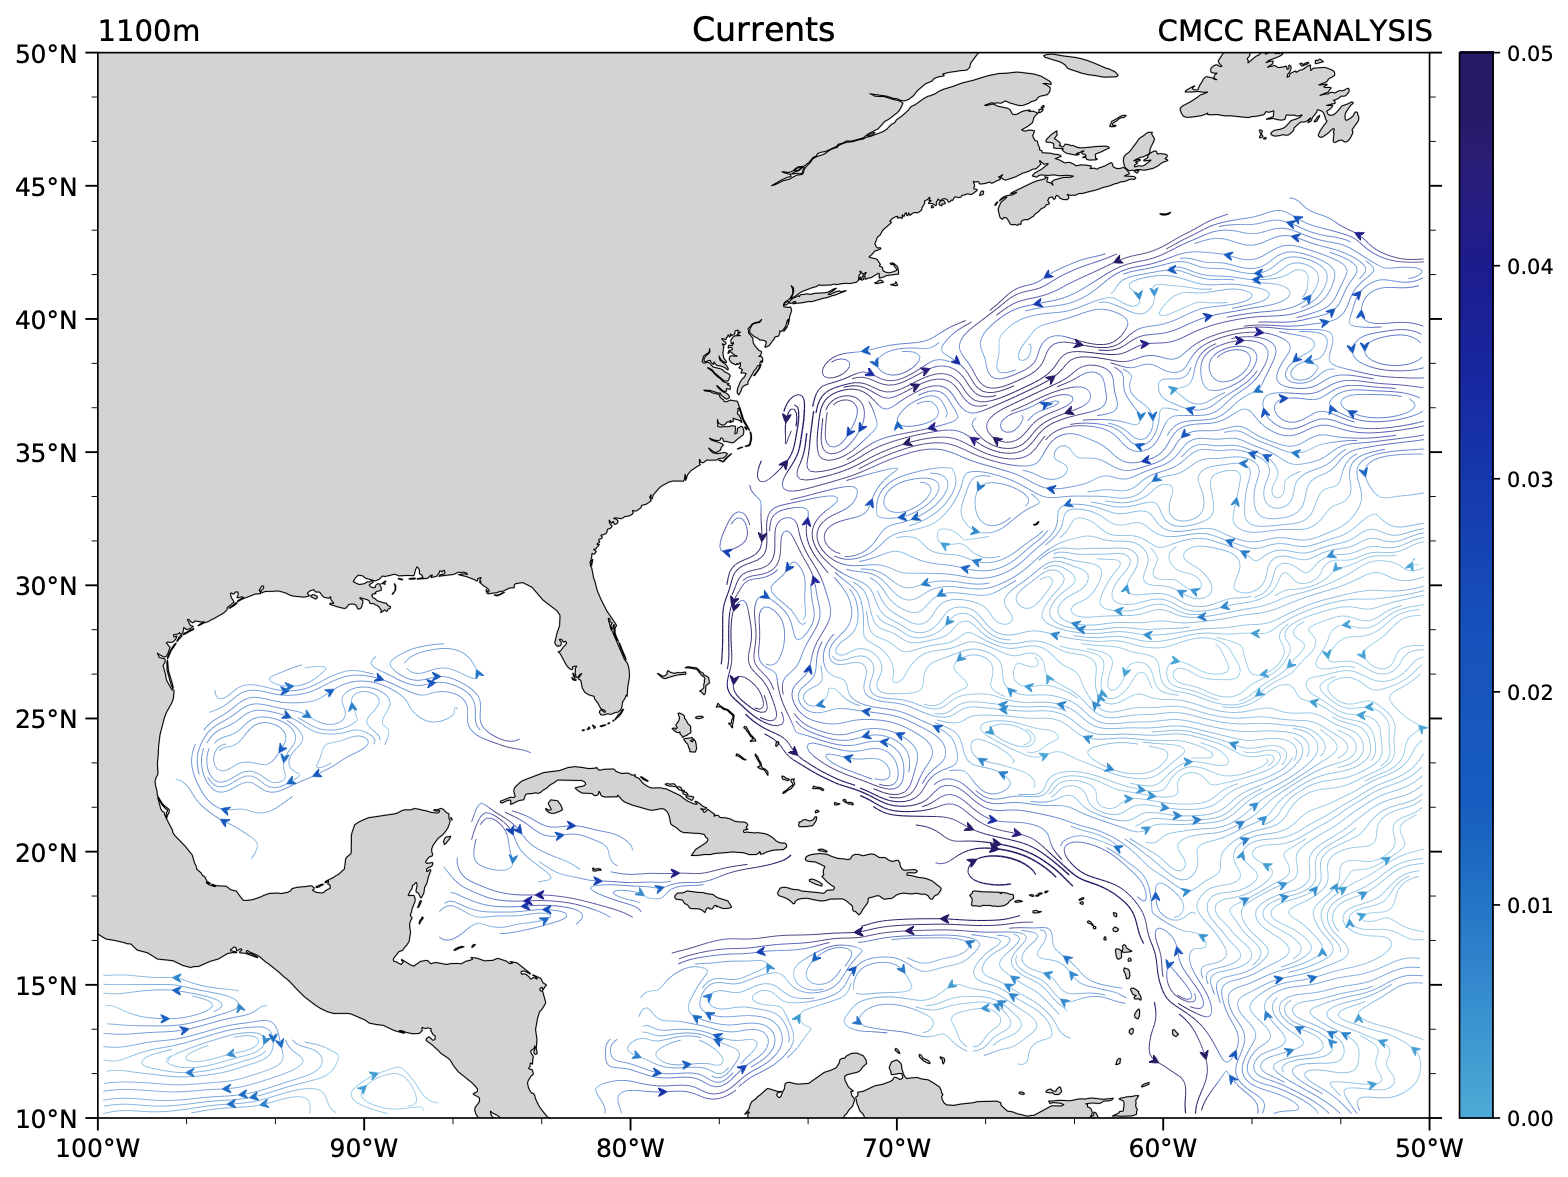
\includegraphics[width = .7 \textwidth]{figs/GD/UVstream1100mATLCARIB.png}
\caption{As in Fig. \texttt{fig:8110aa}, but at 1100m depth.}
\end{figure}

\begin{figure}
\centering
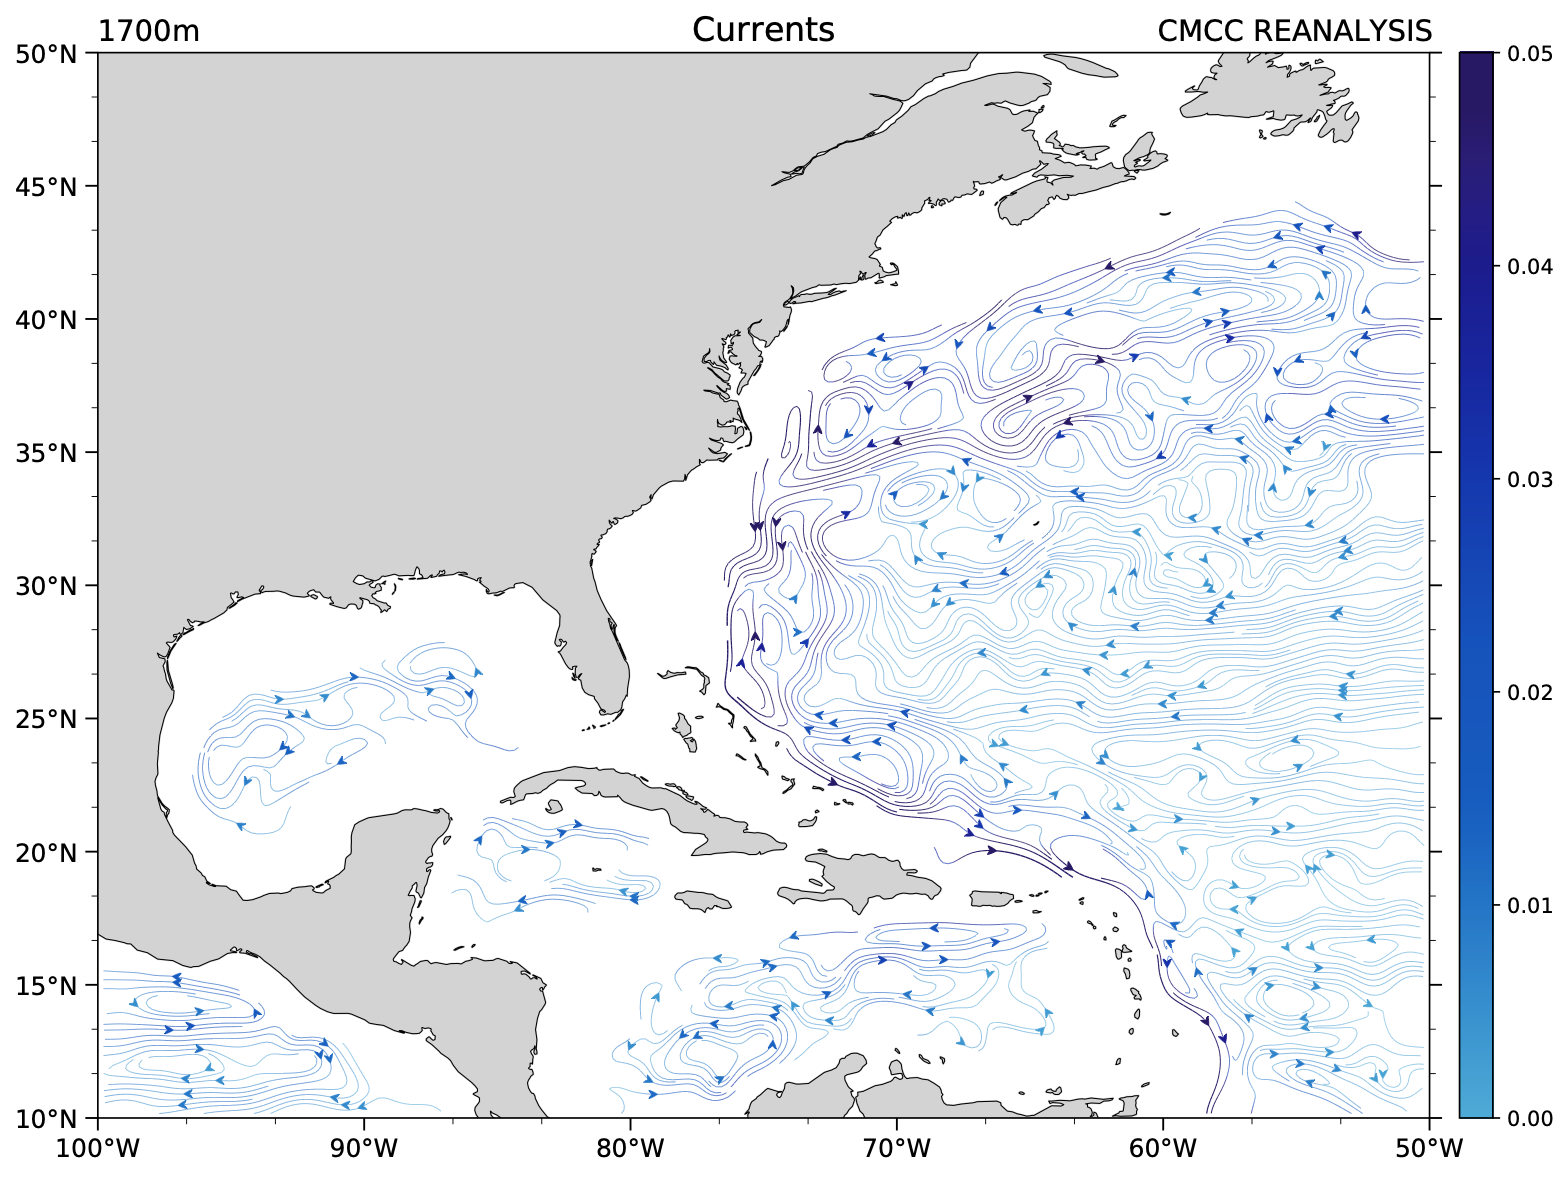
\includegraphics[width = .7 \textwidth]{figs/GD/UVstream1700mATLCARIB.png}
\caption{As in Fig. \texttt{fig:8110aa}, but at 1700m depth.}
\end{figure}

\subsubsection{The Kuroshio}\label{the-kuroshio}

The current system of the Kuroshio is one of the major feature of the
global ocean circulation. It is shown in Fig.

\begin{figure}
\centering
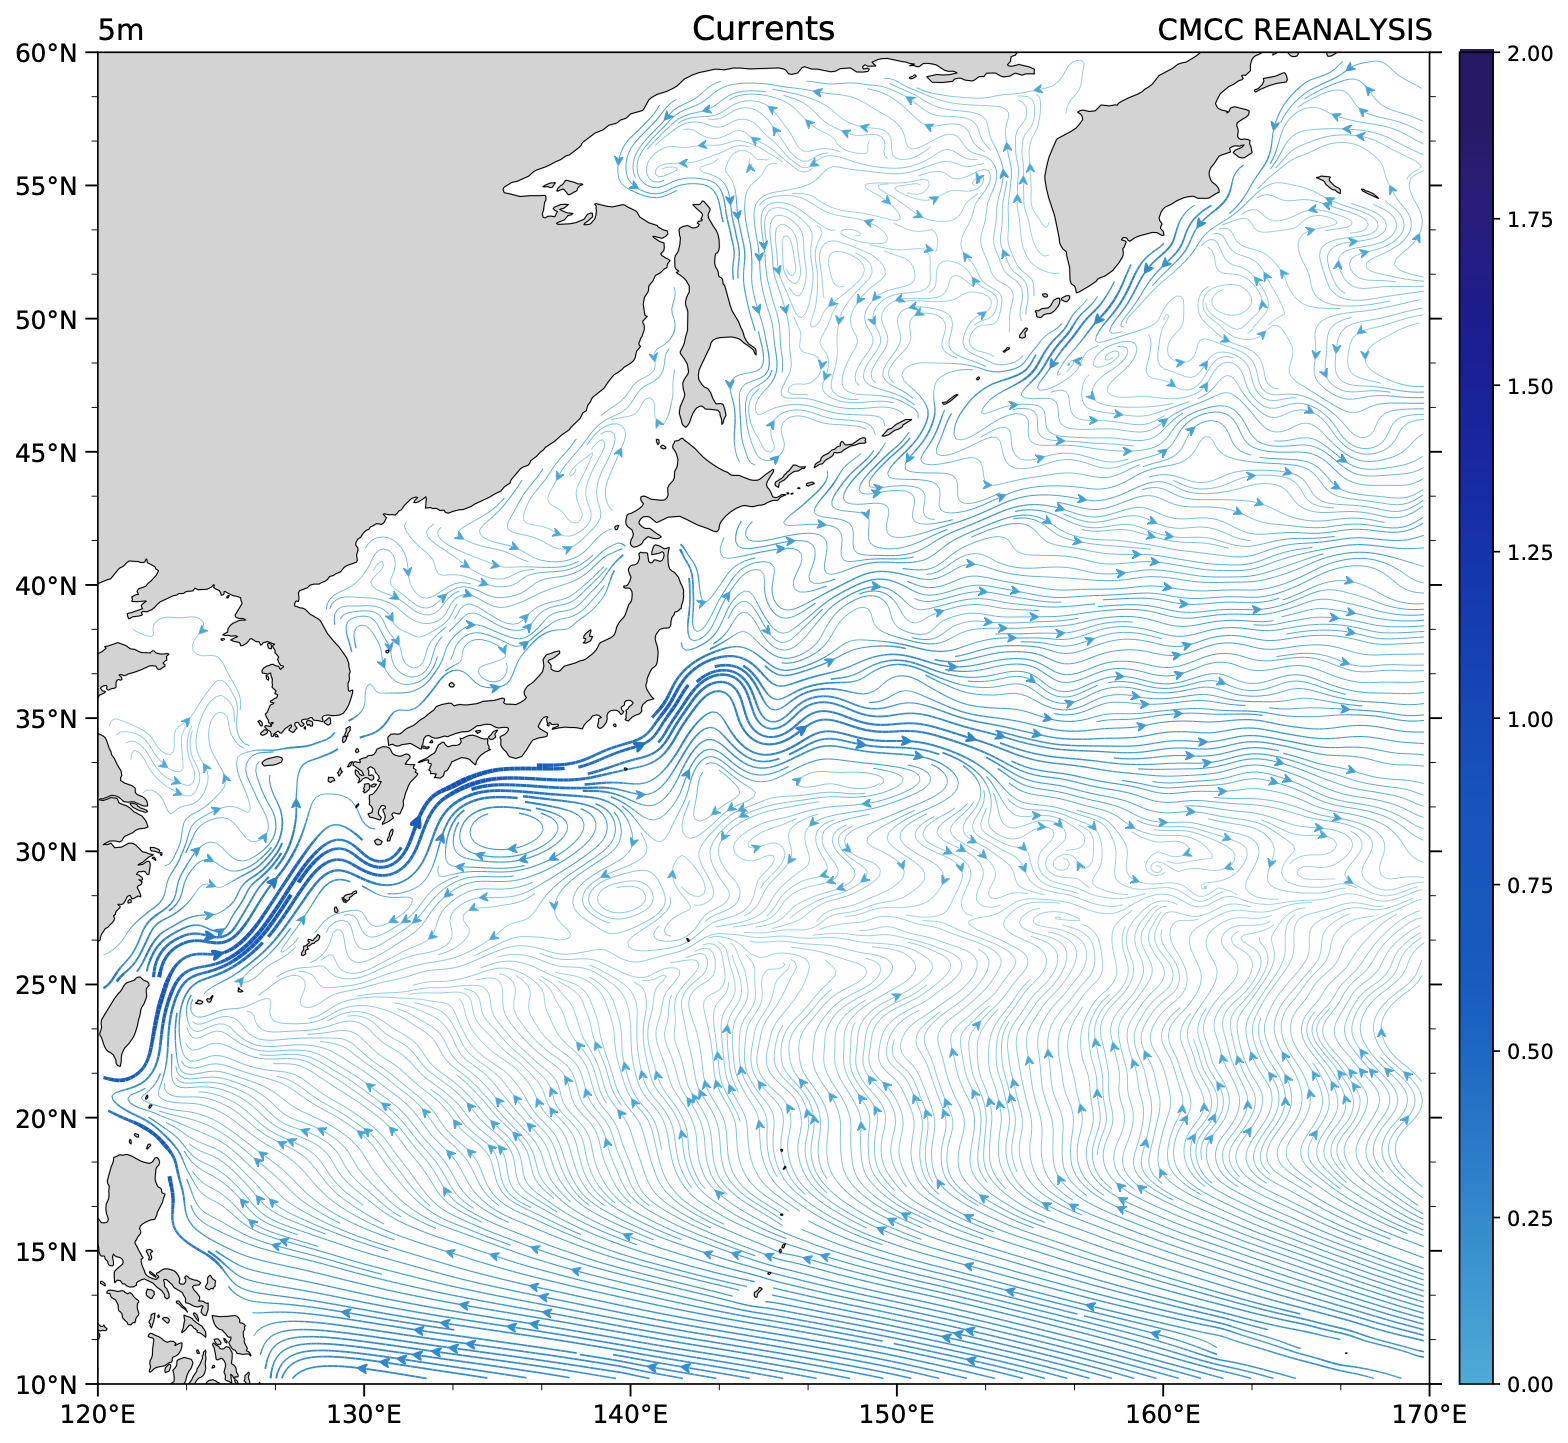
\includegraphics[width = .7 \textwidth]{figs/GD/UVstream5mKur.png}
\caption{} \label{fig:}
\end{figure}

\begin{figure}
\centering
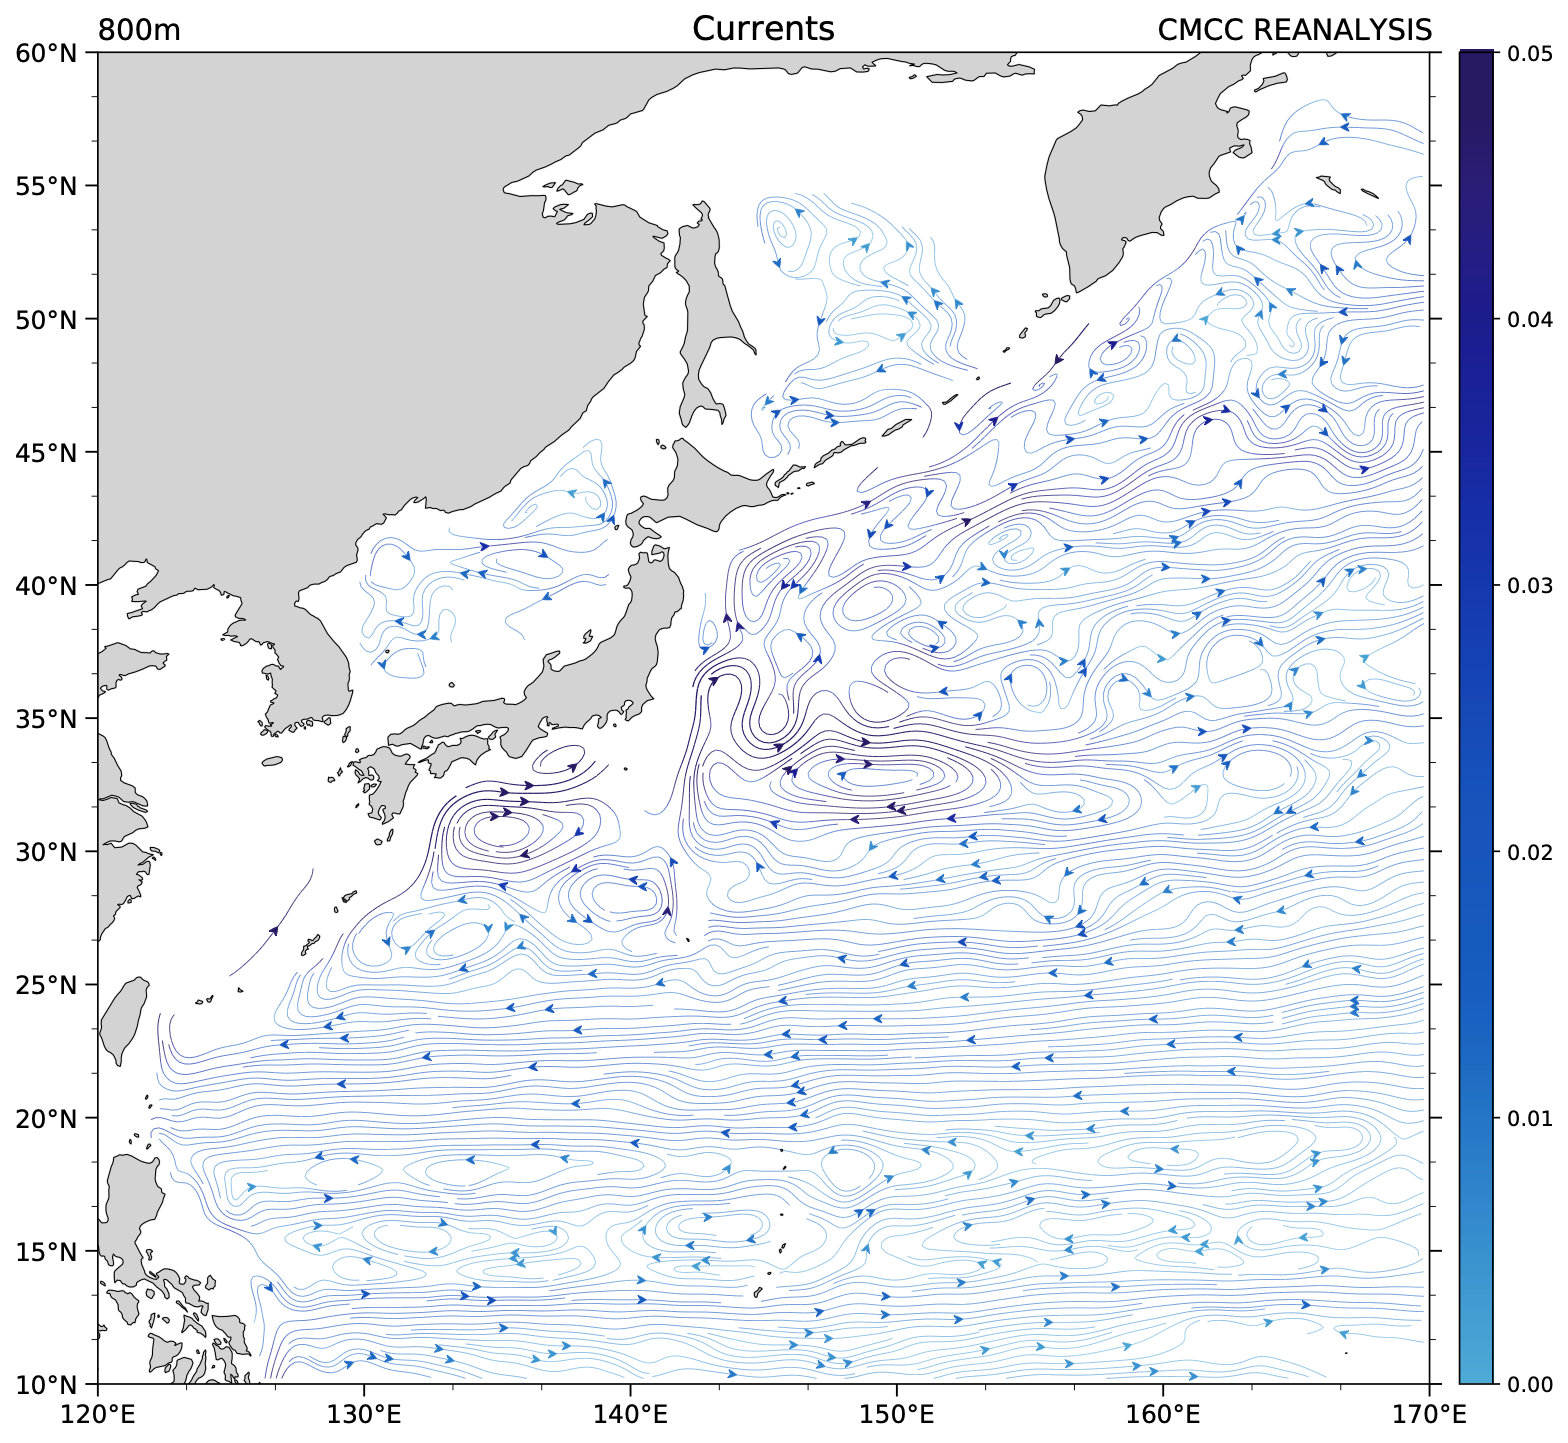
\includegraphics[width = .7 \textwidth]{figs/GD/UVstream800mKUR.png}
\caption{As in Fig. \texttt{fig:8111aa}, but at 800m depth.}
\end{figure}

\begin{figure}
\centering
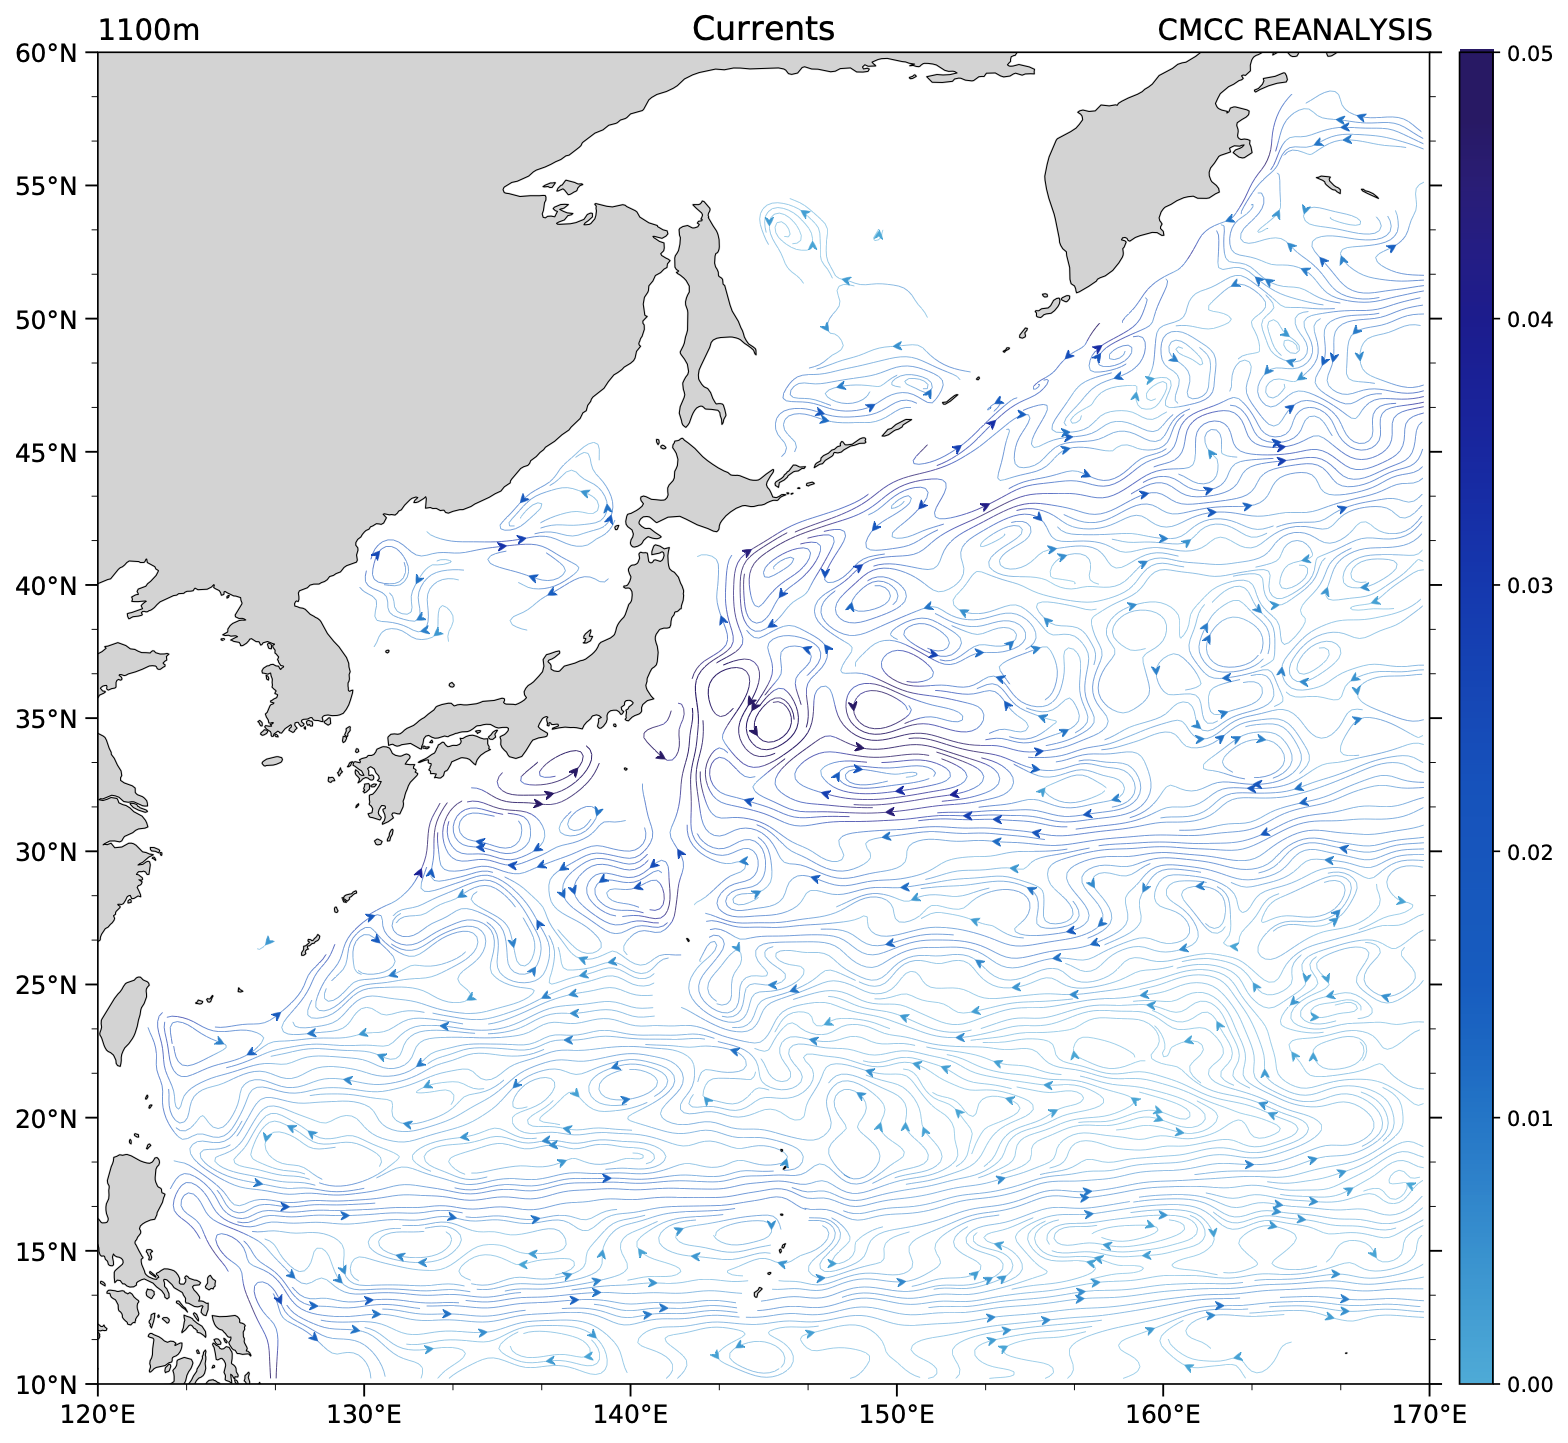
\includegraphics[width = .7 \textwidth]{figs/GD/UVstream1100mKUR.png}
\caption{As in Fig. \texttt{fig:8111aa}, but at 1100m depth.}
\end{figure}

\begin{figure}
\centering
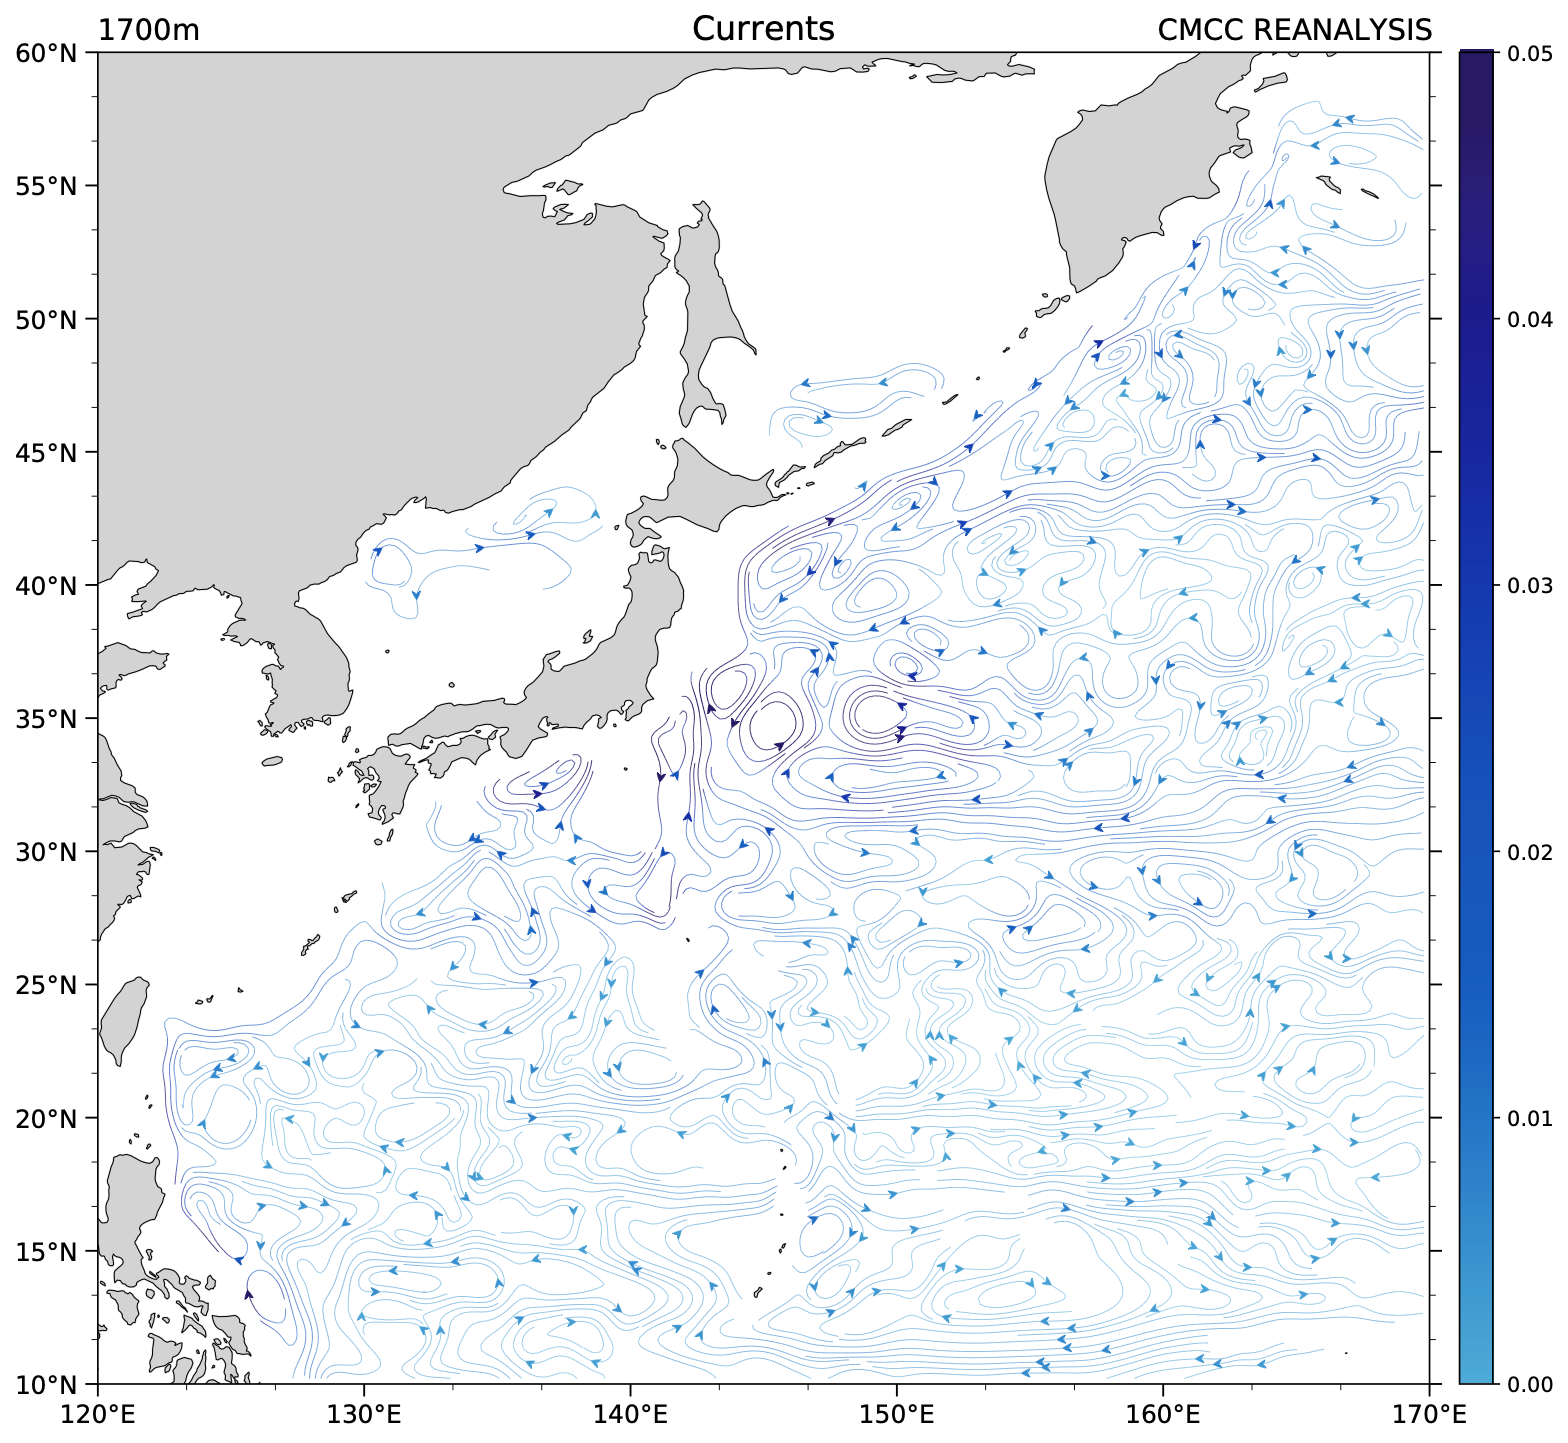
\includegraphics[width = .7 \textwidth]{figs/GD/UVstream1700mKUR.png}
\caption{As in Fig. \texttt{fig:8111aa}, but at 1700m depth.}
\end{figure}

\subsubsection{The upwelling zones}\label{the-upwelling-zones}

\begin{figure}
\centering
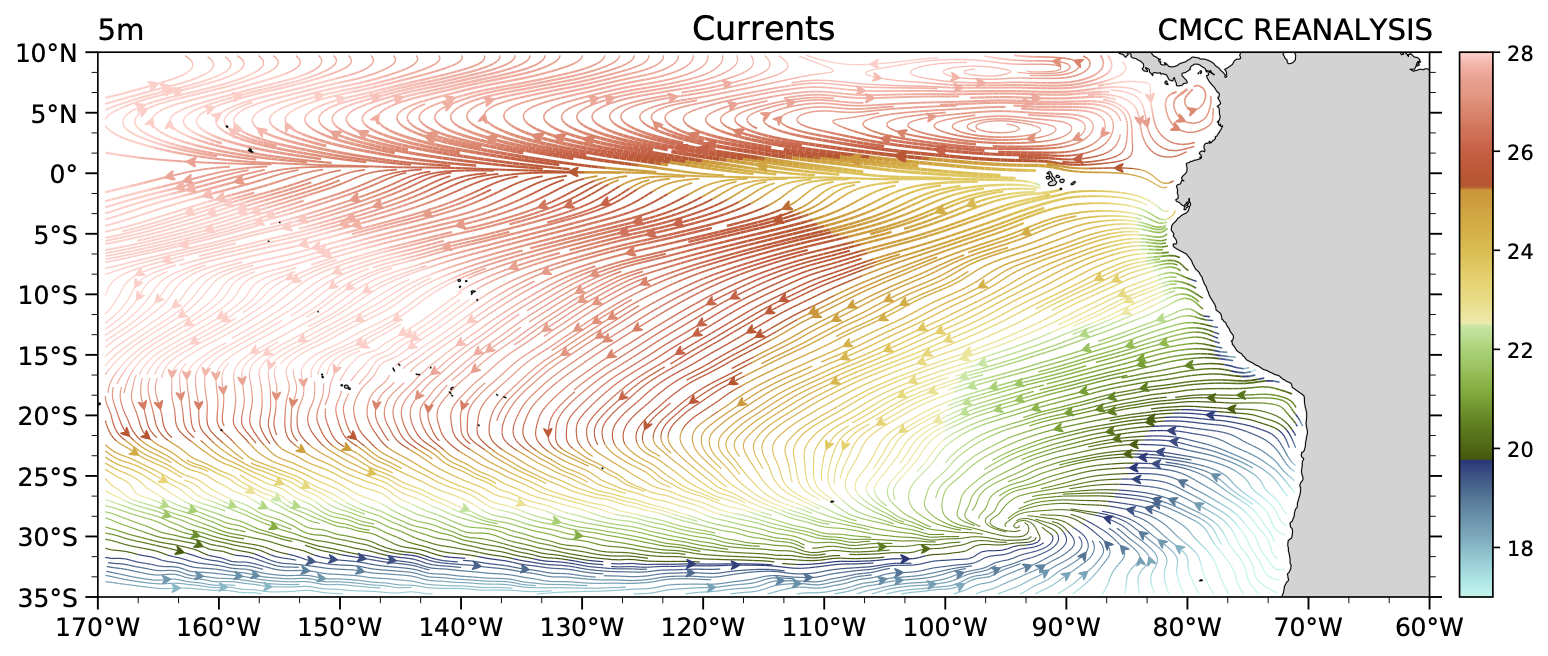
\includegraphics[width = .7 \textwidth]{figs/GD/UVstream5mSATemp.png}
\caption{} \label{fig:}
\end{figure}

\begin{figure}
\centering
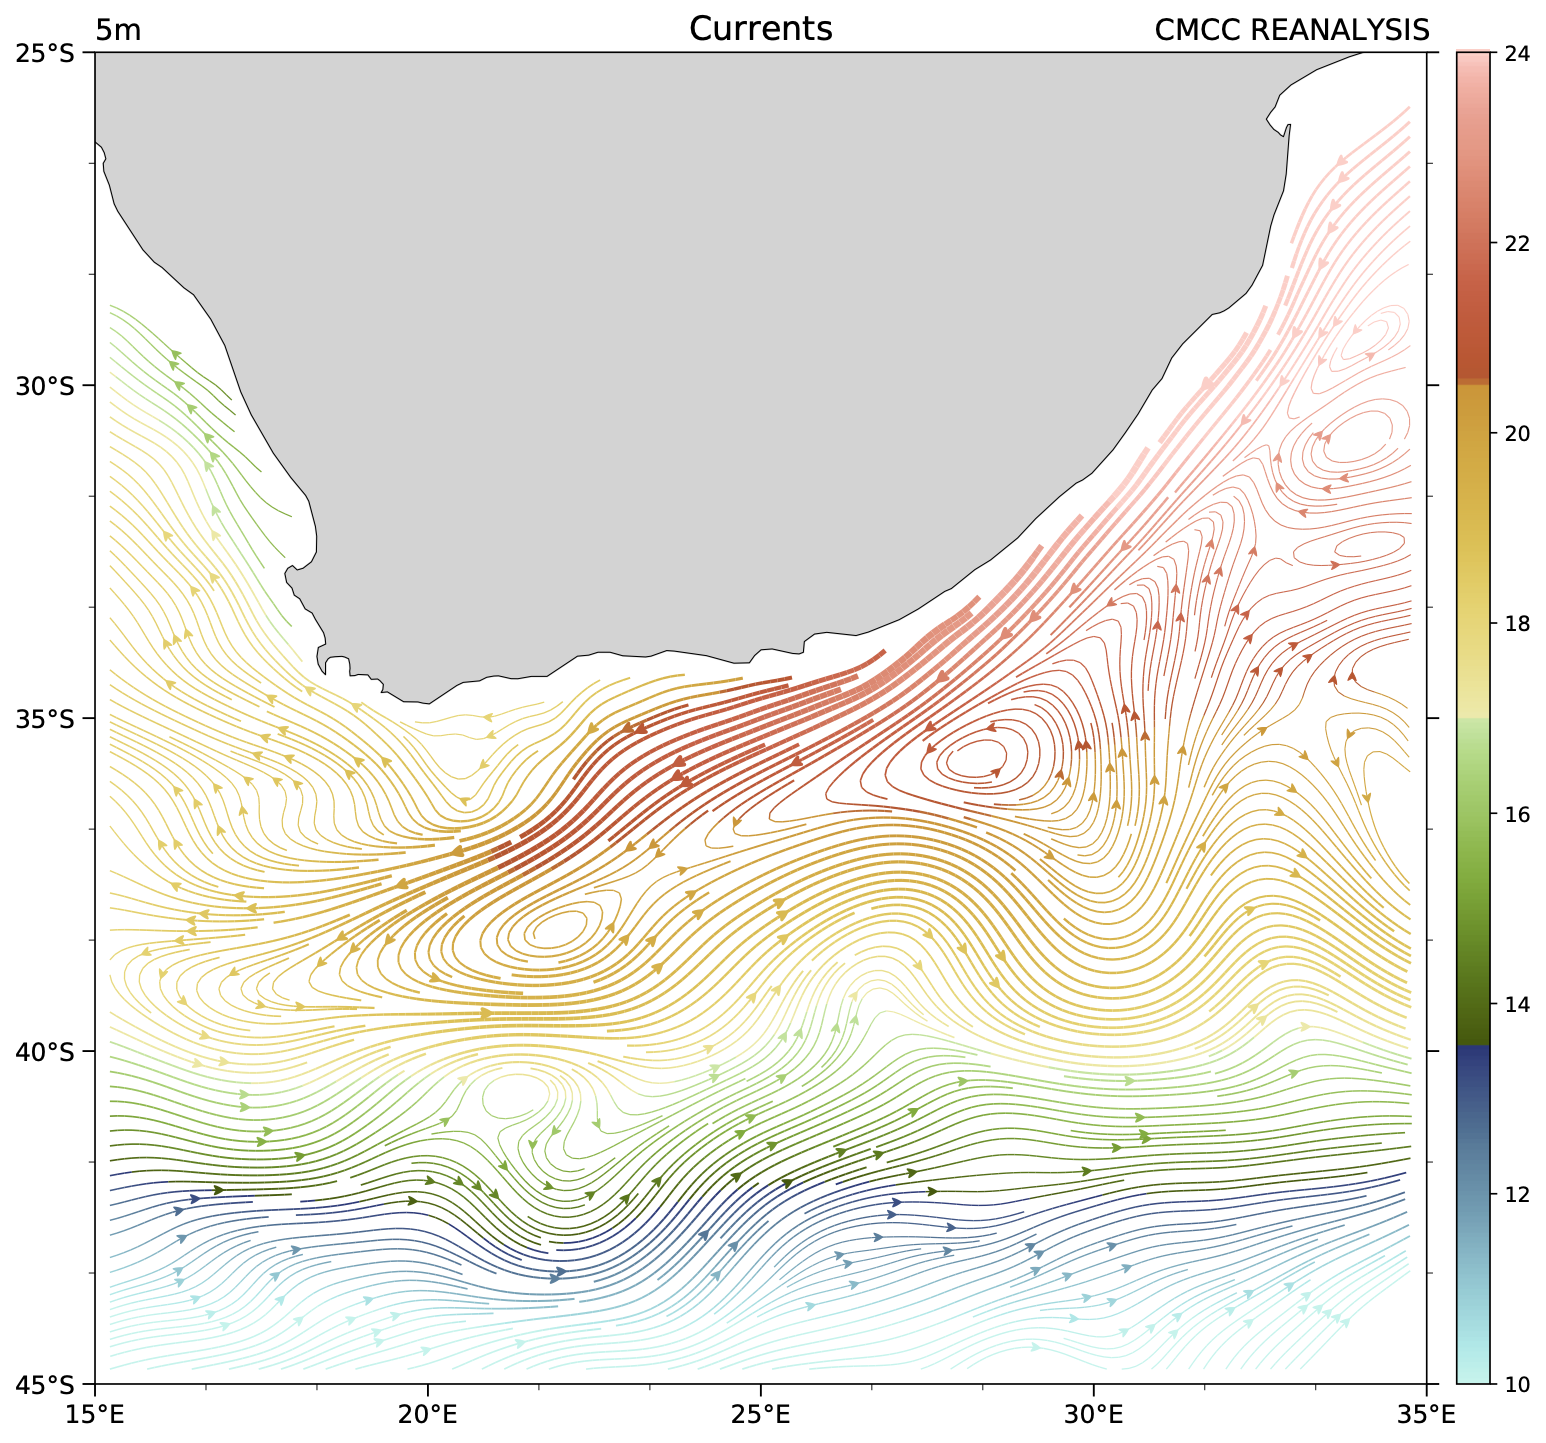
\includegraphics[width = .7 \textwidth]{figs/GD/UVstream5mAFRemp.png}
\caption{} \label{fig:}
\end{figure}

\subsubsection{The Somali Current}\label{the-somali-current}

\begin{figure}
\centering
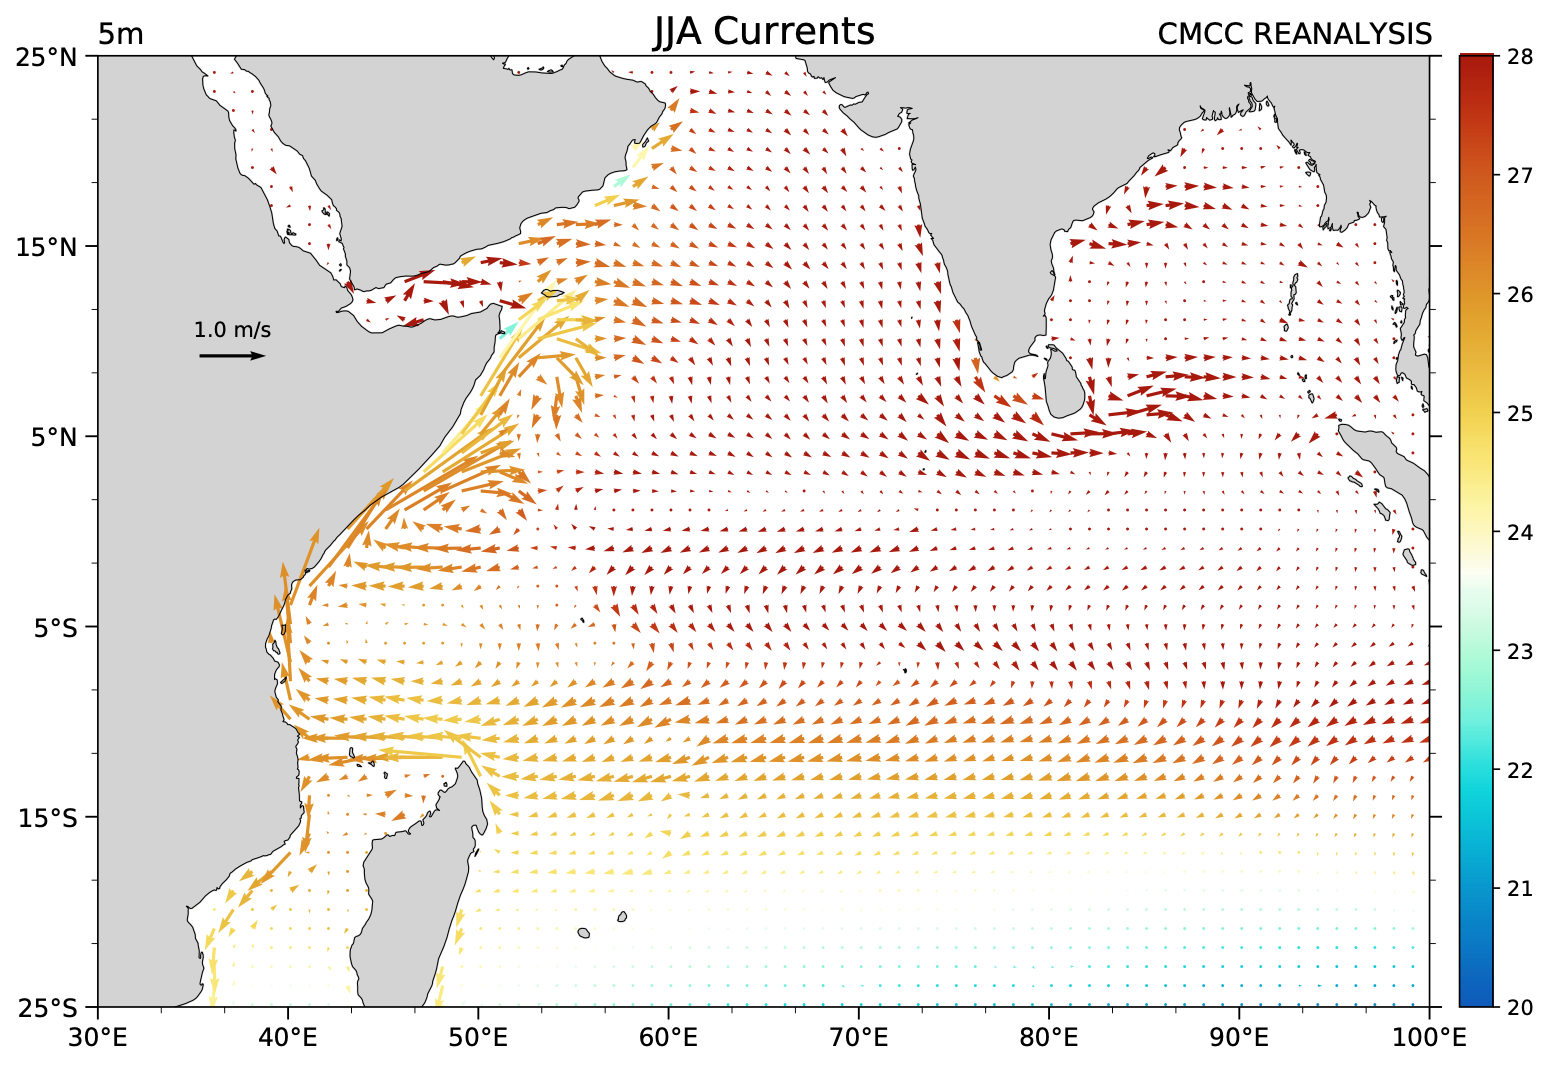
\includegraphics[width = .7 \textwidth]{figs/GD/UVvec5mSOMSUM.png}
\caption{} \label{fig:}
\end{figure}

\begin{figure}
\centering
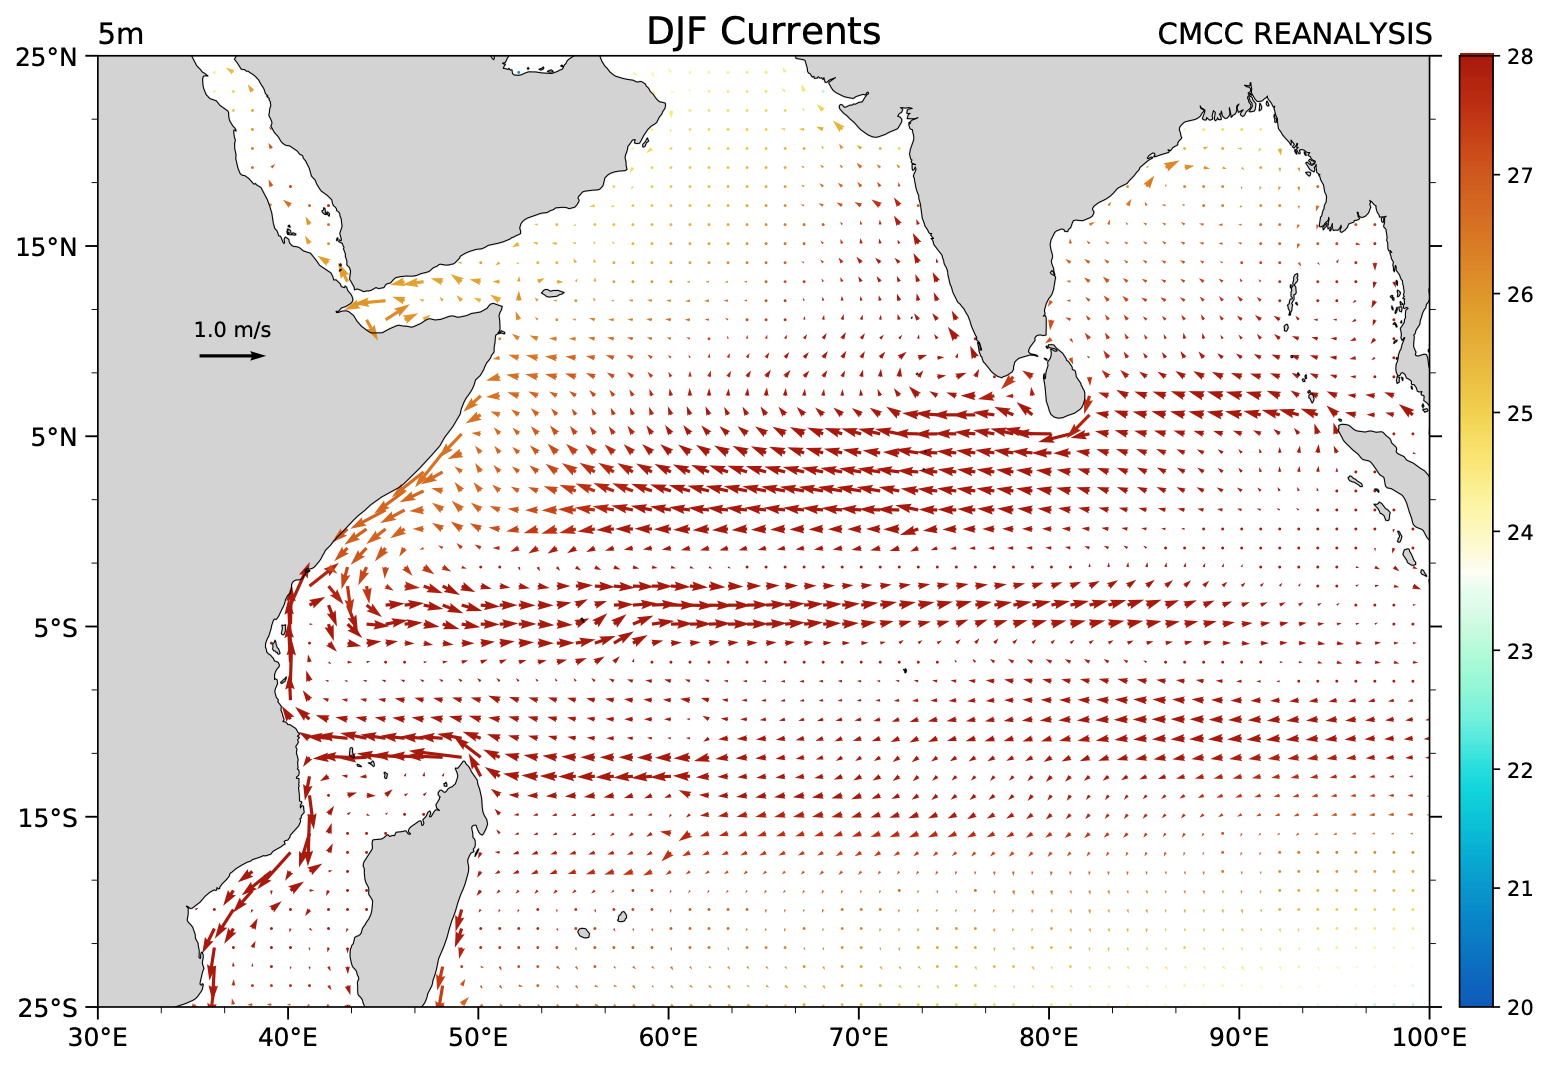
\includegraphics[width = .7 \textwidth]{figs/GD/UVvec5mSOMWIN.png}
\caption{As in Fig. \texttt{fig:8113a}, but for Summer.}
\end{figure}
